\chapter{Neuron Tissue Simulator (NTS)}
\label{chap:NTS}

NTS is a simulation system build upon the graph-based simulation system
(Sect.\ref{sec:graph-based-simulation}). A major part of the NTS is the
TissueFunctor (Sect.\ref{sec:TissueFunctor}).

\section{Introduction}


\subsection{Calculation variables}
\label{sec:calculation-variables}

Example of different {\bf calculation variables} (e.g. Voltage, $[\Ca]_i$,
NMDAR, $\Na$t (transient), $\Kdr$ channels, \ldots)

There are ??? types of calculation variables
\begin{enumerate}
  \item Compartment calculation variables (those with diffusion): Voltage,
  Calcium, CalciumER.

We needs to define : Branches, Junctions nodetypes. 

Junction nodetype is used to handle the branching junction, and the soma is
treated as a single junction with one or more dendrite trees.
  
  \item Channel calculation variables (Hodgkin-Huxley formulation,
  Markov-based models): Nat, Kdr, Nap, \ldots
  
  \item Synapses calculation variables: NMDAR (or if we want different models
  associated with different synapse's morphology: NMDARthin, NMDARmush), AMPAR.
  
  \item Presynaptic calculation variables:
\end{enumerate}

The different calculation variables are represented as different NodeTypes
(Sect.\ref{sec:NodeType-GSL}), each of them are mapped to a layers of different
category (e.g. Compartment, Channel, Synapse), and the layout functor will
distribute them to the right capsule, based on the criteria given in the proper
parameter file, e.g. CptParams.par (for Branching calculation variables),
ChanParams.par (for Channel calculation variables), SynParams.par (for (1)
defining what channels on what 'spine' neuron, (2) what Receptors on that spine)
etc.

Each capsule (Sect.\ref{sec:Capsule}) is uniquely identified using its
key of type \verb!SegmentDescriptor! (Sect.\ref{sec:SegmentDescriptor}).
% 
% The information above is part of the key associated with each segment (i.e. the
% \verb!_segmentDescriptor! data (Sect.\ref{sec:SegmentDescriptor}) for each
% Capsule - Sect.\ref{sec:Segment}). 
These parameter files have been passed to the TissueFunctor, so we just
reuse them by reusing the TissueFunctor functor to return a proper layout functor
(Sect.\ref{sec:functor-layout}).



\subsection{Branch concept: ComputeBranch}

A branch is stored in NTS as a ComputeBranch (Sect.\ref{sec:ComputeBranch})  not
necessarily a full branch from one branching-point to the next branching-point.

Based on Kozloski et al. (2011), a ComputeBranch is defined as a structure
spreading
\begin{itemize}
  \item from: the soma or from the junction point
  \item to: the end of the branch or to the capsule spanning across the slicing
  plane (Sect.\ref{sec:Decomposition})
\end{itemize}

{\it A ComputeBranch is an unbranched branch. In NEURON software, a similar
concept is {\bf section} - which is a continuous length of unbranched
cable; each section is ultimately discretized into compartments.}
(Sect.\ref{sec:compartment-in-neuron})

A neuron is organized into many ComputeBranch, each ComputeBranch is organized
into a number of capsules (Sect.\ref{sec:Capsule}), with capsules are ordered
from proximal to distal direction.
In NTS, we don't track Capsule, but we track Compartments
(Sect.\ref{sec:compartment-in-neuron}), which is a logical representation of a
number of capsules having the same value of Voltage, (or Calcium).

\subsection{Compartments concept (in NEURON - segment, in NTS - compartment)}
\label{sec:compartment-in-neuron}

\begin{mdframed}

In NEURON software,  each {\bf section} is represented by one or more {\bf
segments} of equal length. The number of segments is specified by the parameter
nseg, which can have a different value for each section. At the center of each
segment is a {\bf node}, the location where the internal voltage of the segment
is defined.

In NTS, each ComputeBranch is represented by one or more compartments of
potentially different lengths. NTS handles the processing non-uniform grid.
Similar to NEURON, the values of the quantitaties are defined at the node - the
center of the compartment.
\end{mdframed}

However, when solving the diffusion, they are treated at the level of
compartment, i.e. each branch has a list of compartments that are indexed from
distal to proximal end (following the Hines' ordering method).


The reason for using compartment is because we want to use a different indexing
scheme. Capsules are indexed from the soma (proximal to distal), while
\textcolor{red}{compartments are indexed from distal to proximal}, which is a
requirement for solving the tridiagonal matrix (Hines matrix) -
Sect.\ref{sec:Hines-matrix}.

Each compartment is a representation for one or many capsules
(Sect.\ref{sec:Capsule}).
\textcolor{red}{By default}, each compartment is the representation for only one
capsule which is represented as (x,y,z,r,dist2soma). We can change this by
supplying \verb!-r! option with the number of capsules per compartment (Sect.\ref{sec:TissueFunctor-how-to-create}). This
information is stored in \verb!_compartmentSize! data member of TissueFunctor
(Sect.\ref{sec:TissueFunctor-C++}). Also, at each branch, this information can
be retrieved through \verb!_nCapsules! data member of ComputeBranch class
(Sect.\ref{sec:ComputeBranch}).

When multiple capsules form a single compartment, the radius of the
two ends of the compartment is the average of the radius of the two ends of all
capsules
\begin{verbatim}
compartment.r = average(SUM(capsule.start.r))
compartment.end.r   = average(SUM(capsul.end.r))
\end{verbatim}

See DimensionStruct (Sect.\ref{sec:DimensionStruct}) introduced a representation
for a single compartment.

\begin{lstlisting}
//check TissueFunctor::compartmentalize(...)

     // compartment indexing is distal to proximal, while capsule
     // indexing is proximal to distal
 for (int i = 0, j = ncaps - ((ncaps % _compartmentSize == 0)
                                           ? _compartmentSize
                                           : ncaps % _compartmentSize);
               i < ncomps; ++i, j -= _compartmentSize)
{
  // i = index for compartment
  // j = index for capsules in the branch
  
     Capsule* begCap = &branch->_capsules[j];
     Capsule* endCap =
         &branch->_capsules[(i == 0) ? ncaps - 1
                       : j + _compartmentSize - 1];
     double radius = 0;
     // average all capsule radius to get the compartment's radius
     for (Capsule* capPtr = begCap; capPtr <= endCap; ++capPtr)
       radius += capPtr->getRadius();
     radius /= ((endCap - begCap) + 1);
	
	//the coord (x,y,z) of the compartment is 
	//         the average of the begin-coord of the firstcapsule 
	//                            end-coord of the last capsule
	//and return the Compartment data structure (x,y,z,r,dist2soma)
     StructDataItem* dimsDI = getDimension(
         lc, begCap->getBeginCoordinates(), endCap->getEndCoordinates(),
         radius, begCap->getDist2Soma());
     std::auto_ptr<DataItem> dimsDI_ap(dimsDI);
     NDPair* ndp = new NDPair("dimension", dimsDI_ap);

     NDPairList dimParams;
     dimParams.push_back(ndp);
     ct->getInstance(aptr_cst, dimParams, lc);
     ConstantDataItem* cdi =
         dynamic_cast<ConstantDataItem*>(aptr_cst.get());
     std::auto_ptr<Constant> aptr_dim;
     cdi->getConstant()->duplicate(aptr_dim);
     Constant* dim = aptr_dim.release();
     dimensions.push_back(dynamic_cast<CG_CompartmentDimension*>(dim));
}


ComputeBranch* branch = 0;
  //nodeIndex = (*node)->getNodeIndex();
  //nodeType = nodekind[1], i.e. the name passed to nodekind in LAYER
  //          statement, e.g  "Voltage", "Calcium" 
  // densityIndex = (*node)->getDensityIndex();
  
  branch = findBranch(nodeIndex, densityIndex, nodeType);

  int ncaps = branch->_nCapsules;
\end{lstlisting}



\subsection{Junction concept}
\label{sec:junction-in-NTS}

\begin{mdframed}

In NEURON software, the spherical soma is represented by a cylinder with the
same surface area as the sphere.
\end{mdframed}




\subsection{Compute Order: Compartment, EndPoint, Junction, JunctionPoint}

The original Hines' matrix allows solving the diffusion along every compartment
sequentially, i.e. a single linear system for the entire neuron (using implicit
numerical scheme).

Rempe-Chopp method introduces an explicit predictor-corrector scheme at branch
point (or junction point, i.e. the point where the branching occur), i.e. 
\verb!MAX_COMPUTE_ORDER=0!.

Kozloski et al. combine the two methods by combinding both of them with 
a user-defined value for \verb!MAX_COMPUTE_ORDER! (in the range implemented is
0 to 7). So, if \verb!MAX_COMPUTE_ORDER = 2!

A computeOrder for any tree is always start from zero. So, if a tree is cut by
the neuronpartitioner and put into 2 different MPI process, then computeOrder
for the first branch on the second half of the tree is restarted from zero,
regardless of the computeOrder of the last branch of the first half of the tree.


\section{New functors}

Unlike NEURONS (Sect.\ref{sec:NEURON}) and other approaches, 
the neurons are divided at points within branches
\begin{itemize}
  \item a single branch with a given number of compartments
  can be divided into 2 branches when it intersects with a slicing plane
  (which divides the tissue into different regions to be handled by different
  MPI processes). The method to divide is handled by a class called
  Decomposition or its derivatives - Sect.\ref{sec:Decomposition}.
  
NOTE: The slicing ensures the weighted histogram at all MPI processes are
uniform. Weight for each volume is the sum of all weights of compartments in
that volume. Weights for each compartment are calculated based on a sum of
weights of its associated channel and branch models.

If a slicing plane cut through a compartment, that compartment is then assigned
to the volume containing the compartment's proximal endpoint.
  
  \item branches whose compartments were assigned to more than one volume are
  effectively cut into multiple branches.
  
The communication between 2 compartments on two different MPI processes are done
through the proxies nodes.
\end{itemize}

Physiological initialization requires iterating through branch segments and
touches, and identifying which segments require connections to local
instantiations of the neural tissue models, and which must connect to model
proxies. Multiple searches of multiple maps that
relate the various models to each other, and to the tissue volume
decomposition via \verb!std::map! container in C++ language.

\begin{enumerate}
  \item NEURON: A single linear system at which all compartments are solved
  sequentially (i.e. Gaussian forward elimination) based upon a given indexing
  scheme.  \textcolor{red}{The fully implicit method of Hines' matrix provides
  unconditional stability, but it is slow.}
  
  Here, the junction is not treated as a compartment.
\begin{verbatim}
// NOTE: There is no junction
// compartments in all branches of a neuron are indexed sequentially
Gaussian forward elimination for each compartment 
  
\end{verbatim}  
  
  \item Rempe-Chopp: Each branch are solved independently, with junction is
  organized as an explicit predictor-corrector.
   \textcolor{red}{The implicit/explicit numerical method by Rempe-Chopp
   provides parallelism}.
  
 Here, the junction is treated as a compartment. 
   
\begin{verbatim}
parallelfor branch do  //time-step = dt/2 
   Gausian-forward-solve compartments on that branch sequentially
   
predict-of-Vm-at-all-explicit-junctions

parallelfor branch do //time-step = dt/2
   Gausian-backward-solve compartments on that branch sequentially

correct-of-Vm-at-all-explicit-junctions   
\end{verbatim}
Gaussian-forward-solve = forward-elimination starting from compartment 0 to end.
Gaussian-backward-solve = forward-elimination starting from compartment end to
0.

   \item Kozloski et al: fully-implicit approach like Hine's method but 
   treat the junction as a compartment, i.e. implicit junction.

\begin{verbatim}
// NOTE: every junction is treated as a compartment (i.e. implicit
//       junction)
// compartments in all branches of a neuron are indexed sequentially
Gaussian forward elimination for each compartment 
  
\end{verbatim}  
   
   
   \item Kozloski et al: introduced the concept of computeOrder, which is defined as the
   number of junctions from the branch and the soma;
   and \verb!MAX_COMPUTE_ORDER!, as the limit for resting the computeOrder.
    \textcolor{red}{The hybrid method combines the trade-off of
    the accuracy and stability between the two methods}.
      
 \begin{verbatim}
// NOTE: every junction is treated as a compartment 
//  (i.e. a junction is implicit junction (if computeOrder of the previous
//                         branch is smaller than MAX_COMPUTE_ORDER
//    or             is explicit junction (if computeOrder of the previous
//                         branch is MAX_COMPUTE_ORDER
//  )
// compartments in all branches of a neuron are indexed sequentially

for computeOrder = 0 to MAX_COMPUTE_ORDER do
   parallelfor branch of given computeOrder do  //time-step = dt/2 
      Gausian-forward-solve compartments on that branch sequentially
   
predict-of-Vm-at-all-explicit-junctions

for computeOrder = 0 to MAX_COMPUTE_ORDER do
   parallelfor branch of given computeOrder do //time-step = dt/2
      Gausian-backward-solve compartments on that branch sequentially

correct-of-Vm-at-all-explicit-junctions   
\end{verbatim}
      
   
   Branches are assigned with a computeOrder, starting with 0 for branches
   stemming out from soma, and increase at each junction, There are two
   scenarios for resetting the computeOrder, before increasing again
   \begin{itemize}
     \item the computeorder reaches \verb!MAX_COMPUTE_ORDER!.
     
     \item the branch is cut by the slicing plane.
     
     To achieve a volume decomposition, additional junctions (either implicit or
     explicit) may be added at cut points between volumes, thereby altering all
     distal compute orders, and changing the numerical approach
     (explicit/implicit) for solving certain distal junctions.
     
%     Then and  end-point is put to indicating ending a branch at that     
   \end{itemize}
    
    Here, the junction is treated as a single-compartment branch which can be 
    \begin{itemize}
      \item implicit junction: it is part of the linear system
      
      \item explicit junction: face the branch with computeOrder
      \verb!MAX_COMPUTE_ORDER-1!.
    \end{itemize}
Hines' approach is replicated with all junctions being implicit.

% \begin{verbatim}
% for computeOrder = 0 to MAX_COMPUTE_ORDER do
%    parallelfor branch of given computeOrder do  //time-step = dt/2 
%       Gausian-forward-solve compartments on that branch sequentially
%    
% predict-of-Vm-at-all-explicit-junctions
% 
% for computeOrder = 0 to MAX_COMPUTE_ORDER do
%    parallelfor branch of given computeOrder do //time-step = dt/2
%       Gausian-backward-solve compartments on that branch sequentially
% 
% correct-of-Vm-at-all-explicit-junctions   
% \end{verbatim}
%     
   NOTE: Branches of the same computeOrder are computed in parallel.
So, Rempe-Chopp is a special case of Kozloski et al.'s method when
\verb!MAX_COMPUTE_ORDER! is larger than the maximum number of branching in all
neurons.
    
\end{enumerate}


\subsection{TissueFunctor}
\label{sec:TissueFunctor.mdl}

TissueFunctor is a functor of category 'FUNCTOR'. Like any other functor
(Sect.\ref{sec:Functor-in-MDL}), we need to define (1) interface for functor
creation, (2) interface for functor's kernel that is invoked each time the
functor is called:
in the *.gsl script.

//MDL script
\begin{verbatim}
Framework Functor TissueFunctor Category "FUNCTOR" {
   Initialize(string commandLineArgs1, 
              string commandLineArgs2, string compartmentParamFile, 
              string channelParamFile, 
              string synapseParamFile, 
              Functor* layoutFunctor, 
              Functor*
      nodeInitFunctor, 
              Functor* connectorFunctor, 
              Functor* probeFunctor); 
              
  Functor* Execute(string tissueElement, NDPairList* params); }
\end{verbatim}

In the GSL script, we need to define this functor.
This functor, once being called, depending on the context (of where it
is called in the GSL script), it will returns a new proper functor (either
TissueLayoutFunctor, TissueConnectorFunctor or TissueNodeInitFunctor). 
Importantly, each of the newly created functor has a data member to reference
back to the original TissueFunctor instance.



% MDL: 
% \begin{verbatim}
% #ifndef TissueFunctor_MDL                                                                                     
% #define TissueFunctor_MDL                                                                                     
%                                                                                                               
% Framework Functor TissueFunctor Category "FUNCTOR" {                                                                                                                                                   
%    Initialize(string commandLineArgs1, string commandLineArgs2, 
%               string compartmentParamFile, string channelParamFile, 
%               string synapseParamFile, 
%               Functor* layoutFunctor, 
%               Functor* nodeInitFunctor, 
%               Functor* connectorFunctor, 
%               Functor* probeFunctor); 
%               
%    Functor* Execute(string tissueElement, NDPairList* params);                                                    
% }                                                                                                             
%                                                                                                               
% #endif  
% \end{verbatim}

\textcolor{red}{\bf IMPORTANT:} Here, the functor is designed to perform
different roles, depending upon the content of \verb!tissueElement! string 
\begin{enumerate}
  \item as a Layout functor - Sect.\ref{sec:TissueFunctor-as-layout-functor}
  \item as a Probe functor - Sect.\ref{sec:TissueFunctor-as-probe-functor}
  \item as a NodeInit functor - Sect.\ref{sec:TissueFunctor-as-nodeinit-functor}
  \item as a Connect functor -
  Sect.\ref{sec:TissueFunctor-as-connector-functor}
\end{enumerate}

\subsection{- get access to data passed to the functors}
\label{sec:TissueFunctor-get-access-to-passed-data}

Each time we call the TissueFunctor functor, the \verb!userExecute()! is evoked
in which the last argument is the data passed to it as NDPairList
(Sect.\ref{sec:NDPairList}) and the first argument is a string being used as an
indicator how the TissueFunctor's behavior should be
\begin{verbatim}
std::auto_ptr<Functor> TissueFunctor::userExecute(LensContext* CG_c,
                                                  String& tissueElement,
                                                  NDPairList*& params) {

\end{verbatim}

\verb!tissueElement! as
\begin{itemize}
  \item ``Layout'' - Sect.\ref{sec:TissueFunctor-layout}
\begin{verbatim}
  if (tissueElement == "Layout")
  {
    TissueElement* element = dynamic_cast<TissueElement*>(_layoutFunctor.get());
    element->setTissueFunctor(this);
    _layoutFunctor->duplicate(rval);
  }
\end{verbatim}
  \item ``NodeInit'' - Sect.\ref{sec:TissueFunctor-NodeInit}
\begin{verbatim}
  else if (tissueElement == "NodeInit")
  {
    TissueElement* element =
        dynamic_cast<TissueElement*>(_nodeInitFunctor.get());
    element->setTissueFunctor(this);
    _nodeInitFunctor->duplicate(rval);
  }
\end{verbatim}
  \item ``Connect''  - Sect.\ref{sec:TissueFunctor-connect}
\begin{verbatim}
  else if (tissueElement == "Connect")
  {
    doConnector(CG_c);
  }
\end{verbatim}

which can be used as
\begin{verbatim}
// calling this is critical to establish 
// the connection between all kinds of node-type to
// the associated compartment variables (e.g. Voltage, Calcium)

tissueFunctor("Connect", <> ); 
\end{verbatim}
which calls
\begin{verbatim}
TissueFunctor::doConnector(CG_c);
\end{verbatim}



Basically, it does the same as ``Connector'' below.

  \item ``Connector'' - Sect.\ref{sec:TissueFunctor-as-connector-functor}
  
\begin{verbatim}
  else if (tissueElement == "Connector")
  {
    TissueElement* element =
        dynamic_cast<TissueElement*>(_connectorFunctor.get());
    element->setTissueFunctor(this);
    _connectorFunctor->duplicate(rval);
  }
\end{verbatim}
Basically, it does the same as ``Connect'' above.

  \item ``Probe'' - Sect.\ref{sec:TissueFunctor-probe}

\begin{verbatim}
  else if (tissueElement == "Probe")
  {
    TissueElement* element = dynamic_cast<TissueElement*>(_probeFunctor.get());
    element->setTissueFunctor(this);
    _probeFunctor->duplicate(rval);
  }
\end{verbatim}
\end{itemize}

Inside this method of TissueFunctor, we copy the parameters information the
private data member \verb!_params!
\begin{verbatim}
 params->duplicate(_params);
\end{verbatim}

\subsection{TissueLayoutFunctor: doLayout() as doLayoutNTS()}
\label{sec:TissueFunctor-layout}
\label{sec:TissueLayoutFunctor}


The class TissueLayoutFunctor also need to be derived from TissueElement class
(Sect.\ref{sec:TissueElement}). As a layout functor
(Sect.\ref{sec:functor-layout}), the functor's doExecute() performs a backdoor's
call to TissueFunctor's doLayout() method.

The original doLayout() is designed to function as the \verb!doLayoutNTS()!
function

\begin{verbatim}
ShallowArray<int> TissueFunctor::doLayout(LensContext* lc)
{
   ShallowArray<int> rval; 
   
   NDPair* ndp = (NDPairList*)(_params.get())->back();
   
   if (ndp->getName() == "PROBED")
   {
     rval = doLayoutHybrid(lc);
   }
   else
   {
      rval = doLayoutNTS(lc);
   }
   return rval;
}
\end{verbatim}


Example: GSL
{\tiny
\begin{verbatim}
Layer(CahChannels, CahChannel, 
     tissueFunctor("Layout", < nodekind="Channels[Cah]" >), <nodekind="Channels[Cah]" >, 
     tissueGM);
\end{verbatim}
}

Here, tissueFunctor(Layout) returns how many of instances to be allocated on
each MPI rank. i.e.
\begin{verbatim}
vector<int> rval;  //rval[0] = #instance to be created on rank 0
\end{verbatim}


%\hline 
\subsection{TissueFunctor(Layout) - extension to MGS}
\label{sec:TissueLayoutFunctor-extension-MGS}

Now, the question is how we can create an implicit layer that contains
instances to existing instances from an MGS layer? 

This is the problem that we faces when hooking NTS to NVU. 

\begin{verbatim}
Layer(MegaSynapticSpaces,  VoltageMegaSynapticSpace,
             UniformLayout(1), <nodekind="MegaSS">);

Layer(ZipperMegaSynapticSpaces, VoltageMegaSynapticSpace,
       tissueFunctor("Layout:MegaSynapticSpaces",
           <PROBED="pr0", 
           N={NVU_X, NVU_Y, NVU_Z, L0_VALUE},
           PRMASK0>),
      <>);
\end{verbatim}

We can extend the technique developed for TissueFunctor(Layout) designed for NTS 
layer - Sect.\ref{sec:TissueLayoutFunctor}, 
\begin{itemize}
  \item \verb!''Layout:ExistingMGSLayerName''!: 
  
  
  \item Next come the criteria of selecting NTS nodes, and from that we can tell
  which ranks of the nodes in the MGS layer, e.g. \verb!ExistingMGSLayerName!, 
  that it should connect to; the pointers to the NodeDescriptors of these nodes
  will be added to the implicit layer.
  
\end{itemize}

\subsection{TissueFunctor(Layout) - extension (doLayoutHybrid())}
\label{sec:TissueLayoutFunctor-extension}

Example: saving the mapping order to the associated 'Voltage' nodes as given in
PRMASK0
{\tiny
\begin{verbatim}
#define PRMASK0 CATEGORY="BRANCH", TYPE="Voltage", BRANCHTYPE=3, MTYPE=0, NEURON_INDEX=0

Layer(DendroDendriticGapJunctionConnexons0, Connexon, 
    tissueFunctor("Layout", <PROBED="pr0", N=6, PRMASK0>), <>, tissueGM);
\end{verbatim}
}

An extension has been added to TissueFunctor(Layout) to support creating a
nodeset, and this nodeset is then stored in a special Layer (i.e. the layer is
not defined via Layer statement) via \verb!doLayoutHybrid()! function

{\tiny
\begin{verbatim}
ShallowArray<int> TissueFunctor::doLayoutHybrid(LensContext* lc)
{
  // e.g. < "pr0", list-of-indices-of-nodes-for-this-implicit-layer-pr0>
  std::map< std::string, ShallowArray<int>>::iterator miter =
  _probedLayoutsMap.end();
  
  ShallowArray<int> rval;
  assert(ndp->getName() == ``PROBED'');
  StringDataItem* prDI=dynamic_cast<StringDataItem*>(ndp->getDataItem());
  
  miter = _probedLayoutsMap.find(prDI->getString());
  //return ShallowArray<int> ~ density-for-each-MPI-rank
  rval = miter->second;
  return rval;
}
\end{verbatim}
}

in that
\begin{itemize}
  \item no new instances are created, except it contains indices to existing
  instances of a given Compartmental Type, e.g. Voltage

To do so, an 'implicit/special' layer is used for tracking of the indices of
instances as part of the implicit layer.
 
  \item an implicit layer with name as the value passed to \verb!PROBED!
  argument (which must be the first argument).
  
  \item (as no new instance is created, instead it just references to existing
  instances) a given 'instance' can be present more than one time in the layer.

\end{itemize}

The extension is detected using the \verb!PROBED! as the first argument (which
value is the name of the implicit layer).
\begin{verbatim}
Grid* TissueFunctor::doProbe(
                  LensContext* lc,
                  std::vector<NodeDescriptor*>& nodeDescriptors
                            )
\end{verbatim}



From the above example in GSl script, What it does is
\begin{enumerate}
  \item create an implicit Layer with name 'pr0', and store indices of all nodes
  matching the given criteria PRMASK0 into that layer (IMPORTANT: A node can
  appear more than once in this layer, so its index can occur more than one)

\begin{verbatim}
// map < "PROBED-name", vector-holding-#instances-at-each-grid-index>

std::map < std::string, ShallowArray<int> > _probedLayoutMap;

// the indices of the NodeDescriptor* 
std::map < std::string, 
           std::map < std::pair <std::string, std::string>, 
                      std::pair <Grid*, std::vector<NodeDescriptor*>
                    >
         > _probedNodesMap;
 
std::map < std::string, ProbedCategory_t > _probedCategory; 

\end{verbatim}
  
  This layer will be used to extract such Voltage node for establishing
  connection with the Connexon later.
\begin{verbatim}
zipper(.[].Layer(DendroDendriticGapJunctionConnexons0), 
       tissueFunctor("Probe", <PROBED="pr0", PRMASK0>), outAttrDef, Mcnnxn2cpt,
       "ids0");
\end{verbatim}
Here, when it probe, it will check if the layer named 'pr0' exist, if yes
(which of course), then extract the nodes in that implicit layer. 

Here, the instance 'zipper' keeps track of the 
  
  \item do normal Layout
\end{enumerate}


\begin{lstlisting}
class TissueLayoutFunctor: public CG_TissueLayoutFunctorBase,
                           public TissueElement
{

private:
   TissueFunctor* _tissueFunctor;
}
\end{lstlisting}

whose \verb!userExecute()! basically calls
\begin{verbatim}
ShallowArray< int > TissueLayoutFunctor::userExecute(LensContext* CG_c) 
{
  return _tissueFunctor->doLayout(CG_c);
}
\end{verbatim}

\subsection{- get access to NDPairList passed to 'Layout'}

REMEMBER:
\begin{verbatim}
Layer ( layer_name,
        NodeType_name,
        tissueFunctor( "Layout", 
                     < nodekind = "Compartment[Voltage]">
        ),
        < nodekind = "Compartment[Voltage]">,
        granule_mapper
     )
\end{verbatim}

so, to extract the value of \verb!nodekind! which is \verb!Compartment[Voltage]!
passed to \verb!tissueFunctor! (NOTICE: it is the same value in this case; but
not the fourth argument in Layer statement), we use
\begin{verbatim}
// gdl = iterator pointing to GridLayerDescriptor 
//             representing that Layer
TissueFunctor::getNodekind(&(*gld)->getNDPList(), nodekind);
\end{verbatim}



\subsection{TissueConnectorFunctor}
\label{sec:TissueConnectorFunctor}
\label{sec:TissueFunctor-connect}

This is a layout functor (Sect.\ref{sec:functor-layout})
\begin{lstlisting}
class TissueConnectorFunctor : public CG_TissueConnectorFunctorBase, 
                               public TissueElement 
{
private:
   TissueFunctor* _tissueFunctor;
}
\end{lstlisting}

whose \verb!userExecute()! basically calls
\begin{verbatim}
void TissueConnectorFunctor::userExecute(LensContext* CG_c) 
{
  _tissueFunctor->doConnector(CG_c);
}
\end{verbatim}


\begin{enumerate}
  \item 
\end{enumerate}

\subsection{TissueNodeInitFunctor}
\label{sec:TissueFunctor-NodeInit}
\label{sec:TissueNodeInitFunctor}

\begin{lstlisting}
class TissueNodeInitFunctor : public CG_TissueNodeInitFunctorBase, 
                              public TissueElement
{
private:
   TissueFunctor* _tissueFunctor;
}
\end{lstlisting}

whose \verb!userExecute()! basically calls
\begin{verbatim}
void TissueNodeInitFunctor::userExecute(LensContext* CG_c) 
{
  _tissueFunctor->doNodeInit(CG_c);
}
\end{verbatim}
Sect.\ref{sec:doNodeInit-TissueFunctor}.

\subsection{TissueProbeFunctor (generic functor)}
\label{sec:TissueFunctor-probe}
\label{sec:TissueProbeFunctor}

TissueProbeFunctor is a generic functor which is used by the TissueFunctor when
the keyword \verb!''Probe''! is used

\textcolor{red}{GOAL}: The functor returns a nodeset that can be used by a
connector functor (Sect.\ref{sec:connector-functor}), e.g. PolyConnector
(Sect.\ref{sec:polyConnect-functor}).

Example:
\begin{verbatim}
polyConnect(pointCurrentSource, 
    tissueFunctor("Probe", <CATEGORY="JUNCTION", TYPE="Voltage", BRANCHTYPE=1,
                  NEURON_INDEX=0>), 
    <>, <identifier="stimulation">);
\end{verbatim}

\textcolor{red}{HOW IT WORKS}: once it is called, it indeed asks the
TissueFunctor's \verb!doProbe()! method -
Sect.\ref{sec:TissueFunctor-as-probe-functor}
\begin{verbatim}
TissueFunctor::doProbe(LensContext* lc, 
                       std::auto_ptr<NodeSet>& rval
                      )
\end{verbatim}

MDL code:
\begin{lstlisting}
Framework Functor TissueProbeFunctor {
   Initialize();
   NodeSet* Execute();
}
\end{lstlisting}

C++ code
\begin{lstlisting}
class TissueProbeFunctor : public CG_TissueProbeFunctorBase, 
                              public TissueElement
{
private:
   TissueFunctor* _tissueFunctor;
}
\end{lstlisting}

whose \verb!userExecute()! basically calls
\begin{verbatim}
std::auto_ptr<NodeSet> TissueProbeFunctor::userExecute(LensContext* CG_c) 
{
  std::auto_ptr<NodeSet> rval;
  _tissueFunctor->doProbe(CG_c, rval);
  return rval;
}
\end{verbatim}


\subsection{TissueMGSifyFunctor}
\label{sec:TissueMGSifyFunctor}


This is an abandoned idea that is expected to help connecting a nodeset from NTS
to a nodeset in MGS.  
\begin{verbatim}
Functor TissueMGSifyFunctor();
TissueMGSifyFunctor tissueMGSifyFunctor();
\end{verbatim}

It is replaced by an extension to TissueFunctor(Layout) with \verb!PROBED!
argument(Sect.\ref{sec:TissueLayoutFunctor-extension})



\section{Tissue Functor: how it is created}
\label{sec:TissueFunctor}

\verb!TissueFunctor! is a functor (Sect.\ref{sec:Functor-MGS}) developed 
to serve as a gateway to all simulation setup for a tissue simulation,
including NodeType (e.g. ion channel, voltage, calcium concentration), Constant
(i.e. the temperature), Variable (e.g. a current impulse serving as a stimulus)
to a segment in a particular branch of a particular neuron.

It accepts 4 string inputs, and 4 functors input (check .mdl and .gsl code)
(Sect.\ref{sec:TissueFunctor-how-to-create}).

The TissueFunctor was developed first using MDL to define the prototype of its
method (Sect.\ref{sec:TissueFunctor.mdl}). The reason to use MDL is that it
helps to generate the code stub that conform with the graph-based simulation
system. Then, using the generated C++ code, we need to implement the behavior
of these methods, and add more details to the TissueFunctor
(Sect.\ref{sec:TissueFunctor-C++}).


\subsection{How to create}
\label{sec:TissueFunctor-how-to-create}

At first we need to declare the prototype
\begin{verbatim}
Functor TissueFunctor(string commandLine, string commandLineModification, 
          string channelParamaterFile, string synapseParameteurFile,
          Functor, Functor, Functor, Functor, int compartmentSize);

\end{verbatim}

Then, we create a functor object by passing some critical information for the
functor to be able to do its job. Example: GSL code
{\tiny
\begin{verbatim}
#define _STR(x) #x 
#define STR(x) _STR(x)

String strArg1("neurons.txt -u bt -o neurons_developed.txt -j 2 -q 51 -a 1.0 
          -p params/DevParams.par -x " STR(_X_) " -y " STR(_Y_) " -z " STR(_Z_) 
          " -e 0.001 -t 0.01 -m 0")
          //quick fix: as we need many param files
          //but -p is allowed to use only 1 time
String strArg1_supplement(" -p params/DetParams.par -m 0 -n cost-volume")
          
String strArg2("params/CptParams.par")
String strArg3("params/ChanParams.par")          
String strArg4("params/SynParams.par")

TissueFunctor tissueFunctor(strArg1,
          strArg1_supplement, 
          strArg2,
          strArg3,
          strArg4, 
          tissueLayoutFunctor,
          tissueNodeInitFunctor, 
          tissueConnectorFunctor, 
          tissueProbeFunctor);
\end{verbatim}
}

\textcolor{red}{IMPORTANT}: There are a few parameters that must be passed into
\verb!strArg1!, if we want to use

{\tiny
\begin{Verbatim}
-i (or ignored) the name of the input file, e.g.
      multicolumns.txt
      neurons.txt
        --> _inputFileName;   
    the non-option value 'neurons.txt' always must be the file 
    with the format like minicolumns.txt

-p params/DevParams.par

-u output-format   
   b
   bt
   tb
   --> output tissue development file with extension '.developed'
   (b = binary, t=text)

   If -b option is used, then it means write structural data to file
   Another meaning: print out the resampled neurons (based on #?? capsule per
   comparment?)
      
-b binary-filename (serve as output or input depend upon -u is used or not)
   holding the binary structural file for tissue information
   require -u (above) and -b for the following function to run
   _tissueContext->writeToFile(_size,_rank) does the job   
   NOTE:
   if -u is used with proper value, the write data to that file
   if -u is not used, the read data from that file (if the file exist)

-d <num-detectors(i.e. num-processors)> [default: #-process (_size) in MPI]

-j <num-threads-per process>  [default: 1]

-a <apposition-sampling-rate>   [default: 1.0]
    (prob. for a touch is formed)

-r <#-capsule-per-compartment>  [default: 1]
   NOTE: A branch is organized into a # of capsule
   But we can also group a number of capsules into 1 compartment
   DEFAULT: #capsules/branch = #compartment/branch, i.e. 1 compartment has 1 capsule
   
   CUSTOMIZE: 1 compartment has 'n' capsules, i.e. -r <n> 
   which is then stored in
   TissueFunctor._compartmentSize = #capsules per compartment 
    (getCapsPerCpt) = compartment resampling factor
   
-m <#-iteration> [default: 0 (no limitation of max #-iterations)]

-p name of params-file (review the structure)
   This should be DevParams.par
   NOTE: the option without an indicator is considered
   as the param-file
   (Check NeuroDevParser.cxx -> Option::ND_OPTION_NONE)
   

-x
-y
-z  tell how many slices in each dimension should be create
    this gives the number of volume (x*y*z) 
    each volume is handled by a single computing node
    so x*y*z should match to the number of processes in MPI

\end{Verbatim}
}


% TODO: Fix NTS TissueFunctor tricky part
\textcolor{red}{IMPORTANT}: There are a few parameters that must be passed into
\verb!strArg1_supplement!, if we want to use

{\small
\begin{verbatim}
-n <decomposition>
-d <num-force-detectors (i.e. #-processes for force detection)
   This is used for neuron-Development (Growth that takes into account the 
   force-field-like energy in MD simulation)

-j <num-threads>
-a <apposition-sampling-rate> [default: 1.0]
   (prob. for a touch is formed if two Capsule has the distance within the given
   distance)
    
-m <#-iteration> [default: 0 (no limitation of max #-iterations)]
-p name of params-file (review the structure)
   This should be DetParams.par
   NOTE: the option without an indicator is considered
   as the param-file
   (Check NeuroDevParser.cxx -> Option::ND_OPTION_NONE)

\end{verbatim}
}

\textcolor{red}{IMPORTANT}: These parameters can be used in either 
\verb!strArg1! or \verb!strArg1_supplement!

\begin{verbatim}
-s <#-slicers>  [default: #processes in MPI (_size)]
     
-j #-threads
-q seed-value
-a touching-sampling-rate (0.0-1.0)

-e  ??? (what range of values for energy?)
-t  time-step
-m  0 (no limitation of max #-iterations)
\end{verbatim}

It uses the same set of command-line options as defined in 
\verb!NeuroDevCommandLine.cxx! (Sect.\ref{sec:parser-NeuroDevCommandLine}).

Example:
{\tiny
\begin{verbatim}
TissueFunctor tissueFunctor("minicolumn.txt -u bt -j 2 -q 12351 -g 30.0 -a 1.0 
               -p DevParams.par -x " STR(_X_) " -y " STR(_Y_) " -z " STR(_Z_) 
			    " -e 0.001 -t 0.01 -m 0", 
			    " -p DetParams.par -m 0 -n cost-volume",
			    "CptParams1.par", "ChanParams1.par", "SynParams1.par",
			    tissueLayoutFunctor, tissueNodeInitFunctor, 
                            tissueConnectorFunctor, tissueProbeFunctor);
\end{verbatim}
}

{\tiny
\begin{verbatim}
TissueFunctor tissueFunctor("neurons.txt -u bt -o neurons_developed.txt -j 2 -q 51 -a 1.0 
          -p params/DevParams.par -x " STR(_X_) " -y " STR(_Y_) " -z " STR(_Z_) 
          " -e 0.001 -t 0.01 -m 0", 
          " -p params/DetParams.par -m 0 -n cost-volume",
          "params/CptParams.par", 
          "params/ChanParams.par", 
          "params/SynParams.par",
          tissueLayoutFunctor, tissueNodeInitFunctor, tissueConnectorFunctor, tissueProbeFunctor);
\end{verbatim}
}

% \begin{verbatim}
% TissueFunctor tissueFunctor("neurons.txt -u bt -o neurons_developed.txt -j 2 -q 51 -a 1.0 -p params/DevParams.par -x " STR(_X_) " -y " STR(_Y_) " -z " STR(_Z_) 
%           " -e 0.001 -t 0.01 -m 0", " -p params/DetParams.par -m 0 -n cost-volume",
%           "params/CptParams.par", "params/ChanParams.par", "params/SynParams.par",
%           tissueLayoutFunctor, tissueNodeInitFunctor, tissueConnectorFunctor, tissueProbeFunctor);
% \end{verbatim}



\subsection{* minicolumns.txt (tissue.ts)}
\label{sec:tissue-file}

The NTI uses the information from the following file (we can name them
any thing like minicolumns.txt, neurons.txt or neuron.ts) which contains a list of .SWC
files, along with some information, that help to growth into a tissue (i.e.
one or more minicolumns, in one or more layers), handled by
Sect.\ref{sec:Params.cxx}

The following file
\begin{itemize}
  \item 1st column = .SWC file names (relative path -
  format is given in Sect.\ref{sec:SWC-format}), each file has information for
  one neuron
  
  \item 2nd column (LAYER) = which layers for that neuron = any numbers (can be
  mapped to 1-6 layers in the cortex)
  
  \item 3rd column (MTYPE) morphology type = any numbers  
  

  
  \item 4th column (ETYPE) eletrophysiology type = any numbers 
  
  NOTE: \textcolor{red}{3-5 columns} = up to user to define, as long as it helps
  to uniquely identify a neuron. This information will be used when we determine
  what kinds of synapse can be
formed (Sect.\ref{sec:SynParams.par})
  
  \item 5-6-7 columns (X/Y/Z-OFFSET) (unit of distance: ???)
  
  \item 8th column (OFFSET-TYPE): A = absolute
  
If 'A', then the (x,y,z) in .swc file are treated as absolute coordinate.
If 'R', then the (x,y,z) in .swc file are treated as off-set to the coordinate
given in 5-6-7 columns of this file.
  
  \item 9th column (\verb!AXON_PAR!): NULL (not used)
  
  the name of the file containing parameters for axon (used for neuro-growth)
    
  \item 10th column (\verb!BASAL_PAR!): NULL (not used)

  the name of the file containing parameters for basal dendrite (used for
  neuro-growth)
  
  \item 11th column (\verb!APICAL_PAR!): NULL (not used)
  
  the name of the file containing parameters for apical dendrite (used for
  neuro-growth)
  
\end{itemize}

{\tiny
\begin{verbatim}
#FILENAME                    LAYER  MTYPE  ETYPE  XOFFSET  YOFFSET  ZOFFSET  OFFSET_TYPE  AXON_PAR  BASAL_PAR  APICAL_PAR
neurons/C050896A-P3.CNG.swc  5      1      0      0        0        0        A            NULL      NULL       NULL
neurons/C261296A-P1.CNG.swc  5      1      0      0        25       0        A            NULL      NULL       NULL
neurons/C261296A-P2.CNG.swc  5      1      0      0        50       0        A            NULL      NULL       NULL
neurons/C261296A-P3.CNG.swc  5      1      0      0        75       0        A            NULL      NULL       NULL
neurons/C040896A-P3.CNG.swc  5      1      0      0        100      0        A            NULL      NULL       NULL
neurons/C120398A-P3.CNG.swc  4      0      0      0        125      0        A            NULL      NULL       NULL
neurons/C010600A2.CNG.swc    4      0      1      0        150      0        A            NULL      NULL       NULL
neurons/C050800E2.CNG.swc    4      0      0      0        175      0        A            NULL      NULL       NULL
neurons/C200897C-I1.CNG.swc  4      0      1      0        200      0        A            NULL      NULL       NULL
neurons/C120398A-P2.CNG.swc  4      0      0      0        225      0        A            NULL      NULL       NULL
neurons/C010600B1.CNG.swc    4      0      1      0        250      0        A            NULL      NULL       NULL
neurons/C120398A-P1.CNG.swc  4      0      0      0        275      0        A            NULL      NULL       NULL
neurons/C190898A-P2.CNG.swc  3      1      0      0        300      0        A            NULL      NULL       NULL
neurons/C190898A-P3.CNG.swc  3      1      0      0        325      0        A            NULL      NULL       NULL
neurons/C250500A-I4.CNG.swc  3      0      1      0        350      0        A            NULL      NULL       NULL
neurons/C180298A-P2.CNG.swc  3      1      0      0        375      0        A            NULL      NULL       NULL
neurons/C040600A2.CNG.swc    3      0      1      0        400      0        A            NULL      NULL       NULL
neurons/C240797B-P3.CNG.swc  3      1      0      0        425      0        A            NULL      NULL       NULL
neurons/C050600B1.CNG.swc    3      0      1      0        450      0        A            NULL      NULL       NULL
neurons/C280199C-P1.CNG.swc  3      1      0      0        475      0        A            NULL      NULL       NULL
\end{verbatim}
}

Using the information in LAYER, MTYPE and ETYPE columns, it allows the user to
define different types of neurons.


\subsection{ - single neuron with spines}
\label{sec:tissue-file-neuron-with-spines}

The TissueFunctor utilized the concept developed for a 
minicolumns.txt file  (Sect.\ref{sec:tissue-file}), and use the MTYPE columns to
tell if a neuron is a normal neuron, or its spine or the associated bouton
(from axon of another neuron)
\begin{itemize}
  \item MTYPE = 0 : normal neuron
  \item MTYPE = 2 : spine (i.e. a simple neuron with two compartments: in SWC
  file format - the compartment for soma is treated as the spine neck, and the
  apical dendrite is treated as the spine neck)
  \item MTYPE = 1 : the bouton (i.e. a simple neuron with one compartment: in
  SWC file format - the compartment for soma is treated as the axon's terminal)
\end{itemize}

Example:
{\tiny
\begin{Verbatim}
#FILENAME            LAYER  MTYPE  ETYPE  XOFFSET              YOFFSET             ZOFFSET               OFFSET_TYPE  AXON_PAR  BASAL_PAR  APICAL_PAR
neurons/neuron.swc   1      0      0      0.0                  0.0                 0.0                   A            NULL      NULL       NULL
neurons/bouton.swc   1      1      0      -41.813584824468236  175.47049244293586  -0.6457233469214552   A            NULL      NULL       NULL
neurons/spine.swc    1      2      0      -41.813584824468236  175.47049244293586  -0.6457233469214552   A            NULL      NULL       NULL
#neurons/bouton.swc  1      1      0      -45.23974696772341   182.89402970841252  -1.390473906127821    A            NULL      NULL       NULL
#neurons/spine.swc   1      2      0      -45.23974696772341   182.89402970841252  -1.390473906127821    A            NULL      NULL       NULL
#neurons/bouton.swc  1      1      0      -47.5394022676282    188.8462060648438   -0.14986432259652716  A            NULL      NULL       NULL
#neurons/spine.swc   1      2      0      -47.5394022676282    188.8462060648438   -0.14986432259652716  A            NULL      NULL       NULL
#neurons/bouton.swc  1      1      0      -51.148729871545086  194.76520319588533  2.1231646088225555    A            NULL      NULL       NULL
#neurons/spine.swc   1      2      0      -51.148729871545086  194.76520319588533  2.1231646088225555    A            NULL      NULL       NULL
\end{Verbatim}
}

Example: Sect.\ref{sec:HayModel-NTS} (1=soma,
2=axon, 3=basal-dendrite, 4=apical-dendrite) - Sect.\ref{sec:SWC-format}
\begin{multicols}{2}
spines.swc file
\begin{verbatim}
1 1 0.0 0.0 0.65 1.5 -1
2 3 0.0 0.0 0.0 0.2 1
\end{verbatim}
\columnbreak
bouton.swc
\begin{verbatim} 
1 1 0.0 0.0 1.65 0.1 -1
2 2 0.0 0.0 0.65 0.1 1
\end{verbatim}
\end{multicols}

The value of the number of neurons to be growth is based on the number of lines
that the \verb!AXON_PAR!, \verb!BASAL_PAR!, and/or \verb!APICAL_PAR! contains
the link to parameter files for each part (axon, basal dendrite, apical
dendrite), otherwise it does nothing.


\subsection{parameter files}
\label{sec:NTS-parameter-files}

\begin{enumerate}
  \item DevParam - Sect.\ref{sec:DevParams.par}
  \item ChanParam - Sect.\ref{sec:ChanParams.par}
  \item SynParam - Sect.\ref{sec:SynParams.par}
\end{enumerate}
\subsection{* DevParams.par}
\label{sec:DevParams.par}

% ANSWER TODO: Ask James what this file is for? - for neuron growth (i.e.
% toward each other or repulse each other)

\begin{mdframed}
There are many axons and dendrites. So these axons and dendrites will have
some energy interaction to each other, if the distance is closed enough.
This is based on the force-field bonding energy concept in MD (molecular
dynamic) simulation, e.g. Lennard-Jones potential function (LJ), growth toward
the direction that minimize the energy.
\end{mdframed}

The information from this file is used for neuron growth (i.e. neuroDev()), if
it occurs (see Sect.\ref{sec:tissue-file} to know when neuron growth occurs).
Along with bonding energy, we also have repulsive energy, and SI energy.
The code to handle this file is in \verb!Params.cxx! (Sect.\ref{sec:Params.cxx})

Explain: no comment line is allowed here
\begin{itemize}
  \item Group 1: NBONDTYPES (refers to 'bonded forces' along the branch, i.e.
  segment to segment spring constants)
  
  The first line has \verb!NBONDTYPES! and a value indicating the number of
  rows. For each next row, until reach the number of rows, the left value is
  read into \verb!_bondR0!, and the right one is read into \verb!_bondK0!.

  \item Group 2: NREPULSETYPES or NLJTYPES. 
  NOTE: NREPULSETYPES (refers to short-range repulsion exerted by any given
  branch-keyed type)
  
  It uses repulsive force or Leonard-Jones attracting force.
  The first line has \verb!NBONDTYPES! (or NLJTYPES) and a value indicating the
  number of rows. For each next row, until reach the number of rows, the left value is
  read into \verb!_ljR0!, and the right one is read into \verb!_ljEps0!.
  
  \item Group 3: NSITYPES (refers to 'segment-interaction' (SI), with functional
  form is based on Leonard-Jones)
  
  Each row tells (branch-type, branch-type, Epsilon, Sigma)
  It keeps track the (Epsilon, Sigma) between two types of branches
  with 0 = somata, 1 = axon, 2 = basal dendrite, 3 = apical dendrite.
  
\begin{mdframed}
\textcolor{red}{IN EARLY VERSION OF NTS: Its index is one value smaller than
that in .swc file (e.g. 1=soma in .swc, but 0=soma in NTS parameter files)}.
This has been fixed in Tuan's MSN-branch to make sure a consistency in values.
\end{mdframed}

Example:
%  \item \verb!BRANCHTYPE! then you looks at the next line
\begin{verbatim}
0 0 0 1.0
\end{verbatim}


\begin{lstlisting}
class SIParameters{
 public:
  SIParameters() : Epsilon(0.0), Sigma(1.0) {}
  double Epsilon;
  double Sigma;
};
\end{lstlisting}

\end{itemize}


Example: DevParams.par
{\tiny
\begin{verbatim}
NBONDTYPES 5
0.0 1.0
0.0 1.0
0.0 1.0
0.0 1.0
0.0 1.0

NREPULSETYPES 4
0.0 1.0
0.0 1.0 
0.0 1.0
0.0 1.0

NSITYPES 16
BRANCHTYPE
0 0 0 1.0
0 1 0 1.0
0 2 0 1.0
0 3 0 1.0
1 0 0 1.0
1 1 0 1.0
1 2 0 1.0
1 3 0 1.0
2 0 -50.0 150.0
2 1 0 1.0
2 2 0 1.0
2 3 0 1.0
3 0 0 1.0
3 1 0 1.0
3 2 0 1.0
3 3 0 1.0

RADII 4
BRANCHTYPE
0 300.0
1 0.0
2 300.0
3 0.0
\end{verbatim}
}
Here there are 4 rows for \verb!RADII!, and the first column refers to
BRANCHTYPE index (0=soma, 1= axon, \ldots), and then the associated value for
that branchtype.


handled by \verb!Params.cxx! (Sect.\ref{sec:Params.cxx})
\begin{verbatim}
::readDevParams()
{
  skipHeader() ; // skip the first # header file
  readBondParams();
  //readAngleParams()
  readLJParams();
  readSIParams();
  readRadiiParams();
}
\end{verbatim}

\subsection{* DetParams.par}
\label{sec:DetParams.par}

% ANSWER TODO: Ask James what this file is for?
The information from this file is used for touch detection (i.e. touchDetect()),
if it occurs. The code to handle this file is in \verb!Params.cxx!
(Sect.\ref{sec:Params.cxx})

{\small
\begin{verbatim}
RADII 4
BRANCHTYPE
0 5.0
1 5.0
2 5.0
3 5.0

TOUCH_TABLES 2
NEURON_INDEX
BRANCHTYPE
\end{verbatim}
}
It is handled by \verb!Params.cxx! (Sect.\ref{sec:Params.cxx})
\begin{verbatim}
::readDetParams()
{
 skipHeader(fpF);
 readRadii(fpF);
 readTouchTables(fpF);
}
\end{verbatim}

Explain: no comment line (i.e. start with \#) is allowed in the middle of the
file (i.e. only at the beginning)
\begin{itemize}
  \item Group 1: \verb!RADII! 
  
  First line is RADII + a value indicating the number of rows. Next is the
  field-name (which is BRANCHTYPE).
  Then, field-value and the radius for a touch to be formed from that
  branch-type.
  
\begin{mdframed}
\textcolor{red}{IN EARLY VERSION OF NTS: Its index is one value smaller than
that in .swc file (e.g. 1=soma in .swc, but 0=soma in NTS parameter files)}.
NTS param: 0 = soma, 1=axon, 2=basal-dendrite,3=apical-dendrite


This has been fixed in Tuan's MSN-branch to make sure a consistency in values
(Sect.\ref{sec:SWC-format}).
\end{mdframed}
  
Here we specify 4 different radius for touch detection (i.e. for a branch belong
to axon, any branch within 5.0 $\mum$ of it is considered to form a touch with
it)

  \item Group 2: \verb!TOUCH_TABLE!
  
  
The value 2 in \verb!TOUCH_TABLES! means that we use two information (the index
of the neuron and the branchtype where the touch occur) to keep track of the
number of touchs in the touch tables. This is for analysis purpose, not
affecting the simulation or touch detection.
%   for each next row, until reach the number of rows
%   \begin{verbatim}
%   _bondR0
%   _bondK0
%   \end{verbatim}
\end{itemize}






\subsection{* CptParams.par}
\label{sec:CptParams.par}

This files tells what kinds of variables is available for each branch type.
The code to handle this file is in \verb!Params.cxx! (Sect.\ref{sec:Params.cxx})
{\tiny
\begin{verbatim}
::readCptParams()
{
  skipHeader(fpF);
  readCompartmentVariableTargets(fpF);
  readCompartmentVariableCosts(fpF);
  readModelParams(fpF, "COMPARTMENT_VARIABLE_PARAMS", _compartmentParamsMasks,
                  _compartmentParamsMap, _compartmentArrayParamsMap);
}
\end{verbatim}
}

The cost means that we tell how much complexity to calculate 'Voltage' as a
compartment-variable and 'Calcium' as a compartment-variable in the simulation,
so that the system know to do load balancing better. These values are relative
to each other, so as long as they are equal to each other, it means the
complexity or the cost of computing are the same.

\subsection{-- example 1}

Example: \textcolor{red}{CptParams1.par}
\begin{verbatim}
COMPARTMENT_VARIABLE_TARGETS 4
BRANCHTYPE
0 Voltage Calcium
1 Voltage
2 Voltage Calcium
3 Voltage Calcium
COMPARTMENT_VARIABLE_COSTS 2
Voltage 1.0
Calcium 1.0
\end{verbatim}
It means that in GSL, layers whose nodekind is 
\verb!CompartmentVariables[Voltage]! connect to branch-type 1 (i.e. axon), 
and layers whose nodekind is either \verb!CompartmentVariables[Voltage]!
or \verb!CompartmentVariables[Calcium]! can connect to branch-type 0, 2 and 3.
\textcolor{red}{We can change 'Voltage', or 'Calcium' to any name as long as it
is used in the GSL file}.

{\tiny
\begin{verbatim}
//GSL script
Layer(branches, HodgkinHuxleyVoltage, tissueFunctor("Layout", <nodekind="CompartmentVariables[Voltage]">), <nodekind="CompartmentVariables[Voltage]">, tissueGM);
Layer(branches_Ca, CaConcentration, tissueFunctor("Layout", <nodekind="CompartmentVariables[Calcium]">), <nodekind="CompartmentVariables[Calcium]">, tissueGM);
Layer(endPoints, VoltageEndPoint, tissueFunctor("Layout", <nodekind="EndPoints[Voltage]">), <nodekind="EndPoints[Voltage]">, tissueGM);
Layer(endPoints_Ca, CaConcentrationEndPoint, tissueFunctor("Layout", <nodekind="EndPoints[Calcium]">), <nodekind="EndPoints[Calcium]">, tissueGM);
\end{verbatim}
}

\subsection{-- example 2}

Example: CptParams2.par
\begin{verbatim}
COMPARTMENT_VARIABLE_TARGETS 4
BRANCHTYPE
0 Voltage Voltage2
1 Voltage Voltage2
2 Voltage Voltage2
3 Voltage Voltage2
COMPARTMENT_VARIABLE_COSTS 2
Voltage 1.0
Voltage2 1.0
\end{verbatim}
Notice in GSL files
{\tiny
\begin{verbatim}
  Layer(branches, HodgkinHuxleyVoltage, tissueFunctor("Layout", <nodekind="CompartmentVariables[Voltage]">), <nodekind="CompartmentVariables[Voltage]">, tissueGM);
  Layer(branches_2, HodgkinHuxleyVoltage, tissueFunctor("Layout", <nodekind="CompartmentVariables[Voltage2]">), <nodekind="CompartmentVariables[Voltage2]">, tissueGM);
\end{verbatim}
}

Here we can have two variable for volage: Voltage and Voltage2. NTS allows us to
do multiple voltage calculation, based on different condition, for example (1)
use different solver methods, (2) the first voltage include the effect of
synapse, the second voltage ignore the effect of synapse. This allows us to
perform different simulation at the same time, and then we can collect the data
for analysis.

\subsection{-- example 3}

Here, we want to control different values for different parameters for the
diffusible variables, e.g. Voltage, Calcium concentration, \ldots

\begin{verbatim}
COMPARTMENT_VARIABLE_PARAMS 2
Voltage 5
MTYPE BRANCHTYPE
0 1 <Cm=0.01>
0 1 <gLeak=0.000338>
0 2 <Cm=0.01>
0 2 <gLeak=0.000325>
0 3 <Cm=0.02>
Calcium 3
MTYPE BRANCHTYPE
0 1 <CaClearance=1.1>
0 3 <CaClearance=4.2>
0 4 <CaClearance=4.2>
\end{verbatim}

\subsection{-- kinds of data pass via ChanParam}

The data is passed in the form
\begin{verbatim}
<dataMember=float_value>

<dataMember={float_value}>
\end{verbatim}
NOTE: If a curly brace is used, it means the \verb!dataMember! is an array;
otherwise it is a scalar of type float.

To allow passing integer data, we can explicitly specify the type
\begin{verbatim}
<dataMember=float:5.4>

<dataMember={float:5.4}>

<dataMember={int:5.4}>

<dataMember={string:"some string here"}>

\end{verbatim}

NOTE: NTS expects array-type data for ComputeBranch; and scalar data for
JunctionBranch.

\subsection{-- COMPARTMENT\_SPINE\_NECK, COMPARTMENT\_SPINE\_HEAD}
\label{sec:COMPARTMENT_SPINE_NECK}
\label{sec:COMPARTMENT_SPINE_HEAD}

When the macro \verb!SUPPORT_DEFINING_SPINE_HEAD_N_NECK_VIA_PARAM! is used
(NTSMacros.h), then we need to have this section in CptParams.par (at the
begining)

\begin{verbatim}
COMPARTMENT_SPINE_NECK 1
MTYPE BRANCHTYPE
[2, 3]     3
COMPARTMENT_SPINE_HEAD 2
MTYPE BRANCHTYPE
2     1
3     1
\end{verbatim}

then
\begin{verbatim}
std::vector<key_size_t> _spineNecksMap; 
td::vector<key_size_t> _spineHeadsMap;
\end{verbatim}
which holds the key masked from the given criteria (e.g. MTYPE, BRANCHTYPE).









\subsection{* ChanParams.par}
\label{sec:ChanParams.par}

The code to handle this file is in \verb!Params.cxx! (Sect.\ref{sec:Params.cxx})
%handled by \verb!Params.cxx! (Sect.\ref{sec:Params.cxx})
\begin{verbatim}
::readChanParams()
{
  skipHeader(fpF);
  readChannelTargets(fpF);
  readChannelCosts(fpF);
  readModelParams(fpF, "CHANNEL_PARAMS", _channelParamsMasks, _channelParamsMap,
                  _channelArrayParamsMap);
}
\end{verbatim}


The convent in this file is a little bit different.
Here it says that we define different ion channels, and these channels can
behave differently depending on where it resides, here it depends on the
branchtype: 0 = soma then we have Na channel and KDR channel (with Na channel
utilize [Voltage], and it also effect the next calculation of [Voltage]),
similarly for KDR channel.

\subsection{-- example 1}
Example:
\begin{verbatim}
CHANNEL_TARGETS 2
BRANCHTYPE
0 Na [Voltage] [Voltage] KDR [Voltage] [Voltage]
1 Na [Voltage] [Voltage] KDR [Voltage] [Voltage]

CHANNEL_COSTS 2
Na 0.414243
KDR 0.254051
\end{verbatim}
with GSL script that uses \verb!nodekind!'s value as \verb!Channels[Na]!, then
that Na channel is a function depends on nodes in layer of name [Voltage] (the
first one), and affects nodes in layers of name [Voltage] (the second one)
\begin{verbatim}
  Layer(NaChannels, NaChannel, tissueFunctor("Layout", < nodekind="Channels[Na]" >), < nodekind="Channels[Na]" >, tissueGM);
   Layer(KDRChannels, KDRChannel, tissueFunctor("Layout", < nodekind="Channels[KDR]" >), < nodekind="Channels[KDR]" >, tissueGM);
   Layer(KCaChannels, KCaChannel, tissueFunctor("Layout", < nodekind="Channels[KCa]" >), < nodekind="Channels[KCa]" >, tissueGM);
   Layer(HCNChannels, HCNChannel, tissueFunctor("Layout", < nodekind="Channels[HCN]" >), < nodekind="Channels[HCN]" >, tissueGM);
   Layer(CalChannels, CalChannel, tissueFunctor("Layout", < nodekind="Channels[Cal]" >), < nodekind="Channels[Cal]" >, tissueGM);
   Layer(CahChannels, CahChannel, tissueFunctor("Layout", < nodekind="Channels[Cah]" >), < nodekind="Channels[Cah]" >, tissueGM);
\end{verbatim}

The concept of cost is similar to above, just for load balancing.

\subsection{-- example 2}

Example: \textcolor{red}{ChanParams2.par}
\begin{verbatim}
CHANNEL_TARGETS 4
BRANCHTYPE
1 Na [Voltage] [Voltage] KDR [Voltage] [Voltage]
0 Na [Voltage] [Voltage] KDR [Voltage] [Voltage]
1 Na [Voltage2] [Voltage2] KDR [Voltage2] [Voltage2]
0 Na [Voltage2] [Voltage2] KDR [Voltage2] [Voltage2]
CHANNEL_COSTS 2
Na 0.414243
KDR 0.254051
\end{verbatim}
Here, we can have different types of Na channel on the same branchtype, i.e. 0 =
soma and we have Na channel that depends on [Voltage], and affect [Voltage], but
we also have Na channel that depends on [Voltage2] and affect [Voltage2].

\subsection{-- example 3}

Example: \textcolor{red}{ChanParamsCa.par}
\begin{verbatim}
CHANNEL_TARGETS 3
BRANCHTYPE
0 Na [Voltage] [Voltage] KDR [Voltage] [Voltage] HCN [Voltage] [Voltage] Cal [Voltage] [Voltage, Calcium]
1 Na [Voltage] [Voltage] KDR [Voltage] [Voltage]
2 KCa [Calcium] [Voltage] Cah [Voltage] [Voltage, Calcium]

CHANNEL_COSTS 6
Na 0.414243
KDR 0.254051
KCa 0.254051
HCN 0.254051
Cal 0.254051
Cah 0.254051

# if we want to assign different values for different parameters
# of a receptor/ion-channel depending on some criteria
# Here, it means we want to customize two types of channels 
# with 'Na' we want 2 customizations
# with 'KDR' we want 2 customizations
# NOTE: The rule is < param_name = {value}, param_name = {value} >
#    with param_name must exactly the same as the name
#    defined in 'mdl' and C++ code
CHANNEL_PARAMS 2   
Na 2
BRANCHTYPE
0 <gbar={0.7}>
1 <gbar={0.35}>
KDR 2
BRANCHTYPE
0 <gbar={0.18}>
1 <gbar={0.09}>
\end{verbatim}

Here it is more complicated, we have Cah channels (high-threshold $\Ca$
channel) on the apical dendrite (first column = 2) and it utilizes [Voltage],
and affect the calculation of not only [Voltage], but also [Calcium].


\subsection{* SynParams.par}
\label{sec:SynParams.par}

The code to handle this file is in \verb!Params.cxx! (Sect.\ref{sec:Params.cxx})
%handled by \verb!Params.cxx! (Sect.\ref{sec:Params.cxx})
\begin{verbatim}
::readSynParams()
{
  skipHeader(fpF);
  readElectricalSynapseTargets(fpF);
  readElectricalSynapseCosts(fpF);
  readChemicalSynapseTargets(fpF);
  readChemicalSynapseCosts(fpF);
  readPreSynapticPointTargets(fpF);
}
\end{verbatim}

Explain:
\begin{enumerate}
  \item first line = keyword + how-many-sides
  \item for each side, we have one line
  
  \begin{itemize}
  \item information about 1st side, e.g.
  presynaptic side
  \item information about 2nd side, e.g. postsynaptic side
  \item \ldots (if there are more sides)
  \end{itemize}
  
  \item for each side, we have one line, on each line we have a few columns
\begin{itemize}
  \item 1 0 1 0 
  \item the kind of touch to be created: \verb!AxAxGap! (axon-axon), 
  \verb!DenDenGap! (dendrite-denrite)
   
  \item [Voltage]
  \item 0.1  = probability of maing the touch (detected) as a synapse
  
  In the range [0.0, 1.0]
  
\end{itemize}  
\end{enumerate}

Here the convention is more complicated, it tells how an electrical synapse can
be form after touch detection recognized the 'touching' between two segments
(Sect.\ref{sec:tissue-file}). 

So, in SynParams1.par, it tells that electrical synapse can be form between two
segments using the two information (branchtype + etype) [NOTE: the etype
information for the segment is the ETYPE of the neuron containing that segments
from the tissue file; and the branchtype of the segment is of course recorded
based on the key concept - Sect.\ref{sec:Segment}], and then the next lines
explain: 
\begin{itemize}
  \item  when a touch is detected between one segment (1 0 = axon of
ETYPE 0) to a segment (1 0 = axon of ETYP 0), then the probability of
having an AxAxGap (i.e.
AxonAxonicGap) is 0.1 (the last column number). And we put [Voltage] there
on this gap.

  \item when a touch is detected between one segment (2 1 = basal dendrite of
ETYPE 1) to a segment (2 1 = basal dendrite of ETYP 1), then the
probability of having an DenDenGap (i.e.
DenDendriticGap) is 0.1 (the last column number). And we put [Voltage] there on
this gap.
\end{itemize}

\subsection{-- Spines: electrical synapse, chemical synapse, presynaptic point}
\label{sec:DendriticSpines}

{\small
\begin{verbatim}
ELECTRICAL_SYNAPSE_TARGETS 2
BRANCHTYPE MTYPE
BRANCHTYPE MTYPE 
2 2     2 0   DenSpine [Voltage] 1.0
2 2     3 0   DenSpine [Voltage] 1.0

ELECTRICAL_SYNAPSE_COSTS 1
DenSpine 0.005309

CHEMICAL_SYNAPSE_TARGETS 1
BRANCHTYPE MTYPE ETYPE
BRANCHTYPE MTYPE
1 1 0   0 2   [AMPA NMDA] [Voltage] [Voltage] [Voltage] [Voltage, Calcium] 1.0

CHEMICAL_SYNAPSE_COSTS 3
AMPA 0.296407
NMDA 0.296407
GABAA 0.149978

PRESYNAPTIC_POINT_TARGETS 3
AMPA Voltage
NMDA Voltage
GABAA Voltage
\end{verbatim}
}
with GSL script
{\small
\begin{verbatim}
Layer(DendriticSpines, Connexon, 
       tissueFunctor("Layout", < nodekind="ElectricalSynapses[DenSpine]" >), 
       < nodekind="ElectricalSynapses[DenSpine]" >, tissueGM);
\end{verbatim}
}

The lines
{\small
\begin{verbatim}
BRANCHTYPE MTYPE ETYPE
BRANCHTYPE MTYPE
1 1 0   0 2   [AMPA NMDA] [Voltage] [Voltage] [Voltage] [Voltage, Calcium] 1.0
\end{verbatim}
}
means that we can form a synapse between a capsule with keys having
(BRANCHTYPE=1, MTYPE=1 ETYPE=0), and a capsule with keys
having (BRANCHTYPE=0,MTYPE=2) with a probability 1.0 when a touch is detected,
and the synapse has [AMPA] and [NMDA] on the post-synaptic side. Also, 
\begin{itemize}
  \item  [AMPA] get [Voltage] (pre-synaptic) and produce [Voltage] (post-synaptic);
  
  \item [NMDA] get [Voltage] (pre-synaptic) and produce [Voltage] and [Calcium]
  on post-synaptic side
\end{itemize}
and in GSL script, we need to use AMPA, NMDA, Voltage, Calcium as the some-name
passing to \verb!nodekind!'s value of '{\bf ChemicalSynapses}[some-name] in
Layer statement - Sect.\ref{sec:NodeKind}.

{\tiny
\begin{verbatim}
Layer(AMPASynapses, AMPAReceptor, tissueFunctor("Layout", < nodekind="ChemicalSynapses[AMPA]" >), 
        < nodekind="ChemicalSynapses[AMPA]" >, tissueGM);
Layer(NMDASynapses, NMDAReceptor, tissueFunctor("Layout", < nodekind="ChemicalSynapses[NMDA]" >), 
        < nodekind="ChemicalSynapses[NMDA]" >, tissueGM);
Layer(GABAASynapses, GABAAReceptor, tissueFunctor("Layout", < nodekind="ChemicalSynapses[GABAA]" >), 
        < nodekind="ChemicalSynapses[GABAA]" >, tissueGM);
\end{verbatim}
}


Presynaptic point:
{\tiny
\begin{verbatim}
Layer(PreSynapticPoints, PreSynapticPoint, tissueFunctor("Layout", < nodekind="PreSynapticPoints[Voltage]" >), 
         < nodekind="PreSynapticPoints[Voltage]" >, tissueGM);
\end{verbatim}
}

\subsection{-- SynParams1.par}

\textcolor{red}{SynParams1.par}

NOTE: \verb!ELECTRICAL_SYNAPSE_...! is replaced
by \verb!BIDIRECTIONAL_SYNAPSE_...! to avoid the confusion, as it means a
bidirectional flow, which may be the case of spine-neck connecting the
dendrite-shaft.

\begin{verbatim}
ELECTRICAL_SYNAPSE_TARGETS 2
BRANCHTYPE ETYPE
BRANCHTYPE ETYPE
1 0 1 0 AxAxGap [Voltage] 0.1
2 1 2 1 DenDenGap [Voltage] 0.1

ELECTRICAL_SYNAPSE_COSTS 2
AxAxGap 0.005309
DenDenGap 0.005309

CHEMICAL_SYNAPSE_TARGETS 6
BRANCHTYPE ETYPE
BRANCHTYPE ETYPE
1 0 2 0 [AMPA] [Voltage] [Voltage] 1.0
1 0 2 1 [AMPA] [Voltage] [Voltage] 1.0
1 0 3 0 [AMPA] [Voltage] [Voltage] 1.0
1 1 2 0 [GABAA] [Voltage] [Voltage] 1.0
1 1 2 1 [GABAA] [Voltage] [Voltage] 1.0
1 1 3 0 [GABAA] [Voltage] [Voltage] 1.0

CHEMICAL_SYNAPSE_COSTS 2
AMPA 0.296407
GABAA 0.149978

PRESYNAPTIC_POINT_TARGETS 2
AMPA Voltage
GABAA Voltage
\end{verbatim}

Similarly the concept for Chemical Synapse, here we can have 6 different types
of Chemical synapse can be formed at a touch; and again the criteria is based on
(branchtype + etype) on one side and (branchtype + etype) on another side
\begin{itemize}
  \item if (1 0, i.e. one side (1 0) is axon (BRANCHTYPE = 1) of ETYPE 0) and
  the other side (2 0, i.e. basal dendrite of ETYPE 0), 
  
  then the probability of having the synapse is 1.0; and when a synapse is
  formed, we put [AMPA] there, here the [AMPA] depends on [Voltage] (on the
  pre-synaptic side) and produce [Voltage] (on the post-synaptic side)
\end{itemize}

\subsection{-- SynParams2.par}

\textcolor{red}{SynParams2.par}

NOTE: \verb!ELECTRICAL_SYNAPSE_...! is replaced
by \verb!BIDIRECTIONAL_SYNAPSE_...! to avoid the confusion, as it means a
bidirectional flow, which may be the case of spine-neck connecting the
dendrite-shaft.

\begin{verbatim}
ELECTRICAL_SYNAPSE_TARGETS 4
BRANCHTYPE ETYPE
BRANCHTYPE ETYPE
1 0 1 0 AxAxGap [Voltage] 0.001
2 1 2 1 DenDenGap [Voltage] 0.001
1 0 1 0 AxAxGap [Voltage2] 0.001
2 1 2 1 DenDenGap [Voltage2] 0.001
ELECTRICAL_SYNAPSE_COSTS 2
AxAxGap 0.005309
DenDenGap 0.005309
CHEMICAL_SYNAPSE_TARGETS 12
BRANCHTYPE ETYPE
BRANCHTYPE ETYPE
1 1 2 0 GABAA [Voltage] [Voltage] 0.1667
1 1 2 1 GABAA [Voltage] [Voltage] 0.1667
1 1 3 0 GABAA [Voltage] [Voltage] 0.1667
1 0 2 0 AMPA [Voltage] [Voltage] 1.0
1 0 2 1 AMPA [Voltage] [Voltage] 1.0
1 0 3 0 AMPA [Voltage] [Voltage] 1.0
1 1 2 0 GABAA [Voltage2] [Voltage2] 0.1667
1 1 2 1 GABAA [Voltage2] [Voltage2] 0.1667
1 1 3 0 GABAA [Voltage2] [Voltage2] 0.1667
1 0 2 0 AMPA [Voltage2] [Voltage2] 1.0
1 0 2 1 AMPA [Voltage2] [Voltage2] 1.0
1 0 3 0 AMPA [Voltage2] [Voltage2] 1.0
CHEMICAL_SYNAPSE_COSTS 2
AMPA 0.296407
GABAA 0.149978
PRESYNAPTIC_POINT_TARGETS 2
AMPA Voltage
GABAA Voltage
\end{verbatim}

\subsection{-- SynParams3.par}

\textcolor{red}{SynParams3.par}

NOTE: \verb!ELECTRICAL_SYNAPSE_...! is replaced
by \verb!BIDIRECTIONAL_SYNAPSE_...! to avoid the confusion, as it means a
bidirectional flow, which may be the case of spine-neck connecting the
dendrite-shaft.

\begin{verbatim}
ELECTRICAL_SYNAPSE_TARGETS 3
BRANCHTYPE ETYPE
BRANCHTYPE ETYPE
1 0 1 0 AxAxGap [Voltage] 1.0
2 1 2 1 DenDenGap [Voltage] 1.0
2 0 2 0 DenDenGap [Calcium] 1.0

ELECTRICAL_SYNAPSE_COSTS 2
AxAxGap 0.005309
DenDenGap 0.005309

CHEMICAL_SYNAPSE_TARGETS 6
BRANCHTYPE ETYPE
BRANCHTYPE ETYPE
1 1 2 0 GABAA [Voltage] [Voltage] 0.1667
1 1 2 1 GABAA [Voltage] [Voltage] 0.1667
1 1 3 0 GABAA [Voltage] [Voltage] 0.1667
1 0 2 0 AMPA [Voltage] [Voltage] 1.0
1 0 2 1 AMPA [Voltage] [Voltage] 1.0
1 0 3 0 AMPA [Voltage] [Voltage] 1.0

CHEMICAL_SYNAPSE_COSTS 2
AMPA 0.296407
GABAA 0.149978

PRESYNAPTIC_POINT_TARGETS 2
AMPA Voltage
GABAA Voltage
\end{verbatim}

\subsection{-- SynParams4.par (Vm+Cai)}

\begin{verbatim}
BIDIRECTIONAL_CONNECTION_TARGETS 4
BRANCHTYPE MTYPE
BRANCHTYPE MTYPE 
3 2     3 0   DenSpine [Voltage Calcium] 1.0
3 2     4 0   DenSpine [Voltage Calcium] 1.0
3 3     3 0   DenSpine [Voltage Calcium] 1.0
3 3     4 0   DenSpine [Voltage Calcium] 1.0

BIDIRECTIONAL_CONNECTION_COSTS 1
DenSpine 0.005309
\end{verbatim}

\subsection{-- SynParams5.par (Vm+Cai+CaER)}

\begin{verbatim}
BIDIRECTIONAL_CONNECTION_TARGETS 4
BRANCHTYPE MTYPE
BRANCHTYPE MTYPE 
3 2     3 0   DenSpine [Voltage Calcium CalciumER] 1.0
3 2     4 0   DenSpine [Voltage Calcium CalciumER] 1.0
3 3     3 0   DenSpine [Voltage Calcium CalciumER] 1.0
3 3     4 0   DenSpine [Voltage Calcium CalciumER] 1.0

BIDIRECTIONAL_CONNECTION_COSTS 1
DenSpine 0.005309
\end{verbatim}


\subsection{TissueFunctor::userInitialize()}
\label{sec:TissueFunctor-how-it-works-underlying}
%How to parse neurons + touch detection

\verb!TissueFunctor::userInitialize()!: is called when the gslparser read the
declaration of TissueFunctor with a given set of input arguments in GSL
(Sect.\ref{sec:TissueFunctor-how-to-create}). Also, all the information in the
file (e.g. neurons.txt, minicolumn.txt) will be stored in the
\verb!_tissueContext! data member (Sect.\ref{sec:TissueContext}).

This method does a number of critical tasks:
\begin{enumerate}
  \item get input and generate necessary data 

\begin{enumerate}
  \item break-down the different branches into components, i.e. from data
  points in .swc file (1) resampling to generate new points (if asked -
  Sect.\ref{sec:resampling-NTS}), (2) convert to a Capsule data structure
  (Sect.\ref{sec:Capsule}), (3) organize the set of Capsules into different groups of branches, (3) (depending upon COMPUTE
  ORDER) reorganize into compartment (regular compartment, implicit junction
  point as compartment, explicit junction point)
  
  NOTE: Only regular compartment and implicit junction point are solved using
  the cable solver (e.g. HodgkinHuxleyVoltage); the explicit junction points
  need to be solved independently (HodgkinHuxleyVoltageJunction).
  
  \item assign the components to different volumetric grid of a single grid.
  
  \item each volumetric grid is assigned to a single computational node (from
  that the node will handle the simulation for the assigned volumetric grid)
\end{enumerate}
  
  \item perform touch detection
\end{enumerate}


\subsection{- step 1: parse neuron(s)}

INPUT:
\begin{enumerate}
  \item parse strArg1 (all MPI processes)
  
\begin{verbatim}
//  which must have tissues.txt             -->
//                  -p params/DevParams.par --> paramFilename

  _tissueParams.readDevParams(paramFilename);
\end{verbatim}

  \item parse \verb!strArg1_supplement!: (all MPI processes)

\begin{verbatim}
//  which must have -p params/DetParams.par --> paramFilename
  
  _tissueParams.readDetParams(paramFilename);
\end{verbatim}
  
  \item read Segment* data: (all MPI processes)

 There are 3 scenarios:
  \begin{enumerate}
    \item read from binary file
    
    \item growth the neuron structure 
    
    \item read from .swc file (with optional for resampling):
    Sect.\ref{sec:touch-detection-TissueFunctor} 
    
  \end{enumerate}
  
  \item \verb!_decomposition!: \textcolor{red}{here, each MPI process
  will know what data it is supposed to handle.}
  
  There are different kinds of decomposition. Here, using VolumeDecomposition,
  the data are segments (Sect.\ref{sec:VolumeDecomposition}). All segments of a
  neuron is decomposed into different 'rectangular' volumes of fuzzy boundary.
  NOTE: There are other methods, but it is not supported for now.
  
 
\end{enumerate}

C++ Code:
\begin{verbatim}
_tissueContext->_tissue = new Tissue(_size, _rank);
\end{verbatim}
Sect.\ref{sec:NeuronPartitioner}
  
Internally, the data structures to store the neuron structure is in the form of
Capsules (as described above). This can be generated from .swc file or re-read
from binary file.

\subsection{-- scenario 1: read from binary file}

read from binary file: (if -b option is used, and -u option is not used)
{\tiny
\begin{lstlisting}
//TissueFunctor code
     _tissueContext->_decomposition =
          new VolumeDecomposition(_rank, data, _size, _tissueContext->_tissue,
                                  _tissueContext->_commandLine.getX(),
                                  _tissueContext->_commandLine.getY(),
                                  _tissueContext->_commandLine.getZ());
      _tissueContext->readFromFile(data, _size, _rank);
      _tissueContext->setUpCapsules(_tissueContext->_nCapsules,
                                    TissueContext::NOT_SET, _rank,
                                    MAX_COMPUTE_ORDER);
      _tissueContext->setInitialized();

\end{lstlisting}
}

\subsection{-- scenario 2: recreate from scratch}

Using data from DetParams.par to growth neuron

\begin{lstlisting}
 if (!_tissueContext->isInitialized())
  {
    neuroGen(&_tissueParams, CG_c);
    MPI_Barrier(MPI_COMM_WORLD);
    
    //scenario 3
    neuroDev(&_tissueParams, CG_c);
  }
\end{lstlisting}

It (conditionally) generates neurons (if parameter files are
used) which is handled by neuroGen (Sect.\ref{sec:neuroGen}).
  
\begin{verbatim}
TissueFunctor::neuroGen()
{
  NeurogenParams* ng_params[];
}
\end{verbatim}

If the \verb!neuroGen()! does generate new neurons, then these neurons will be
used for the simulation.


% \begin{lstlisting}
% //TissueFunctor constructor
% _tissueContext->readFromFile(data, _size, _rank);
% 
% _tissueContext->setUpCapsules(_tissueContext->_nCapsules,
%                                     TissueContext::NOT_SET, _rank,
%                                     MAX_COMPUTE_ORDER);
% _tissueContext->setInitialized();
% \end{lstlisting}


\subsection{-- scenario 3: read from .swc files}
\label{sec:touch-detection-TissueFunctor}

read in a number of .SWC files (Sect.\ref{sec:SWC-format}) via the tissue text
file (Sect.\ref{sec:tissue-file}).

  
% TODO: Ask James in his paper (ultrascalable)
%       How neurongrowth is set as optional? (enable or disable)
% ANSWER: Just by looking at the column in tissue.txt file specifying 'NULL'
%        or the path to file-name used for guiding the neuro-growth

%The data information, as Segments, 

neuroDev: - Sect.\ref{sec:neuroDev}  which uses \verb!NeuronPartitioner!
(Sect.\ref{sec:NeuronPartitioner}) to load the data from multiple files
\begin{verbatim}
TissueFunctor::neuroDev()
{
  _tissueContext->_neuronPartitioner = new NeuronPartitioner(
      _rank, inputFilename, resample, dumpResampledNeurons,
      commandLine.getPointSpacing());

  _tissueContext->_neuronPartitioner->partitionTextNeurons(
        nSlicers, nSegmentForceDetectors, _tissueContext->_tissue);
}
\end{verbatim}

Inside partitionTextneurons() it calls
\begin{verbatim}
_tissue->loadText(inputFilename)
\end{verbatim}
to put Segment* data and Neuron* data into Tissue object
(Sect.\ref{sec:Tissue}).
This data needs to be converted into Capsule* data for being used in the NTS
(Sect.\ref{sec:Segment-convert-Capsule})

To decide which neurons to be handled by the current MPI process:
\begin{enumerate}
  \item  loading them all, read .swc files  

  \item data from each neuron input will go through resampling
  (Sect.\ref{sec:resampling-NTS})
  
  \item then a neuron has a list of branches (ComputeBranch class), 
  
NOTE: A map is used to keep track
\verb!<int neuron-index, vector<ComputeBranch*>>!
  
  \item each branch has one or many 
  \begin{enumerate}
    \item segments (Segments class): which is used in NTI in that a Segment
    class has more information, e.g. those for neuron growth
    
    \item capsules (Capsule class): which is used in NTS; and it has less
    information, i.e. mainly a starting point and ending point (with a given
    coordinate and radius).
 \end{enumerate}  
\begin{verbatim}

\end{verbatim}  
  
\end{enumerate}


\subsection{- step 2: increase the number of Segment}

To help converting from Segment* to Capsule* data, we need to double the
number of Segment elements as every two adjacent Segment elements form 
a Capsule element.

The vector \verb!segments! will contains this new 2x number of Segment elements.
Here, it 
\begin{verbatim}
std::vector<Segment> segments; 

if (resample)
   resampleNeurons(neuronArraySize, segments, pointSpacing);
else
   resetBranchRoots(neuronArraySize, segments);
\end{verbatim}

In the case of resetBranchRoots()
\begin{verbatim}
for (int i =0; i < neuronArraySize; i++)
{ 
  _neurons[i].resetBranchRoots(segments) ; // increase 2x number Segment
}

// then call
resetSegments(segments,false); // to put this 2x number Segment elements
              // back to Segment* _segments  array
\end{verbatim}
Check Sect.\ref{sec:Neuron}.
 
% which then call \verb!resetSegments()! which is the method that double the
% number of Segment elements.


 Sect.\ref{sec:NTS-working-with-neurons}


Remember that when the TissueFunctor is created, it reads in the list of neurons
(via the tissue.txt file for example - Sect.\ref{sec:tissue-file}). 
The MPI process will decide which parts from which neurons it handles based
upon the granule-mapping strategy (Sect.\ref{sec:GranuleMapper}).


Here, a GridGranuleMapper is used (Sect.\ref{sec:GridGranuleMapper}) - where .
Depending upon their proximal-ending points location, the capsules (or segments)
data will be hold by the associated volume grid, uniquely identified by the
(x,y,z) coordinate of the proximal-ending point.

% 
% will be discretized into branches (ComputeBranch class), each branch has
% one or many capsule (Capsule class) that has a starting point and ending point
% (with a given coordinate and radius). Depending upon their ending points
% location, the segments data will be hold by different volume grid, uniquely
% identified by the (x,y,z) coordinate.


This include
\begin{enumerate}
  \item 
\textcolor{red}{How we traverse through all branches of a given neuron:} Suppose
\verb!mapIter! is a 'map' iterator pointing to a given neuron as above
\begin{verbatim}
 // get to the vector of branch as the value of the 'map' iterator
std::vector<ComputeBranch*>& branches = mapIter->second;

// iter is an iterator pointing to a given branch
std::vector<ComputeBranch*>::iterator iter, end = branches.end();

for (iter = branches.begin(); iter != end; ++iter) {
  // traverse through all branches
}
\end{verbatim}

\textcolor{red}{How we traverse through all capsules}
(Sect.\ref{sec:Capsule}) of a given branch of a given neuron:
Suppose \verb!iter! is a 'map' iterator pointing to a given branch (Sect.\ref{sec:ComputeBranch}) as above
\begin{verbatim}
// it is a dynamically allocated array
Capsule* branchCapsules = (*iter)->_capsules;
int nCapsules = (*iter)->_nCapsules;

key_size_t key = branchCapsules[0].getKey();
\end{verbatim}
Each capsule has a key associated with it (Sect.\ref{sec:Capsule})


\textcolor{red}{How we traverse through all compartments of a given branch of a
given neuron} via \verb!_tissueContext->_branchDimensionsMap!

\begin{verbatim}
std::map<ComputeBranch*, std::vector<CG_CompartmentDimension*> >::iterator
    miter,
    mend = _tissueContext->_branchDimensionsMap.end();
for (miter = _tissueContext->_branchDimensionsMap.begin(); miter != mend;
     ++miter)
{

}
\end{verbatim}
\end{enumerate}



\subsection{- step 3: convert from Segments to Capsules}
\label{sec:Segment-convert-Capsule}


\begin{verbatim}
//LensContext* CG_C
if (!_tissueContext->isInitialized()) {
    touchDetect(&_tissueParams, CG_c);
    _tissueContext->setInitialized();
  }
\end{verbatim}
 
The data reads in from .SWC files or neuron growth are organized in the form of
Segment* data (Sect.\ref{sec:Segment}). 

This data needs to be converted into Capsule* (Sect.\ref{sec:Capsule})
which goes through multiple phases
\begin{itemize}
  \item Phase 1: during the creation of the TouchDetector object
  (Sect.\ref{sec:TouchDetector}).
  
  \item Phase 2: during initializePhase1Receive()
\end{itemize}

\begin{verbatim}
// ::TouchDetector()
Capsule* _capsules = new Capsule[_previousPhase1RecvBufSize)

// re-create again at TouchDetector::initializePhase1Receive()
*_capsules = new Capsule[getBuffAllocationSize(_segmentDataSize)];

\end{verbatim}

The TouchDetector object then is called to perform touch detection, using
Capsule data.

NOTE: TouchDetector only handles the touches detected in the current MPI
process. However, there are situations that we need to send the touch(es) to
another MPI process, this is done by the \verb!:sliceTissueNeurons()!
method of the class TouchDetectTissueSlicer
(Sect.\ref{sec:TouchDetectTissueSlicer}).

Two important classes: Communicator class (Sect.\ref{sec:Communicator-MPI}) and
Director class objects (Sect.\ref{sec:Director-MPI}).
\begin{verbatim}
  Communicator* communicator = new Communicator();
  Director* director = new Director(communicator);
\end{verbatim}
handle the sending of Touch(es) - as chosen by TouchDetectTissueSlicer - to
TouchDetector object.


TissueFunctor calls \verb!TissueFunctor::touchDetect()!  to
\begin{enumerate}
  \item generate \verb!Capsule! data structures from Segments by using the
  Director object that handle the sending of data
  between Sender (which is TouchDetectTissueSlicer) to Receiver (which is
  TouchDetector)
\begin{verbatim}
TouchDetectTissueSlicer touchDetectTissueSlicer;
TouchDetector  touchDetect;

Director director = new Director(touchDetectTissueSlicer,
                    touchDetect);                    

director->iterate(); // the sending/receiving process
\end{verbatim}
  
The Capsules* data are stored as part of \verb!_tissueContext! object
(Sect.\ref{sec:TissueContext}) which is referenced by \verb!touchDetector!
object's \verb!_capsules! data member (Sect.\ref{sec:TouchDetector})

\begin{verbatim}
touchDetector->setUpCapsules();

// Capsules::Capsules(...)
if (_tissueContext) {
    _capsules = &_tissueContext->_capsules;   
}
\end{verbatim}

  \item perform touch detection, like those in
  Sect.\ref{sec:touchdetect}, between the neurons given in the first columns of
  the tissue.txt file.

\begin{verbatim}
touchDetector->detectTouches();
\end{verbatim}

Once the detection is completed, the list of touches is stored as a data member
in \verb!TissueContext * _tissueContext! (Sect.\ref{sec:TissueContext}) -
Sect.\ref{sec:TouchVector}
\begin{lstlisting}
TouchVector* _touchVector; //[_nThreads] elements
_tissueContext->_touchVector
\end{lstlisting}
NOTE: If we have multiple threads per process, each thread handle a part of the
touchVector.

\end{enumerate}

C++ CODE:
\begin{lstlisting}
//TissueFunctor::touchDetect(Params* params, LensContext* CG_C)
  bool autapses = false;

  SynapseTouchSpace electricalSynapseTouchSpace(SynapseTouchSpace::ELECTRICAL,
                                                params, autapses);

  SynapseTouchSpace chemicalSynapseTouchSpace(SynapseTouchSpace::CHEMICAL,
                                              params, autapses);


  ORTouchSpace detectionTouchSpace(electricalSynapseTouchSpace,
                                   chemicalSynapseTouchSpace);

  TouchDetectTissueSlicer* touchDetectTissueSlicer =
      new TouchDetectTissueSlicer(_rank, nSlicers, nTouchDetectors,
                                  _tissueContext->_tissue,
                                  &_tissueContext->_decomposition,
                                  _tissueContext, params, MAX_COMPUTE_ORDER);

  TouchDetector* touchDetector = new TouchDetector(
      _rank, nSlicers, nTouchDetectors, MAX_COMPUTE_ORDER,
      commandLine.getNumberOfThreads(), 
      commandLine.getAppositionSamplingRate(),
      &_tissueContext->_decomposition, &detectionTouchSpace,
      touchCommunicateSpace, _tissueContext->_neuronPartitioner, _tissueContext,
      params);

  Communicator* communicator = new Communicator();
  Director* director = new Director(communicator);

  LENSTissueSlicer* lensTissueSlicer = new LENSTissueSlicer(
      _rank, nSlicers, nTouchDetectors, _tissueContext, params);
  TouchAggregator* touchAggregator =
      new TouchAggregator(_rank, nTouchDetectors, _tissueContext);
  
\end{lstlisting}

TissueFunctor::touchDetect() needs to use 
\begin{enumerate}
  \item  TouchDetectTissueSlicer
(Sect.\ref{sec:TouchDetectTissueSlicer}) for managing data sharing between MPI
processes, and 
  
  \item use TouchDetector's \verb!setUpCapsules()! method to generate Capsules
  structures (Sect.\ref{sec:setUpCapsules()})
  
  
  \item use TouchDetector's \verb!detectTouches()! method
  (Sect.\ref{sec:detectTouches()}) to do the touch-detection job between
  Capsules (Check Sect.\ref{sec:TouchSpace} about TouchSpace)

\end{enumerate}

It \textcolor{red}{goes through a few passes}

{\small
\begin{lstlisting}
if (commandLine.getDecomposition() == "cost-volume" || "volume") {
      touchDetector->detectTouches();

//first pass
touchDetectTissueSlicer->sendLostDaughters(false);
#ifdef INFERIOR_OLIVE
    touchDetectTissueSlicer->addTolerance(
        glomeruliDetector->getGlomeruliSpacing());
#endif
touchDetector->setPass(TissueContext::FIRST_PASS);
touchDetector->unique(false);  // allow redundant detection
touchDetector->setUpCapsules();

    if (commandLine.getDecomposition() == "cost-volume")
    {
      touchDetector->detectTouches();
#ifdef INFERIOR_OLIVE
      glomeruliDetector->findGlomeruli(touchDetector->getTouchVector());
#endif
      _tissueContext->rebalance(params, touchDetector->getTouchVector());
      director->clearCommunicationCouples();
      director->addCommunicationCouple(touchDetector, touchAggregator);
      director->iterate();
      touchDetector->resetTouchVector();
      Touch::compare c(0);
      _tissueContext->_touchVector.sort(c);
      director->clearCommunicationCouples();
      director->addCommunicationCouple(touchDetectTissueSlicer, touchDetector);
      touchDetectTissueSlicer->sendLostDaughters(true);
      director->iterate();
      _tissueContext->clearCapsuleMaps();
      touchDetector->setUpCapsules();
      _tissueContext->correctTouchKeys(_rank);
    }
    else
	{   // 'volume'
      touchDetector->resetTouchVector();
      touchDetector->detectTouches();
      touchDetectTissueSlicer->sendLostDaughters(true);
      director->iterate();
      touchDetector->setUpCapsules();
	}

   // start the data exchange via MPI processes
   // first communicate between touchDetector and touchAggregator
    touchDetector->resetBufferSize(false);
    director->clearCommunicationCouples();
    director->addCommunicationCouple(lensTissueSlicer, touchDetector);
    director->addCommunicationCouple(touchDetector, touchAggregator);
    director->iterate();
    delete touchAggregator;

   // second communicate between touchDetectTissueSlicer and touchDetector
    touchDetector->resetBufferSize(true);
    director->clearCommunicationCouples();
    director->addCommunicationCouple(touchDetectTissueSlicer, touchDetector);
    director->iterate();
   
   // third communicate between lensTissueSlicer and touchDetector
    touchDetector->setUpCapsules();
    touchDetector->resetBufferSize(false);
    touchDetector->receiveAtBufferOffset(true);
    director->clearCommunicationCouples();
    director->addCommunicationCouple(lensTissueSlicer, touchDetector);
    director->iterate();
    delete lensTissueSlicer;

    delete touchDetectTissueSlicer;

//second-pass
touchDetector->setPass(TissueContext::SECOND_PASS);
touchDetector->setUpCapsules();

//IMPORTANT: _origin now points to the new set of capsules;
    _tissueContext->_origin = _tissueContext->_capsules;


}else if (... == "neuron") {
  // not ready yet
}
\end{lstlisting}
}
%It is important to understand \verb!setUpCapsules()! method.

% \textcolor{red}{NOTE: TissueFunctor::touchDetect() is copied from TouchDetector
% class.} (Sect.\ref{sec:TouchDetector})


% which loops through all lines, each line contains one neuron
% \begin{lstlisting}
%  s = fread(&_boundarySynapseGeneratorSeed, sizeof(long), 1, data);
%   s = fread(&_localSynapseGeneratorSeed, sizeof(long), 1, data);
%   s = fread(&_nCapsules, sizeof(int), 1, data);
% 
% // length = number of lines
%    for (int i = 0; i < length; ++i) {
%       Touch t;
%       t.readFromFile(data);
%       _touchVector.push_
% \end{lstlisting}

\subsection{- step 4: touch detection (single neuron with spines)}

First read Sect.\ref{sec:touch-detection-TissueFunctor} where Capsule data
structures are created as part of \verb!_tissueContext! object.

{\bf How .swc file's data is converted to Capsule?}: Here, the tissue.txt
contains one .swc file as main neuron (i.e. soma/dendrite/axon without spines),
and one or more pairs of .swc files. Each pair of .swc files represents
\begin{itemize}
  \item two points .swc file represents a spine-neck (axon) + spine-head (soma)
  
  \item two points .swc file represents a bouton (apical-dendrite) + (soma)
\end{itemize}
Sect.\ref{sec:tissue-file-neuron-with-spines}.

During Layout functor (Sect.\ref{sec:TissueFunctor-as-layout-functor}), a
nodetype as 'electrical' (bidirectional), or 'chemical' or 'point' (e.g.
Receptor) needs to map to a particular Touch (Sect.\ref{sec:TouchVector})
detected during touch-detection (Sect.\ref{sec:touchdetect}) above.

As the criteria for forming a 'electrical' and 'chemical' synapse from a touch
is defined in the associated parameter file (e.g. SynParams.par), it checks on
both end to search for 
\begin{lstlisting}
if (electrical || chemical || point)
{
   for (int direction = 0; direction <= 1; ++direction)
   {

   }
}
\end{lstlisting}


\subsection{working with neurons}
\label{sec:NTS-working-with-neurons}

\verb!_tissueContext->_neurons! : the vector keeping tracks of all
  declared neurons

\begin{lstlisting}
 //define the mapping from a neuron (based on its index)
 //       to the list of all branches for that neuron 
 std::map<unsigned int, std::vector<ComputeBranch*> > _neurons;
\end{lstlisting}
Here, each neuron is organized as a vector of \verb!ComputeBranch!, i.e. each
branch in the neuron is a ComputeBranch (Sect.\ref{sec:ComputeBranch}).

\textcolor{red}{How we traverse through all neurons:}

{\tiny
\begin{verbatim}
// mapIter is an iterator pointing to a given neuron
 std::map<unsigned int, std::vector<ComputeBranch*> >::iterator mapIter,
      mapEnd = _tissueContext->_neurons.end();
      
  for (mapIter = _tissueContext->_neurons.begin(); mapIter != mapEnd;
       ++mapIter) {
  // traverse all neurons
}
\end{verbatim}
}

\section{TissueFunctor: how it is used in Layer}

Each time TissueFunctor is called in GSL script, its \verb!doExecute()! method
of the \verb!CG_! class (TissueFunctor's parent) is evoked which in turns call
\verb!userExecute()! method of TissueFunctor class
(Sect.\ref{sec:functor-doExecute()}).

\begin{verbatim}
std::auto_ptr<Functor> TissueFunctor::userExecute(LensContext* CG_c,
                                                  String& tissueElement,
                                                  NDPairList*& params)
{
  std::auto_ptr<Functor> rval;

  if (tissueElement == "Layout")
  {
    TissueElement* element = dynamic_cast<TissueElement*>(_layoutFunctor.get());
    element->setTissueFunctor(this);
    _layoutFunctor->duplicate(rval);
  }
  else if (...)
  {
  }
  ...
  return rval;
}
\end{verbatim}
What this function does is (1) pass the pointer to the current TissueFunctor
object to one of the 4 functors passed to TissueFunctor at the
beginning (Sect.\ref{sec:TissueFunctor-how-to-create}) and return that 
functor to.
\begin{enumerate}
  \item mapping the objects of the associated node type into the neuron data
  structure - Sect.\ref{sec:TissueFunctor-as-layout-functor}

  \item
\end{enumerate}

\subsection{Define Layers}
\label{sec:TissueFunctor-as-layout-functor}

In NTS, there should be multiple layers, each layer is designed to hold objects
from a given nodetype which is one of the many calculation variables
(Sect.\ref{sec:calculation-variables}).

The goal of the TissueFunctor as a layout functor is to distribute one type of
calculation variable to the different compartments
(Sect.\ref{sec:compartment-in-neuron}), and to configure the relationship
between them for the solver to do the job.

%  \verb!doExecute()! method of the
% \verb!CG_! class (TissueFunctor's parent) is evoked which in turns call

Example: 
%Here, when it is passed to the Layer statement,
\begin{verbatim}
Layer(PreSynapticPoints, PreSynapticPoint, 
       tissueFunctor("Layout", < nodekind="PreSynapticPoints[Voltage]" >), 
       <nodekind="PreSynapticPoints[Voltage]" >, tissueGM); 
\end{verbatim}

The TissueFunctor's 
\begin{enumerate}
  \item  first argument must be \verb!''Layout''!, which set
\verb!TissueElement! (Sect.\ref{sec:TissueElement}) and it returns a layout functor called
TissueConnectorFunctor - Sect.\ref{sec:TissueConnectorFunctor}, which indeeds
call \verb!doConnector()! method of the TissueFunctor.
  
  \item second argument: NDPairList structure with
  \verb!nodekind! as name and a string as data. The format of this string is
  given in Sect.\ref{sec:NodeKind}
  
\end{enumerate}

\subsection{- order of Layers should be}

\textcolor{red}{IMPORTANT}: The order of Layers is important
\begin{verbatim}
"Layers (Branches, Junctions, Channels | Synapses, 
        PreSynapticPoints) "
    
must be initialized in order."
\end{verbatim}

% Then, TissueFunctor tries to map NodeTypes to different volumes
% which maps to different computing nodes.

\subsection{- structure of a Layer statement}

HOW: The Layer statement (Sect.\ref{sec:layer-gsl-script}) accept the
tissueFunctor as the third argument,
\begin{verbatim}
Layer(fwdSolvePoints1, ForwardSolvePoint1, 
         tissueFunctor("Layout", <nodekind="ForwardSolvePoints[Voltage][1]">), 
         <nodekind="ForwardSolvePoints[Voltage][1]">, tissueGM);
Layer(fwdSolvePoints1_Ca, ForwardSolvePoint1, 
         tissueFunctor("Layout", <nodekind="ForwardSolvePoints[Calcium][1]">), 
         <nodekind="ForwardSolvePoints[Calcium][1]">, tissueGM);
\end{verbatim}  

\begin{enumerate}
  \item the name of the layer as the first argument, 
  
  \item The NodeType that you want to distribute, e.g. HodgkinHuxleyVoltage or
  CaConcentration or VoltageEndPoint, or ForwardSolvePoint1, \ldots
  
NOTE: Linking the same NodeType with different layers is okay, what it means is
that there will be different set of instances that will be created, one set for
one layer.


  \item a functor of ``LAYOUT" category that distribute the instances of the
  above NodeType to different segments/junction/junctionpoint based on the given
  information below

Here, TissueFunctor is used with the first argument is \verb!''Layout''! string,
which tells it that 'return me a functor of LAYOUT category'.

The next argument to TissueFunctor is treated as NDPair type (name-data pair)
with \verb!nodekind! as the name, and its data is a string following the
convention (Sect.\ref{sec:NodeKind})
\begin{verbatim}
<nodeCategory>[SomeName]
\end{verbatim}

Example: if the value of \verb!nodekind! is \verb!CompartmentVariables! then
distribute the NodeTypes instances 
  
  \begin{itemize}
  \item a NDPairList (Sect.\ref{sec:list-GSL})
  
Here, it's a single NDPair (Sect.\ref{sec:NDPair})  with \verb!nodekind! as
the name and its value is a string containing 
\begin{verbatim}
<nodekind="
           <NodeCategory> 
          '[' <NodeType> ['] '[' index ']'
          " 
>
\end{verbatim}
See NodeCategory and then NodeType (Sect.\ref{sec:NodeKind}). Using
\verb![index]! is mainly for solver and it refers to the compute-order for the
solver nodetype (Sect.\ref{sec:Layer-as-Solver}).
  
\textcolor{red}{IMPORTANT:}
\begin{verbatim}
 < 
   nodekind="CompartmentVariables[Voltage]"
 >
\end{verbatim} 


with \verb!<nodeCategory>! can be one of 10 different categories
(Sect.\ref{sec:NodeKind}) 

% TODO: Ask James what is the difference between a junction and endpoint ?
   \end{itemize}


  \item a NDPair: which is not being used I think

Example: 
\begin{verbatim}
<nodekind="CompartmentVariables[Voltage]">
\end{verbatim}  

  \item finally, a GridGranuleMapper (Sect.\ref{sec:GridGranuleMapper}), e.g.
  tissueGM instance.
\end{enumerate}  


% NOTE: NTS Need to update information here


\begin{verbatim}
GridGranuleMapper tissueGM("Tissue Grid's GridGranuleMapper", { _X_ , _Y_ , _Z_ }, {1});

Layer(branches, HodgkinHuxleyVoltage, 
      tissueFunctor("Layout", <nodekind="CompartmentVariables[Voltage]">),
      <nodekind="CompartmentVariables[Voltage]">, 
      tissueGM);
\end{verbatim}


NOTE: Reference UniformFunctor (Sect.\ref{sec:functor-layout})
\begin{verbatim}
class TissueLayoutFunctor : public CG_TissueLayoutFunctorBase, 
							public TissueElement{
public:
   ShallowArray< int > userExecute(LensContext*) {
     return _tissueFunctor->doLayout(CG_c);
   };
   
private:
   TissueFunctor* _tissueFunctor;
}
\end{verbatim}

\subsection{- nodekind = nodeCategory[nodeType][nodeComputeOrder]}
\label{sec:NodeKind}

In order to help TissueFunctor know how to solve the system,
a Node in NTS (Sect.\ref{sec:NodeType-GSL}) is uniquely identified using 2
information: category and type.

{\tiny
\begin{verbatim}
  if (nodeCategory == "Channels") ++_channelTypeCounter;
  if (nodeCategory == "ElectricalSynapses") ++_electricalSynapseTypeCounter;
  if (nodeCategory == "ChemicalSynapses") ++_chemicalSynapseTypeCounter;
  if (nodeCategory == "CompartmentVariables") ++_compartmentVariableTypeCounter;
  if (nodeCategory == "Junctions") ++_junctionTypeCounter;
  if (nodeCategory == "PreSynapticPoints") ++_preSynapticPointTypeCounter;
  if (nodeCategory == "EndPoints") ++_endPointTypeCounter;
  if (nodeCategory == "JunctionPoints") ++_junctionPointTypeCounter;
  if (nodeCategory == "BackwardSolvePoints") ++_backwardSolvePointTypeCounter;
  if (nodeCategory == "ForwardSolvePoints") ++_forwardSolvePointTypeCounter;
\end{verbatim}
}

%\subsection{NodeKind: NodeCategory + NodeType}


\begin{itemize}
  
  \item A category can be: \verb!CompartmentVariables! (anything links to a
  dendritic branch), \verb!EndPoints! (anything links to diffusion across
  dendritic branch's segment), \verb!Junctions!, \verb!JunctionPoints!,
  \verb!Channels! (different types of ionic channels),
  \verb!ElectricalSynapses! (what types of electrical synapse),
  \verb!ChemicalSynapses!, \verb!PreSynapticPoints!.

Currently, there are 10 different categories  
  \begin{verbatim}
CompartmentVariables
Junctions
EndPoints
JunctionPoints
ForwardSolvePoints
BackwardSolvePoints
Channels
ElectricalSynapses
ChemicalSynapses
PreSynapticPoints
\end{verbatim}
  
  \item A nodetype can be: a proper value (to be associated with a given
  NodeType) that match to the value we use in the parameter file (ChanParam.par,
  SynParam.par, \ldots). This is used as a linkage between the proper
  NodeType in GSL to the setting we want to configure in the parameter file.

% \begin{Verbatim}
% CompartmentVariables       	Voltage
% 							Calcium
% \end{Verbatim}  
% 
% In GSL, we use
% \begin{verbatim}
% <nodekind="CompartmentVariables[Calcium]">)
% \end{verbatim}

\end{itemize}

% Example:
% \begin{verbatim}
%        <Category>            <Type>
% node: CompartmentVariables, Voltage
% node: CompartmentVariables, Calcium
% node: EndPoints, Voltage
% node: EndPoints, Calcium
% node: Junctions, Voltage
% node: Junctions, Calcium
% node: JunctionPoints, Voltage
% node: JunctionPoints, Calcium
% node: Channels, Nat
% node: Channels, Nap
% node: Channels, HCN
% node: Channels, MK
% node: Channels, Kp
% node: Channels, Kt
% node: Channels, Kv31
% node: Channels, Cah
% node: Channels, Cal
% node: Channels, SK
% node: ElectricalSynapses, DenSpine
% node: ChemicalSynapses, AMPA
% node: ChemicalSynapses, NMDA
% node: ChemicalSynapses, GABAA
% node: PreSynapticPoints, Voltage
% \end{verbatim}



\subsection{- nodeIndex}

\verb!nodeIndex! refers to either grid's node index or the MPI process's rank.
In NTS, each grid's node is assigned to an MPI process, so it's equivalent. 
\subsection{--- Layer as CompartmentVariable (Branch)}
\label{sec:Layer-as-Branch}

Remember that in a grid, we can have as many layer as we want. In NTS, layers
are classified into different groups. One of that is 'compartment' layer, which
has the \verb!nodekind!'s value as '{\bf CompartmentVariable}[SomeName]',


with 'SomeName' is the name that uniquely identify the compartment layer. All
compartment layer must have {\bf CompartmentVariable} as the prefix of the
nodekind's value.

'SomeName' would be use in different places to link to such layer
\begin{enumerate}
  \item being used in the CptParams.par file
(Sect.\ref{sec:CptParams.par}) which tells 

which kind of capsule (based on the it's key - Sect.\ref{sec:SegmentDescriptor})
has the given 'SomeName' compartment variable; and the properties associated
with such variable.
  
\end{enumerate}

{\tiny
\begin{verbatim}
Layer(branches, HodgkinHuxleyVoltage, 
      tissueFunctor("Layout", <nodekind="CompartmentVariables[Voltage]">), <nodekind="CompartmentVariables[Voltage]">, tissueGM);
Layer(branches_Ca, CaConcentration, 
      tissueFunctor("Layout", <nodekind="CompartmentVariables[Calcium]">), <nodekind="CompartmentVariables[Calcium]">, tissueGM);
\end{verbatim}
}
and CptParams.par
\begin{verbatim}

\end{verbatim}

\subsection{--- Layer as EndPoint}
\label{sec:Layer-as-EndPoint}

We define the \verb!nodekind!'s value as '{\bf EndPoints}[SomeName]', with
'SomeName' is the name being used in the CptParams.par file.

{\tiny
\begin{verbatim}
Layer(endPoints, VoltageEndPoint, 
      tissueFunctor("Layout", <nodekind="EndPoints[Voltage]">), <nodekind="EndPoints[Voltage]">, tissueGM);
Layer(endPoints_Ca, CaConcentrationEndPoint, 
      tissueFunctor("Layout", <nodekind="EndPoints[Calcium]">), <nodekind="EndPoints[Calcium]">, tissueGM);
\end{verbatim}
}

\subsection{--- Layer as Junction}
\label{sec:Layer-as-Junction}

We define the \verb!nodekind!'s value as '{\bf Junctions}[SomeName]', with
'SomeName' is the name being used in the CptParams.par file.

{\tiny
\begin{verbatim}
Layer(junctions, HodgkinHuxleyVoltageJunction, 
     tissueFunctor("Layout", <nodekind="Junctions[Voltage]">), <nodekind="Junctions[Voltage]">, tissueGM);
Layer(junctions_Ca, CaConcentrationJunction, 
     tissueFunctor("Layout", <nodekind="Junctions[Calcium]">), <nodekind="Junctions[Calcium]">, tissueGM);
\end{verbatim}
}


\subsection{--- Layer as JunctionPoint}
\label{sec:Layer-as-JunctionPoint}

We define the \verb!nodekind!'s value as '{\bf JunctionPoints}[SomeName]', with
'SomeName' is the name being used in the CptParams.par file.

{\tiny
\begin{verbatim}
Layer(junctionPoints, VoltageJunctionPoint, 
      tissueFunctor("Layout", <nodekind="JunctionPoints[Voltage]">), <nodekind="JunctionPoints[Voltage]">, tissueGM);
Layer(junctionPoints_Ca, CaConcentrationJunctionPoint, 
      tissueFunctor("Layout", <nodekind="JunctionPoints[Calcium]">), <nodekind="JunctionPoints[Calcium]">, tissueGM);
\end{verbatim}
}

\subsection{--- Layer as Forward/Backward Solver}
\label{sec:Layer-as-Solver}

We define the \verb!nodekind!'s value as '{\bf
ForwardSolvePoints}[SomeName][compute-order]' or '{\bf
BackwardSolvePoints}[SomeName][compute-order]', with 'SomeName' is the name
being used in the CptParams.par file.

{\tiny
\begin{verbatim}
#if MAX_COMPUTE_ORDER>0
   Layer(fwdSolvePoints1, ForwardSolvePoint1, 
         tissueFunctor("Layout", <nodekind="ForwardSolvePoints[Voltage][1]">), <nodekind="ForwardSolvePoints[Voltage][1]">, tissueGM);
   Layer(fwdSolvePoints1_Ca, ForwardSolvePoint1, tissueFunctor("Layout", <nodekind="ForwardSolvePoints[Calcium][1]">), <nodekind="ForwardSolvePoints[Calcium][1]">, tissueGM);
   Layer(bwdSolvePoints0, BackwardSolvePoint0, tissueFunctor("Layout", <nodekind="BackwardSolvePoints[Voltage][0]">), <nodekind="BackwardSolvePoints[Voltage][0]">, tissueGM);
   Layer(bwdSolvePoints0_Ca, BackwardSolvePoint0, tissueFunctor("Layout", <nodekind="BackwardSolvePoints[Calcium][0]">), <nodekind="BackwardSolvePoints[Calcium][0]">, tissueGM);
#endif
#if MAX_COMPUTE_ORDER>1
   Layer(fwdSolvePoints2, ForwardSolvePoint2, tissueFunctor("Layout", <nodekind="ForwardSolvePoints[Voltage][2]">), <nodekind="ForwardSolvePoints[Voltage][2]">, tissueGM);
   Layer(fwdSolvePoints2_Ca, ForwardSolvePoint2, tissueFunctor("Layout", <nodekind="ForwardSolvePoints[Calcium][2]">), <nodekind="ForwardSolvePoints[Calcium][2]">, tissueGM);
   Layer(bwdSolvePoints1, BackwardSolvePoint1, tissueFunctor("Layout", <nodekind="BackwardSolvePoints[Voltage][1]">), <nodekind="BackwardSolvePoints[Voltage][1]">, tissueGM);
   Layer(bwdSolvePoints1_Ca, BackwardSolvePoint1, tissueFunctor("Layout", <nodekind="BackwardSolvePoints[Calcium][1]">), <nodekind="BackwardSolvePoints[Calcium][1]">, tissueGM);
#endif
 
\end{verbatim}
}

C++ code of doLayout()
\begin{lstlisting}
ShallowArray<int> TissueFunctor::doLayout(LensContext* lc) {
  // _params keeps all the parameter passed to it
  // which is copied via userExecute() of TissueFunctor
  assert(_params.get());

  std::vector<std::string> nodekind;
  //example: <nodekind="ForwardSolvePoints[Voltage][2]"
  // is treatd as
  // nodekind[0] = ForwardSolvePoints
  // nodekind[1] = Voltage
  // nodekind[2] = 2
  getNodekind(_params.get(), nodekind);
  
  assert(nodekind.size() > 0);
  std::string& nodeCategory = nodekind[0];
  
  std::string nodeType = "";
  int nodeComputeOrder = -1;
  if (nodekind.size() > 1) nodeType = nodekind[1];
  if (nodekind.size() > 2) nodeComputeOrder = atoi(nodekind[2].c_str());

\end{lstlisting}


\subsection{--- Layer as Channels}
\label{sec:Layer-as-Channel}

First, GSL script
{\tiny
\begin{verbatim}
Layer(NatChannels, ChannelHayNat, 
      tissueFunctor("Layout", < nodekind="Channels[Nat]" >), <nodekind="Channels[Nat]" >, tissueGM);
\end{verbatim}
}

Second, the Chanparam.par: \textcolor{red}{Here we want to populate the Nat
channels on different branch with different maximum conductances, then we need
to have the matching line.}

\begin{verbatim}
CHANNEL_TARGETS 8
BRANCHTYPE MTYPE
0 0 HCN [Voltage] [Voltage] Nat [Voltage] [Voltage] 
1 0 HCN [Voltage] [Voltage] Nat [Voltage] [Voltage] 
2 0 HCN [Voltage] [Voltage] Nat [Voltage] [Voltage] 
3 0 HCN [Voltage] [Voltage] Nat [Voltage] [Voltage] 
0 1 HCN [Voltage] [Voltage] Nat [Voltage] [Voltage] 
1 1 HCN [Voltage] [Voltage] Nat [Voltage] [Voltage] 
0 2 HCN [Voltage] [Voltage] Nat [Voltage] [Voltage] 
2 2 HCN [Voltage] [Voltage] Nat [Voltage] [Voltage] 
0 3 HCN [Voltage] [Voltage] Nat [Voltage] [Voltage] 
2 3 HCN [Voltage] [Voltage] Nat [Voltage] 

CHANNEL_COSTS 10
Nat 0.414243

CHANNEL_PARAMS 10
Nat 10              // 10 different configuration for Nat
BRANCHTYPE MTYPE
0 0 <gbar={20.4}>
1 0 <gbar={20.4}>
2 0 <gbar={0.213}>
3 0 <gbar={0.213}>
0 1 <gbar={20.4}>
1 1 <gbar={20.4}>
0 2 <gbar={0.213}>
2 2 <gbar={0.213}>
0 3 <gbar={0.213}>
2 3 <gbar={0.213}>
...  // 9 other channels here
\end{verbatim}

\subsection{--- Layer as Receptors (Mixed Synapse)}
\label{sec:Layer-as-Receptors}

\begin{verbatim}
            // 'ChemicalSynapses[AMPAmush]'
Layer(AMPASynapsesMush, AMPAReceptor, 
     tissueFunctor("Layout", < nodekind="ChemicalSynapses[AMPAmush]" >), 
                   <nodekind="ChemicalSynapses[AMPAmush]" >, tissueGM);

\end{verbatim}


Receptors that can modify to each other, via \verb!receptor! incoming attribute
for the edge, should be put 
\begin{itemize}
  \item inside the same line
\end{itemize}

Example:
\begin{verbatim}

std::vector<NodeDescriptor*> mixedSynapse;

  NDPairList recp2recp;
  recp2recp.push_back(new NDPair("identifier", "receptor"));

//doConnector()
          for (int i = 0; i < mixedSynapse.size(); ++i)
          {
            for (int j = 0; j < mixedSynapse.size(); ++j)
            {
              if (i != j)
                connect(sim, connector, mixedSynapse[i], mixedSynapse[j],
                        recp2recp);
            }
          }

\end{verbatim}

Example:  each map maps the name (e.g. NMDAR) for a given layer type, to the
layer-index

\begin{verbatim}
            std::map<std::string, int>::iterator miter =
                _chemicalSynapseTypesMap.find(targetsIter->first);

int synapseType = miter->second;
if (isGenerated(_generatedChemicalSynapses, titer, synapseType,
                typeCounter[synapseType]))
{

              NodeDescriptor* receptor =
                  chemicalSynapseAccessors[synapseType]->getNodeDescriptor(
                      indexPost, getCountAndIncrement(ccounts, indexPost));
              mixedSynapse.push_back(receptor);
}
\end{verbatim}


\subsection{--- Layer as ChemicalSynapse}
\label{sec:Layer-as-Synapse}

There is no physical construct to represent a 'Chemical-Synapse'. Indeed, a
chemical synapse is abstractly formed by 1, 2 or more layers of different
receptors presenting on that chemical synapse.

\begin{verbatim}
Layer(AMPASynapses, AMPAReceptor, tissueFunctor("Layout", < nodekind="ChemicalSynapses[AMPA]" >), < nodekind="ChemicalSynapses[AMPA]" >, tissueGM);
Layer(NMDASynapses, NMDAReceptor, tissueFunctor("Layout", < nodekind="ChemicalSynapses[NMDA]" >), < nodekind="ChemicalSynapses[NMDA]" >, tissueGM);
Layer(GABAASynapses, GABAAReceptor, tissueFunctor("Layout", < nodekind="ChemicalSynapses[GABAA]" >), < nodekind="ChemicalSynapses[GABAA]" >, tissueGM);
\end{verbatim}
Each layer represents an associated Receptor Channels.

SynParams.par
\begin{verbatim}
CHEMICAL_SYNAPSE_TARGETS 2
BRANCHTYPE MTYPE ETYPE
BRANCHTYPE MTYPE
2 1 0   1 3   [AMPAmush NMDAmush] [Voltage] [Voltage] [Voltage] [Voltage, Calcium]  1.0
2 1 0   1 2   [AMPAthin NMDAthin] [Voltage] [Voltage] [Voltage] [Voltage, Calcium]  1.0
2 1 0   1 3   [GABA] [Voltage] [Voltage] 1.0
\end{verbatim}
which is converted into a list belong to a class having a
data member as a map
\begin{verbatim}
std::map<std::string, std::pair<std::list<std::string>,
                           std::list<std::string> > > _targets;
// the above example giving a list of 4 elements
//  <AMPAmush, pair( "Voltage", "Voltage" )
//  <NMDAmush, pair( ["Voltage"], ["Voltage", "Calcium"] )
//  <AMPAthin, pair( "Voltage", "Voltage" )
//  <NMDAthin, pair( ["Voltage"], ["Voltage", "Calcium"] )
\end{verbatim}

For every 'touch' detected between 2 capsules, check their 2 keys, if they can
form a chemical-synapse, based on the mask-vector defined in SynParams.par
\begin{verbatim}
std::list<Params::ChemicalSynapseTarget>* csynTargets =
          _tissueParams.getChemicalSynapseTargets(key1, key2);

if (csynTargets)
{

}
\end{verbatim}

In C++ TissueFunctor, \verb!chemicalSynapseAccessors! contains list of NodeType
associated all ChemicalSynapse layers
\begin{verbatim}
std::vector<NodeAccessor*> chemicalSynapseAccessors;
  layerEnd = _chemicalSynapseLayers.end();
  for (layerIter = _chemicalSynapseLayers.begin(); layerIter != layerEnd;
       ++layerIter)
  {
    chemicalSynapseAccessors.push_back((*layerIter)->getNodeAccessor());
  }
\end{verbatim}

An initial design assume one 'chemical' synapse is composed of 1 ChemicalSynapse
layer, i.e. in other words, having only 1 type of receptors. 

Now, we support a 'chemical' synapse composed of 2 or more ChemicalSynapse
layers, i.e. in other words, having 2 or more types of receptors on a given
synapse. This is called 'mixedSynapse' in C++ code
\begin{verbatim}
std::vector<NodeDescriptor*> mixedSynapse;

//for every layers matching the pair (key1,key2)
// find the associated receptor channels
NodeDescriptor* receptor =
    chemicalSynapseAccessors[synapseType]->getNodeDescriptor(
        indexPost, getCountAndIncrement(ccounts, indexPost));

// and put to this mixedSynapse
mixedSynapse.push_back(receptor);
              
\end{verbatim}

Now, we need to connect 
\begin{itemize}
  \item  (every receptor channels): connect every nodeType (in preCpt) that
  associated with the receptor (\textcolor{red}{NOTE: there is no backward
  connection})

NOTE: Each receptor can receive input from one or many compartment-variables,
e.g. Voltage, Calcium, which are defined via a section in SynParams.par. So,
find all compartment nodetypes and connect to 
an intermediate 'point' called preSynPoint, and then connect the preSynPoint
to the channel
\begin{verbatim}
      std::vector<NodeDescriptor*> preSynPoints;
      unsigned int preSynPointType = (tmapiter->second); //index of the
         //PreSynapticPoint[...] layer
         // Currently, only 1 layer is used
         // e.g. PreSynapticPoint[Voltage] layer
      
  // Example: "Voltage", <"identifier"="compartment[Voltage]",
  //                   "idx"=0>
  std::map<std::string, NDPairList> cpt2syn;
  //NDPairList presynpt;
  presynpt.push_back(new NDPair("identifier", "preSynapticPoint"));

//uni-directional connection via an intermediate nodetype
connect(sim, connector, preCpt, preSynPoints[preSynPointType],
        Mcpt2syn);
connect(sim, connector, preSynPoints[preSynPointType], receptor,
        presynpt);
\end{verbatim}
   
REMEMBER: The strategy to connect an array producer to a single value producer
is to use an intermediate 'point' nodetype, which can be EndPoint (for
compartment), JunctionPoint (for Junction) and PreSynapticPoint (for
pre-synaptic compartment).

%  \item (every receptor channels) to postCpt
  \item  (every receptor channels): connect receptor to every nodeType (in
  postCpt) that associated with the receptor, and vice versa
  (\textcolor{red}{NOTE: There is backward connection here})

\begin{verbatim}
  // Example: "Voltage", <"identifier"="chemicalSynapse[Voltage]",
  //                   "idx"=0>
                NDPairList Mcsyn2cpt = csyn2cpt[*ctiter];
                Mcsyn2cpt.replace("idx", postIdx);
connect(sim, connector, receptor, postCpt, Mcsyn2cpt);

  // Example: "Voltage", <"identifier"="compartment[Voltage]",
  //                   "idx"=0>
  std::map<std::string, NDPairList> cpt2syn;
                NDPairList Mcpt2syn = cpt2syn[*ctiter];
                Mcpt2syn.replace("idx", postIdx);
connect(sim, connector, postCpt, receptor, Mcpt2syn);

  // Example: "Voltage", <"identifier"="IC[Calcium]",
  //                   "idx"=0>
  std::map<std::string, NDPairList> ic2syn;
                NDPairList Mic2syn = ic2syn[*ctiter];
                Mic2syn.replace("idx", postIdx);
connect(sim, connector, postCpt, receptor, Mic2syn);

\end{verbatim}  

NOTE: The reason for having \verb!IC[]!, such as 
\verb!IC[Voltage]! is that we want to provide 2 separate connections from the
Voltage-compartment to a single channel
\begin{itemize}
  \item one to provide Vm
  \item one to provide Intracellular-concentration information
\end{itemize}
and they cannot use the same inAttribute.

Now, with the change in Connection design, we can have
\begin{verbatim}
Connection Pre Node (PSet.identifier = "compartment[Voltage]") 
   Expects VoltageArrayProducer
{
}

Connection Pre Node (PSet.identifier = "IC[Voltage]") 
   Expects NaConcentrationProducer
{
}

\end{verbatim}

  \item a receptor of one type (e.g. NMDAR) to receptor of another type (e.g.
  AMPAR) from the same chemical synapse
\begin{verbatim}
          std::vector<NodeDescriptor*> mixedSynapse;
          NodeDescriptor* receptor =
                  chemicalSynapseAccessors[synapseType]->getNodeDescriptor(
                      indexPost, getCountAndIncrement(ccounts, indexPost));
          mixedSynapse.push_back(receptor);

//  NDPairList recp2recp;
//  recp2recp.push_back(new NDPair("identifier", "receptor"));
for (int i = 0; i < mixedSynapse.size(); ++i)
{
  for (int j = 0; j < mixedSynapse.size(); ++j)
  {
    if (i != j)
      connect(sim, connector, mixedSynapse[i], mixedSynapse[j],
              recp2recp);
  }
}
\end{verbatim}
\end{itemize} 
\begin{verbatim}

\end{verbatim}

\subsection{--- Layer as PreSynaptic Points}
\label{sec:Layer-as-PreSynapticPoint}

This nodetype contains what information from the presynaptic 'bouton' that get
receive by the spine head. Here we assume the [Voltage] is sensed by the
channels/receptors on postsynaptic side (spine-head), i.e. AMPAR is a function
of both pre-synaptic Voltage and post-synaptic Voltage, and it affects
post-synaptic Voltage.

\begin{verbatim}
Layer(PreSynapticPoints, PreSynapticPoint, 
        tissueFunctor("Layout", <nodekind="PreSynapticPoints[Voltage]" >), 
        < nodekind="PreSynapticPoints[Voltage]" >, tissueGM);
\end{verbatim}

Each instance is created on the same rank of the Pre-side's compute-branch
(Sect.\ref{sec:PreSynapticPoint}).
It receives connection from 
\begin{enumerate}
  \item pre-side (axonal terminal) compartment: attribute
  
\begin{verbatim}
std::map< std::string, NDPairList> cpt2syn;   
 cpt2syn[key]  { "identifier" = "compartment["key"]",
                 "idx"        =  0
               }
with key (of type: std::string) represent the name of the compartment
                    layer, such as "Voltage", or "Calcium"

Mcpt2syn = cpt2syn[*ctiter];
Mcpt2syn["idx"] = preIdx; 
compartment[???]
\end{verbatim}
Sect.\ref{sec:Layer-as-Branch} discusses compartment layer.

\end{enumerate}

It connects to different things, via the attribute {\bf preSynapticPoint}
\begin{enumerate}
  \item receptors: AMPAR, NMDAR, GABAAR
\end{enumerate}

\subsection{--- Layer as SynapticCleft}
\label{sec:Layer-as-SynapticCleft}

This nodetype contains what information from the Synaptic Cleft which is
created for a touch formed between pre-capsule and post-capsule in a Touch.
The criteria for forming a touch between a pair of two capsules is given in
SynParams.par (Sect.\ref{sec:SynParams.par}), e.g.
\begin{verbatim}
CHEMICAL_SYNAPSE_TARGETS 1
BRANCHTYPE ETYPE
BRANCHTYPE ETYPE
1 0 2 0 [AMPA] [Voltage] [Voltage] 1.0

# 1 0 = pre-capsule
# 2 0 = post-capsule
\end{verbatim}
Typically pre-capsule represents axonal terminal (bouton), and 
post-capsule represents is spine head (or dendritic
shaft). But this can be anything if we define
\begin{verbatim}
USE_BIOLOGICAL_CONSTRAINT 0
# at the end of SynParams.par
\end{verbatim} 

GSL code:
\begin{verbatim}
Layer(SynapticClefts, SynapticCleft, 
        tissueFunctor("Layout", <nodekind="SynapticClefts[tight]" >), 
        < nodekind="SynapticClefts[tight]" >, tissueGM);
\end{verbatim}
Then TissueFunctor's doLayoutNTS() will traverse all touches, and determine
if the touch match the given criteria, if yes, then check the rank of
pre-capsule, and only create instance of the SynapticCleft on
the 'pre'-side.

NOTE: Be cautious as at connection time, the data of post-capsule's compartment
are not readily available, so we can not use them as the criteria for forming
any other connection.
% Here we assume the  [Voltage] is sensed by the channels/receptors on
% postsynaptic side (spine-head), i.e. AMPAR is a function of both pre-synaptic Voltage and
% post-synaptic Voltage, and it affects post-synaptic Voltage.
% 
% it means 
% \begin{verbatim}
% SynapticCleft -[connect]--> compartment[Voltage] on presynaptic side
% \end{verbatim}


It receives connection from 
\begin{enumerate}
  \item pre-side (axonal terminal) compartment: attribute
  
\begin{verbatim}
std::map< std::string, NDPairList> cpt2syn;   
 cpt2syn[key]  { "identifier" = "compartment["key"]",
                 "idx"        =  0
               }
with key (of type: std::string) represent the name of the compartment
                    layer, such as "Voltage", or "Calcium"

Mcpt2syn = cpt2syn[*ctiter];
Mcpt2syn["idx"] = preIdx; 
compartment[???]
\end{verbatim}
Sect.\ref{sec:Layer-as-Branch} discusses compartment layer.

\end{enumerate}

It connects to different things, via the attribute {\bf synapticCleft}
\begin{enumerate}
  \item receptors: AMPAR, NMDAR, GABAAR
\end{enumerate}

\subsection{--- Layer as SpineAttachment: a node connecting a spine-neck to a
dendritic compartment}
\label{sec:SpineAttachment}

A Spine is modeled as an individual .swc file, i.e. a neuron, with two
compartments	
\begin{verbatim}
1 compartment soma   ---> head
1 compartment axon --> neck
\end{verbatim}

The SpineAttachment node is used to help connect between spine's
neck 'neuron' and dendritic shaft of a normal neuron in a bidirectional
connection. There is no pre-post relationship
\begin{verbatim}
Neck <--> SpineAttachment <---> SpineAttachment <--> Shaft
\end{verbatim}

{\tiny
\begin{verbatim}
NodeType SpineAttachment{ produceInitialVoltage->initialize2, produceVoltage->finish, computeState->solveChannels };

Layer(DendriticSpines, Connexon, 
         tissueFunctor("Layout", < nodekind="ElectricalSynapses[DenSpine]" >), 
         <nodekind="ElectricalSynapses[DenSpine]" >, tissueGM);
\end{verbatim}
}

There are different way to model the information exchanged between the shaft and
the neck
\begin{enumerate}
  \item the original (early approach): as an injected current
  
A SpineAttachment provide CurrentProducer (pA)
\begin{verbatim}
current_to_shaft(t+dt) = g * (Vshaft(t) - Vneck(t))

current_to_neck(t+dt) = g * (Vneck(t) - Vshaft(t))
\end{verbatim}  
However, this is explicit method, as we use data at time (t) to update Voltage
at time (t+dt)
  
  \item the \verb!CONSIDER_MANYSPINE_EFFECT_OPTION1!: 

The problem is the error would be large when there are many spine connecting to
a single compartment. So this approach try to reduce error by keeping
the total error, and 'dividing' the signal flow to each
\begin{verbatim}
current_to_shaft(t+dt) = g * (Vshaft(t) - Vneck(t))

current_to_neck(t+dt) = g * (Vneck(t) - Vshaft(t)) / num_spine_attached
\end{verbatim}  
  
  \item the \verb!CONSIDER_MANYSPINE_EFFECT_OPTION2!: 
  
Try to reduce error using half-implicit method, i.e. 
\begin{verbatim}
current_to_shaft(t+dt) = g * (Vshaft(t+dt) - Vneck(t))

current_to_neck(t+dt) = g * (Vneck(t+dt) - Vshaft(t))
\end{verbatim}  

  \item the \verb!CONSIDER_MANYSPINE_EFFECT_OPTION2_revised!: 
  
Combine the strength of (1) and (2)  
\begin{verbatim}
current_to_shaft(t+dt) = g * (Vshaft(t+dt) - Vneck(t))

current_to_neck(t+dt) = g * (Vneck(t+dt) - Vshaft(t)) / num_spine_attached
\end{verbatim}  
  
  \item the \verb!CONSIDER_MANYSPINE_EFFECT_OPTION2_PREDICTOR_CORRECTOR!:

This need to be combined with one of the two \verb!OPTION2! above
\begin{verbatim}
//PREDICT:
   //estimate Vshaft^*(t+dt/2)
current_to_shaft(t+dt/2) = g * (Vshaft(t+dt/2) - Vneck(t))

   //estimate Vneck^*(t+dt/2)
current_to_neck(t+dt/2) = g * (Vneck(t+dt/2) - Vshaft(t))   
                              [ / num_spine_attached ]  {optional}

//CORRECTOR
current_to_shaft(t+dt/2) = g * (Vshaft(t+dt/2) - Vneck^*(t+dt/2))

current_to_neck(t+dt/2) = g * (Vneck(t+dt/2) - Vshaft^*(t+dt/2))   
                              [ / num_spine_attached ]  {optional}
\end{verbatim}  
  
\end{enumerate}

\subsection{--- Layer as Connexon: a gap junction between two compartments
from 2 different neurons}
\label{sec:Connexon-Layer}
% \subsection{Connecxon: Electrical connection (electrical synapse) or spine +
% branch-compartment connection}
\label{sec:Connecxon}
%\label{sec:Connecxon-spine}



There is no pre-post relationship
\begin{verbatim}
Compartment[Voltage](neuronX) --> Connexon(A)

   Connecxon(A) <---> Connecxon(B)
   
Compartment[Voltage](neuronY) --> Connexon(B)
\end{verbatim}


\begin{verbatim}
    os.str("");
    NDPairList Mesyn2cpt;
    os << "electricalSynapse[" << cptVarTypesIter->first << "]";
    Mesyn2cpt.push_back(new NDPair("identifier", os.str()));
    Mesyn2cpt.push_back(new NDPair("idx", 0));
    esyn2cpt[cptVarTypesIter->first] = Mesyn2cpt;

    os.str("");
    NDPairList Mcnnxn2cnnxn;
    os << "connexon[" << cptVarTypesIter->first << "]";
    Mcnnxn2cnnxn.push_back(new NDPair("identifier", os.str()));
    cnnxn2cnnxn[cptVarTypesIter->first] = Mcnnxn2cnnxn;

\end{verbatim}



% NOTE: NTS - current only voltage can flow
%
% NOTE: NTS - plan to add Ca2+ compartment variable
%       enable Ca2+ to flow through this


\subsection{--- Layer as : a node connecting Spine-head + bouton}

A bouton is modeled as a neuron with two compartment
\begin{verbatim}
1 compartment soma   ---> bouton-head
1 compartment dendrite --> bouton-neck
\end{verbatim}

\begin{verbatim}
    os.str("");
    NDPairList Mecplg2cpt;
    os << "electricalCoupling[" << cptVarTypesIter->first << "]";
    Mecplg2cpt.push_back(new NDPair("identifier", os.str()));
    Mecplg2cpt.push_back(new NDPair("idx", 0));
    ecplg2cpt[cptVarTypesIter->first] = Mecplg2cpt;

    os.str("");
    NDPairList Mspineattach2spineattach;
    os << "spineattachment[" << cptVarTypesIter->first << "]";
    Mspineattach2spineattach.push_back(new NDPair("identifier", os.str()));
    spineattach2spineattach[cptVarTypesIter->first] = Mspineattach2spineattach;
    
\end{verbatim}

\subsection{-- find out what touch to assign these nodetype (electrical
(bidirectional) or chemical synapse or point (preSynaptic connection)) to}

So, for compartmental nodetypes (Voltage, Calcium) we assign to the branch based
on certain criteria.

Here, for Electrical (Bidirectional) or Chemical Synapse or PreSynaptic
connection, we need to assign them to the right touch. Here, the touch is formed
between 
\begin{itemize}
  \item a regular neuron (the main neuron) with a 2-compartment neuron as spine
  \item a 2-compartment neuron as spine with a 2-compartment neuron as bouton
\end{itemize}

However, as the only criteria for touch formation is the radius (check
DetParams.par), it's quite hard to do a correct touch formation. 

\subsection{- electrical | chemical | point}

Here, we explain the data structure we use to link nodes in one layer to nodes
in another layer if a layer of either Electrical, Chemical or Points is defined

%{\tiny
\begin{lstlisting}[basicstyle=\tiny %or \small or \footnotesize etc.
]
bool electrical = (nodeCategory == "BidirectionalConnection" &&
                     _tissueParams.electricalSynapses());
  bool chemical =
      (nodeCategory == "ChemicalSynapses" && _tissueParams.chemicalSynapses());
  bool point =
      (nodeCategory == "PreSynapticPoints" && _tissueParams.chemicalSynapses());


if (electrical || chemical || point) {
   //   
  for (int direction = 0; direction <= 1; ++direction) {
      //iterate through all touches and find out what pairs
      //belong to 
       TouchVector::TouchIterator titer = _tissueContext->_touchVector.begin(),
                                 tend = _tissueContext->_touchVector.end();
      for (; titer != tend; ++titer) {
        if (!_tissueContext->isLensTouch(*titer, _rank)) continue;
        key_size_t key1, key2;
        if (direction == 0) {
          key1 = titer->getKey1();
          key2 = titer->getKey2();
        } else {
          key1 = titer->getKey2();
          key2 = titer->getKey1();
        }
        Capsule* preCapsule =
            &_tissueContext->_capsules[_tissueContext->getCapsuleIndex(key1)];
        Capsule* postCapsule =
            &_tissueContext->_capsules[_tissueContext->getCapsuleIndex(key2)];
        ComputeBranch* postBranch = postCapsule->getBranch();
 
    ....

  }
}
\end{lstlisting}
%}

The function \verb!isLensTouch()! check for the value of \verb!flag! bit is set
or not (default is 0). The flag bit is set during
\verb!TouchDetectTissueSlicer::sliceAllNeurons()! which call
\verb!Segment->isJunctionSegment(true)! to set the flag to 1.

The flag is set to 1 when the capsule representing the explicit junction, i.e.
soma or a junction switching from a compute-branch of compute order of
\verb!MAX_COMPUTE_ORDER! to a compute-branch of compute order 0.



\section{TissueFunctor: how it is used in NodeInit}
%\subsection{NodeInit: functor}
\label{sec:TissueFunctor-as-nodeinit-functor}

The InitNode statement is given in Sect.\ref{sec:InitNodes}. Here, the second
argument is a TissueFunctor.

TissueFunctor accepts
\begin{enumerate}
  \item first argument = ``NodeInit'' string
  \item second argument = NDPairList argument (which can be empty \verb!<>!)

\begin{verbatim}
<
compartmentalize = {"Vnew", 
		    "Vcur", 
		    "Aii", 
		    "Aim", 
		    "Aip", 
		    "RHS"
		   },
Vnew = {-64.1235}>
\end{verbatim}

If not empty, the name can be
\begin{itemize}
  \item \verb!compartmentalize! and
data is a list of string representing the name of data member of the associated nodetype to be
treated as an array

  \item the string representing the name of data member of the associated
  nodetype, and data is the initial value for that name.

{\bf IMPORTANT}: The initial values, if you want to set different values for
different branches, we can pass that to the ChapParams.par parameter file via
\verb!CHANNEL_PARAMS! section (Sect.\ref{sec:Layer-as-Channel}).
\end{itemize}

\end{enumerate}

\subsection{-- for Solvers}

\begin{verbatim}
   InitNodes ( .[].Layer(endPoints), tissueFunctor("NodeInit", <> ) );
   InitNodes ( .[].Layer(endPoints_Ca), tissueFunctor("NodeInit", <> ) );
#if MAX_COMPUTE_ORDER>0
   InitNodes ( .[].Layer(fwdSolvePoints1), tissueFunctor("NodeInit", <> ) );
   InitNodes ( .[].Layer(fwdSolvePoints1_Ca), tissueFunctor("NodeInit", <> ) );
   InitNodes ( .[].Layer(bwdSolvePoints0), tissueFunctor("NodeInit", <> ) );
   InitNodes ( .[].Layer(bwdSolvePoints0_Ca), tissueFunctor("NodeInit", <> ) );
#endif
#if MAX_COMPUTE_ORDER>1
   InitNodes ( .[].Layer(fwdSolvePoints2), tissueFunctor("NodeInit", <> ) );
   InitNodes ( .[].Layer(fwdSolvePoints2_Ca), tissueFunctor("NodeInit", <> ) );
   InitNodes ( .[].Layer(bwdSolvePoints1), tissueFunctor("NodeInit", <> ) );
   InitNodes ( .[].Layer(bwdSolvePoints1_Ca), tissueFunctor("NodeInit", <> ) );
#endif
\end{verbatim}

\subsection{-- for diffusible calculating variables}

The neurons is broken downs into segments level (Sect.\ref{sec:Segment} or
Capsule level (Sect.\ref{sec:Capsule})). However, when being solved, they are
solved at compartment-level, which is a logical group of one or more number of
capsules. Typically, one compartment is one capsule, but this can be changed
using \verb!-r! option (Sect.\ref{sec:TissueFunctor-how-to-create}).
\begin{verbatim}
1 neuron has many branches
1 branch has a few compartments
1 compartment has a few segments/capsules (defined by _compartmentSize)
\end{verbatim}

%TODO: Ask James to explain 
%          junctions_Ca
%          junctionPoints_Ca
Example: MDL code
\begin{verbatim}
Node HodgkinHuxleyVoltage Implements .. .
{
  dyn_var_t [] Aii
  dyn_var_t [] Aip
  dyn_var_t [] Aim
  dyn_var_t [] RHS;
  dyn_var_t [] Aij;
  dyn_var_t [] Vcur; // [mV]
  dyn_var_t [] Vnew; // [mV]
  
}
\end{verbatim}


As part of the NDPairList passed to \verb!tissueFunctor! as the second
argument, We need to pass to \verb!compartmentalize! what data members we want
to be treated as an array, and optionally the name of the data member with its
initial vlaue (here the first data element of the Vnew array will get the value)
{\tiny
\begin{verbatim}
   InitNodes ( .[].Layer(branches), tissueFunctor("NodeInit", <
									compartmentalize = {"Vnew", 
											    "Vcur", 
											    "Aii", 
											    "Aim", 
											    "Aip", 
											    "RHS"
											   },
									Vnew = {-64.1235}
								      > ) );
\end{verbatim}
}

C++ code: returns a list of data member name (to be treated as array) as
'DataItem'.

\begin{lstlisting}
std::vector<DataItem*> const* TissueFunctor::extractCompartmentalization(
    NDPairList* params)
{
  const std::vector<DataItem*>* cpt;
  NDPairList::iterator ndpiter, ndpend = params->end();
  for (ndpiter = params->begin(); ndpiter != ndpend; ++ndpiter)
  {
    if ((*ndpiter)->getName() == "compartmentalize")
    {
      DataItemArrayDataItem* cptDI =
          dynamic_cast<DataItemArrayDataItem*>((*ndpiter)->getDataItem());
      if (cptDI == 0)
      {
        std::cerr << "TissueFunctor: compartmentalization parameter is not a "
                     "list of parameter names!" << std::endl;
        exit(-1);
      }
      cpt = cptDI->getDataItemVector();
      params->erase(ndpiter);
      break;
    }
  }
  return cpt;
}
\end{lstlisting}

C++ code: find out if there is such data member of the give names, and make an
array of the size as equal to the branch's number of compartments.
\begin{verbatim}
    const std::vector<DataItem*>* cpt = extractCompartmentalization(params);

    std::vector<DataItem*>::const_iterator cptiter, cptend = cpt->end();
    NDPairList::iterator ndpiter, ndpend = params->end();
    for (cptiter = cpt->begin(); cptiter != cptend; ++cptiter)
    {
      bool foundNDP = false;
      for (ndpiter = params->begin(); ndpiter != ndpend; ++ndpiter)
      {
        if ((*ndpiter)->getName() == (*cptiter)->getString())
        {
          foundNDP = true;
          ArrayDataItem* arrayDI =
              dynamic_cast<ArrayDataItem*>((*ndpiter)->getDataItem());
          if (arrayDI == 0)
          {
            std::cerr << "TissueFunctor: " << *(*cptiter)
                      << " comparmentalization can only be applied to an array "
                         "parameter!" << std::endl;
            exit(-1);
          }
          arrayDI->setDimensions(size);
          break;
        }
      }
      if (!foundNDP)
      {
        ArrayDataItem* arrayDI = new FloatArrayDataItem(size);
        std::auto_ptr<DataItem> arrayDI_ap(arrayDI);
        NDPair* ndp = new NDPair((*cptiter)->getString(), arrayDI_ap);
        params->push_back(ndp);
      }
    }

\end{verbatim}

\subsection{* for branch: Vm, Ca(myo)}

{\tiny
\begin{verbatim}
   InitNodes ( .[].Layer(branches), tissueFunctor("NodeInit", <
									compartmentalize = {"Vnew", 
											    "Vcur", 
											    "Aii", 
											    "Aim", 
											    "Aip", 
											    "RHS"
											   },
									Vnew = {-64.1235}
								      > ) );
\end{verbatim}
}

% HOW: The InitNodes statement (Sect.\ref{sec:InitNodes})'s argument
% \begin{enumerate}
%   \item \verb!"NodeInit"! as the first argument, 
%   
%   \item TissueFunctor
%   
%   \begin{itemize}
%   \item a NDPairList (Sect.\ref{sec:list-GSL}) 
%   
% \textcolor{red}{IMPORTANT:}
% \begin{verbatim}
%   <
%    compartmentalize = {"Vnew", 
%           "Vcur", 
%           "Aii", 
%           "Aim", 
%           "Aip", 
%           "RHS", 
%          },
%    Vnew = {-85.00}//-64.1235}
%   > 
% \end{verbatim} 
% Basically, each NDPair (Sect.\ref{sec:NDPair}) is a pair with \verb!nodekind!
% as the name, and its value is a string
% \begin{verbatim}
% <nodeCategory>[SomeName]
% \end{verbatim}
% with \verb!<nodeCategory>! can be one of
% \begin{verbatim}
% CompartmentVariables
% Junctions
% EndPoints
% JunctionPoints
% ForwardSolvePoints
% BackwardSolvePoints
% Channels
% ElectricalSynapses
% ChemicalSynapses
% PreSynapticPoints
% \end{verbatim}
% 
%    \end{itemize}
% 
%   \item a NDPair: not being used I think
% 
% Example: 
% \begin{verbatim}
% <nodekind="CompartmentVariables[Voltage]">
% \end{verbatim}  
% 
%   \item finally, a GridGranuleMapper (Sect.\ref{sec:GridGranuleMapper}), e.g.
%   tissueGM instance.
% \end{enumerate}  

%\subsection{* for Ca(myo)}

{\tiny
\begin{verbatim}
   InitNodes ( .[].Layer(branches_Ca), tissueFunctor("NodeInit", <
									compartmentalize = {"Ca_new", 
											    "Ca_cur", 
											    "currentToConc",
											    "Aii",
											    "Aim", 
											    "Aip", 
											    "RHS"
											   },
									Ca_new = {0.1}
								      > ) );
\end{verbatim}
}

\subsection{* for branch's endpoint}

An endpoint (Sect.\ref{sec:Layer-as-EndPoint}) sis just a reference to an
end-compartment of a branch (proximal-end or distal-end), so there is no data
needed.

\begin{verbatim}
	InitNodes ( .[].Layer(endPoints), tissueFunctor("NodeInit", <> ) );
\end{verbatim}


\subsection{* for explicit junction}

Here, we treat Voltage and Calcium explicit junctions. There is a single
compartment here, so there is no array needed.

{\tiny
\begin{verbatim}
   InitNodes ( .[].Layer(junctions), tissueFunctor("NodeInit", < Vnew = {-64.3346}  > ) ); 
   InitNodes ( .[].Layer(junctions_Ca), tissueFunctor("NodeInit", < Ca_new = {0.1} > ) );
\end{verbatim}
}

Example: if we want to define values that are randomly assigned for each junction (or compute-branch), we need to use Functor in place of the value. 
In order to pass this function, we need to use a different strategy, i.e. passing everything (as defined via \verb!BindName! functor) into the system using
\verb!initializer! keyword

{\tiny 
\begin{verbatim}
BindName branchInit(    "compartmentalize", { "Vnew",
                        "Vcur",
                        "Aii",
                        "Aim",
                        "Aip",
                        "RHS",
                        },
                        //"Vnew" , FloatArrayMaker(UniformDist(-80.0, -40.0),1),
                        //"Vnew" , FloatArrayMaker(UniformDist(Vrest_value, Vrest_value),1),
                        "Vnew" , {Vrest_value},
                        "Cm", V_CM,             // pF/um^2
                        "gLeak",V_GLEAK         // nS/um^2, Hines used 0.0003 S/cm^2
                   );
InitNodes ( .[].Layer(branches), tissueFunctor("NodeInit", <
                        initializer = branchInit
                        > ) );
InitNodes ( .[].Layer(endPoints), tissueFunctor("NodeInit", <> ) );

BindName junctionInit(  "Vnew" , FloatArrayMaker(UniformDist(-80.0, -40.0),1),
                        // MATT: Functionality successfully implemented, previous line will cause somata to be initialized 
                        // with random Vnew values according to the uniform distribution requested
                        // "Vnew" , FloatArrayMaker(UniformDist(Vrest_value, Vrest_value),1),
                        // "Vnew" , {Vrest_value},
                        // MATT: For unit test purposes, the previous two lines give identical results when commented out individually
                        "Cm", V_CM,             // pF/um^2
                        "gLeak",V_GLEAK         // nS/um^2, Hines used 0.0003 S/cm^2
                   );

InitNodes ( .[].Layer(junctions), tissueFunctor("NodeInit",  <
                        initializer = junctionInit
                        > ) );
\end{verbatim}
}

\subsection{* for explicit junction point}

It is just a reference to an explicit junction, so there is no data needed.
 
{\tiny
\begin{verbatim}
   InitNodes ( .[].Layer(junctionPoints), tissueFunctor("NodeInit", <> ) );
   InitNodes ( .[].Layer(junctionPoints_Ca), tissueFunctor("NodeInit", <> ) );
\end{verbatim}
}

\subsection{-- for non-diffusible calculating variables}

%\subsection{* for Ion Channels with diffusion}

\subsection{* for Ion Channels no diffusion}
% TODO: Ask James to explain why some gbar is not initialized (or get value 0)
% ANSWER: as they will get values from ChanParams.par

{\tiny
\begin{verbatim}
InitNodes ( .[].Layer(NatChannels), tissueFunctor("NodeInit", <
				compartmentalize = { "gbar" },
				gbar = {0.0} 
				> ) ); 
InitNodes ( .[].Layer(NaChannels), tissueFunctor("NodeInit", <
									compartmentalize = { "gbar" },
									gbar = {0.0}
								 > ) );	

InitNodes ( .[].Layer(KDRChannels), tissueFunctor("NodeInit", <
									compartmentalize = {  "gbar" }
								 > ) );

InitNodes ( .[].Layer(KCaChannels), tissueFunctor("NodeInit", <
									compartmentalize = {  "gbar" },
									gbar = {0.35}
								 > ) );

InitNodes ( .[].Layer(HCNChannels), tissueFunctor("NodeInit", <
									compartmentalize = {  "gbar" },
									gbar = {0.015}
								 > ) );
\end{verbatim}
}

\subsection{* for synapse's receptors: AMPAR, NMDAR, GABAR}

As we model only one compartment at the synapse, there is no need to use 
\verb!compartmentalize! component of NDPair in NDPairList
(Sect.\ref{sec:NDPair}).

{\tiny 
\begin{verbatim}
	InitNodes ( .[].Layer(AMPASynapses), tissueFunctor("NodeInit", <
				gbar = 5.0 // 2.2223 nS/um^2
				> ) );

	InitNodes ( .[].Layer(NMDASynapses), tissueFunctor("NodeInit", <
				gbar = 5.0, w = 1.0 // 0.17 0.115 nS/um^2 // 
				> ) );

	InitNodes ( .[].Layer(GABAASynapses), tissueFunctor("NodeInit", <
				gbar = 0.50 // nS/um^2
				> ) );  
\end{verbatim}
}

%\subsection{* for NMDARSynapse (no diffusion always)}

Example:
\begin{verbatim}
   InitNodes ( .[].Layer(GABAASynapses), tissueFunctor("NodeInit", <
									gbar = 0.1
								  > ) );	
\end{verbatim}


\subsection{* for Connexon: bidirectional any 2 compartments}

A pair of  Connexon node (Sect.\ref{sec:Connexon-Layer}) is automatically
created to help establishing a gap junction between any two compartments.

\begin{verbatim}
InitNodes ( .[].Layer(DendriticSpines), tissueFunctor("NodeInit", <
				I = 0.0,
				g = 2.0 // nS
				> ) );
\end{verbatim}

\subsection{* for SpineAttachment: bidirectional spine-neck vs. dendritic shaft}

Sect.\ref{sec:DendriticSpines} describes the setting for a bidirectional
connexon (Sect.\ref{sec:SpineAttachment})

\begin{verbatim}
InitNodes ( .[].Layer(DendriticSpines), tissueFunctor("NodeInit", <
				I = 0.0,
				> ) );
\end{verbatim}
NOTE: The conductance $g$ should be calculated at the connection time based on
the geometry of the spine neck (radius, length).

\subsection{* for PreSynapticPoint}
\label{sec:PreSynapticPoint}

The purpose of PreSynapticPoint is to map a diffusible variable (e.g. Voltage)
at the last compartment to a given compartment on the bouton-side of the
chemical synapse. (Sect.\ref{sec:Layer-as-PreSynapticPoint}).

An instance of the PreSynapticPoint is always created on the same rank of
Bouton-Voltage.
\begin{verbatim}
Bouton-Voltage ------> PreSynapticPoint ----> Spine-head
\end{verbatim}

MDL CODE:
\begin{verbatim}
Node PreSynapticPoint Implements VoltageProducer, BranchDataProducer, IndexProducer
{
  dyn_var_t* voltage;
  int index;
  Shared {
    dyn_var_t []* voltageConnect;
  }

}
\end{verbatim}


GSL CODE:
{\small
\begin{verbatim}
NodeType PreSynapticPoint { produceInitialState->initialize2, produceState->finish };

Grid SomeGrid
{
  Layer(PreSynapticPoints, PreSynapticPoint, tissueFunctor("Layout", 
          < nodekind="PreSynapticPoints[Voltage]" >), 
          <nodekind="PreSynapticPoints[Voltage]" >, tissueGM);
 
  InitNodes ( .[].Layer(PreSynapticPoints), tissueFunctor("NodeInit", <> ) );
}
\end{verbatim}
}

\subsection{* for AxoAxonicGapJunction (no diffusion always)}

\subsection{* for DendroDendriticGapJunctions (no diffusion always)}

\section{TissueFunctor: how to use as Probe functor}
\label{sec:TissueFunctor-as-probe-functor}

A Probe is used to extract a collection of instances from a given
nodetype, so that we can use them for connection to variable for either
(1) I/O or (2) stimulus

The criteria for selection

\begin{itemize}
  \item nodeset associated with compartments (using any combination
  of key fields such as : neuron index (\verb!NEURON_INDEX!), branch
  order (\verb!BRANCH_ORDER!).
  
  \item   
type of data  for the nodeset (\verb!CATEGORY! = ``BRANCH'' (compartmental
data), ``JUNCTION'' (compartmental data), ``CHANNEL'' (channels), ``SYNAPSE''
(receptors)), 

 \item
the name of the data of that cateogry (\verb!TYPE!, e.g. Nat (for CHANNEL),
Voltage (for BRANCH or JUNCTION)).
  
  After that, it can be any of these (one or more)
  \begin{itemize}
    \item  neuron index (\verb!NEURON_INDEX!, only if BRANCH, JUNCTION, or
    CHANNEL is used in CATEGORY))
    
%NOTE:     
  
    \item branch order (\verb!BRANCHORDER!)
  \end{itemize}
  
\end{itemize}
When connecting to something else; we can also combine with condition of
intersecting of a given sphere with these compartments
(Sect.\ref{sec:TissueSite}).

IMPORTANT: The order matters for the NDPair list (Sect.\ref{sec:NDPairList})
\begin{itemize}
  \item first must be CATEGORY
  
  \item second must be TYPE

\textcolor{red}{Step 1}:
The first two NDPair uniquely identify the layer, as given via the
layer index \verb!typeIdx!.


  
  \item third to the end must be set of vector field receiving integer values
  
\textcolor{red}{Step 2}  
  This is used to construct the \verb!maskVector!
  
{\tiny
\begin{lstlisting}
unsigned long long mask = 0;
unsigned int*  ids =
              new unsigned int[ _params->size() - 2] ;//ignore the first 2 arguments
unsigned int idx = -1;  //index
std::vector<SegmentDescriptor::SegmentKeyData> keyFieldNames;

for ( ndpiter = third; to the end)
{
 NumericDataItem* value = 
       dynamic_cast<NumericDataItem*>( (*ndpiter)->getDataItem() );
 keyFieldNames.push_bask(
       _segmentDescriptor.getSegmentKeyData( (*ndpiter)->getName());
 ids[++idx] = value->getUnsignedInt();
}

mask = _segmentDescriptor.getMask(keyFieldNames);
targetKey = _segmentDescriptor.getSegmentKey(keyFieldNames, ids);
\end{lstlisting} 
}

\end{itemize}


\begin{verbatim}
tissueFunctor("Probe", <CATEGORY="BRANCH", TYPE="Voltage", NEURON_INDEX=0>)
\end{verbatim}

\textcolor{red}{Step 3}: get a vector of nodes, from a given grid
NOTE: we already know the layer, given via \verb!typeIdx!

{\tiny
\begin{lstlisting}
  std::vector<NodeDescriptor*> nodeDescriptors;
  GridLayerDescriptor* layer = 0;
  std::map<ComputeBranch*, std::vector<int> >* indexMap;

//to get layer of category 'compartment'-BRANCH

//to get layer of category 'compartment'-JUNCTION

//to get layer of category 'channel'

//to get layer of category 'receptor' (SYNAPSE)

//to get layer of category 'tight'-CLEFT

//to get layer of category 'bulk'-CLEFT

\end{lstlisting}
}

\textcolor{blue}{Step 3a}: 
Example: compartment-BRANCH
\begin{lstlisting}
//if (category=="BRANCH")
    layer = _compartmentVariableLayers[typeIdx];
    assert(layer);

    int density = layer->getDensity(_rank); 
    for (int i = 0; i < density; ++i)
    {
      nodeDescriptors.push_back(
          layer->getNodeAccessor()->getNodeDescriptor(_rank, i));
    }

\end{lstlisting}

\textcolor{blue}{Step 3c}: receptor (just get all)  
Example: compartment-BRANCH
\begin{lstlisting}
//if (category=="SYNAPSE")
    layer = _compartmentVariableLayers[typeIdx];
    assert(layer);

    int density = layer->getDensity(_rank); 
    for (int i = 0; i < density; ++i)
    {
      nodeDescriptors.push_back(
          layer->getNodeAccessor()->getNodeDescriptor(_rank, i));
    }

\end{lstlisting}


\textcolor{red}{Step last}: return \verb!NodeSet*! (Sect.\ref{sec:NodeSet}).

\begin{lstlisting}
// std::auto_ptr<NodeSet>& rval

NodeSet* ns = 0;

if (nodeDescriptors.size() > 0)
ns = new NodeSet(
        (*nodeDescriptors.begin())->getGridLayerDescriptor()->getGrid(),
        nodeDescriptors
                );
                
else {
  ns = new NodeSet(
         layer->getGrid());
  ns->empty();
}
rval.reset(ns);
\end{lstlisting}  
To define a nodeset, we need the pointer to the grid, and (optionally) the
vector of nodes in that grid [default: all nodes in the grid].




\section{TissueFunctor: how to use as a Connector functor}
\label{sec:TissueFunctor-as-connector-functor}


\subsection{connect everything in NTS at once}

Once we have initiated everything, we simply call
\begin{verbatim}
connect();
\end{verbatim}
to do the job, based on the constraints defined in CptParams, SynParams,
ChanParams parameter files.


\begin{verbatim}
void TissueConnectorFunctor::userExecute(LensContext* CG_c) 
{
  _tissueFunctor->doConnector(CG_c);
}

\end{verbatim}
% \begin{verbatim}
% tissueFunctor("Connector", ...)
% \end{verbatim}
% 
% which calls
% \begin{verbatim}
% TissueFunctor::doConnector();
% \end{verbatim}

% \subsection{How to use as a Connect functor}
% \label{sec:TissueFunctor-as-connect-functor}
The method \verb!doConnector()! will 
\begin{itemize}
  \item create any necessary NDPairList for being used as InAttrPSet
  
  \item call \verb!::connect()! method to perform the connection, from one node
  type (e.g. NatChannel, CahChannel) to the proper compartment variables (e.g.
  Voltage, Calcium).
\end{itemize}


NOTE: \verb!connector->nodeToNode()! is the one similar to Polyconnect
(Sect.\ref{sec:polyConnect-functor})

\begin{verbatim}
//GOAL: this method performs the connection from any nodetype
//    (channel, connexon, junction)
//    to another nodetype
//    for a given connector based on the given InAttrPset in NDPairList 'ndpl'
void TissueFunctor::connect(Simulation* sim, Connector* connector,
                            NodeDescriptor* from, NodeDescriptor* to,
                            NDPairList& ndpl)
{
  std::auto_ptr<ParameterSet> inAttrPSet, outAttrPSet;
  to->getGridLayerDescriptor()->getNodeType()->getInAttrParameterSet(
      inAttrPSet);
  from->getGridLayerDescriptor()->getNodeType()->getOutAttrParameterSet(
      outAttrPSet);
  inAttrPSet->set(ndpl);
  connector->nodeToNode(from, outAttrPSet.get(), to, inAttrPSet.get(), sim);
}
\end{verbatim}

\subsection{connect with I/O or stimulus variable}


We use the output of TissueFunctor's Probe
(Sect.\ref{sec:TissueFunctor-as-probe-functor}), and then connect these nodes
to the variable using Polyconnector (Sect.\ref{sec:polyConnect-functor}).

IMPORTANT: The information of a graph's nodetype is chosen via the
TissueFunctor.

Example: Sect.\ref{sec:CurrentPulseGenerator}.
\begin{verbatim}
// I/O  
// polyConnect: [graph's nodetype] --connect--> [variable]
TissueSite synapseSite0( -41.813, 175.470, -0.645, 5.0 );

polyConnect(timeStep, synapseVoltageDisplay0, <>, <>);
polyConnect(tissueFunctor("Probe", <CATEGORY="BRANCH", TYPE="Voltage", NEURON_INDEX=0>), 
            synapseVoltageDisplay0, 
            <>, 
            <site=synapseSite0>);
	
	
// Current Stimulus
//  [variable] --connect--> [graph's nodetype]
VariableType CurrentPulseGenerator { initialize->initialize1, update->solveChannels };
CurrentPulseGenerator synapseStimInj0<pattern="periodic", peak=0.1, duration=1, delay=200, period=600, last=3600, inc=0>;

TissueSite currentStimSite0( 0, 0, 0, 1.0 );
polyConnect(currentStimInj0, tissueFunctor("Probe", 
      <CATEGORY="JUNCTION", TYPE="Voltage", NEURON_INDEX=0>), 
      <>,
      <identifier="stimulation", site=currentStimSite0>);
	
\end{verbatim}




\subsection{connect SynapticCleft to \ldots}


Sect.\ref{sec:SynapticCleft-creation} describe how they are created, i.e. how
many instances for each rank process

Here, we describe how we connect these instances to other instances of different
types. Remember that we can have many SynapticCleft layers, each one is uniquely
identified by their name
\begin{verbatim}
Synapticcleft[Voltage]  --> Voltage here does not represent compartmental
                             Voltage
\end{verbatim}


In \verb!TissueFunctor:doConnector()!
\begin{verbatim}
  // get to the vector of all instances of nodetypes associated with all
  // synapticClefts-layers

//NOTE: NodeAccessor
  std::vector<NodeAccessor*> synapticCleftAccessors;
  layerEnd = _synapticCleftLayers.end();
  for (layerIter = _synapticCleftLayers.begin(); layerIter != layerEnd;
       ++layerIter)
  {
    synapticCleftAccessors.push_back((*layerIter)->getNodeAccessor());
  }

  // GOAL: create connection 
    //      Cpt1->EndPoint-->Junction-->JunctionPoint->Cpt2
    //      ImplicitJunction-->ForwardSolverPoint
    //      ImplicitJunction-->BackwardSolverPoint
  // HOW: traverse each grid's node, 
  //   at each grid'node, traverse different compartment nodeType (e.g. Voltage, Calcium)
  //   and get the density
  //    which is the number of ComputeBranch on that grid's node
  // .....traverse through all index in the density
  //    find out the compute-branch value on such ComputeBranch
  
  // GOAL: connect channel to comparment variables
  // HOW: traverse all layers declared for channels
  // and connect to the proper compartment variables

  // GOAL: connect compartment to ForwardSolver and BackwardSolver
  //    Cpt->ForwardSolverPoint
  //    Cpt->BackwardSolverPoint
  // HOW: traverse through all grid's node
  // .. for each compartment variable (i.e. Calcium, Voltage) on that gridnode
  // .....traverse through all index in the density
  // .....(for each index) get the ComputeBranch
  // NOTE: Each ComputeBranch belong to the branch of a given compute-order
  //      from 0 to MAX_COMPUTE_ORDER-1
  //  and make the junction of this branch is implicit or explicit junction
  //  based on the branch's computeOrder
  //  GOAL: connect every compartment variables with the proper forward-solver
  //  and backward-solver


//THIS IS WE DEAL WITH
  // GOAL: 1. connect connexon (ElectricalSynapses) to compartment variable
  //      2. connect spineAttachment (BidirectionalConnection) to compartment variable
                      (spineneck-dendrite) 
 //      3. connect synaptic receptors  to all others. This include
 
 bouton-compartment to preSynapticPoint or synapticCleft variable
  // HOW: traverse all touches, identify if the touch is 
  //      1. spineless chemicalSynapse (::touchIsChemicalSynapse)
  //      2. bidirectional (spineneck-denshaft attachment)
  //      3. spine chemicalSynapse (::touchIsChemicalSynapse)
 //         3.1. go through all layers defined with "ChemicalSynapse"
 //               identify all receptors (AMPAR, NMDAR) with [inputs] and [outputs]
 //               for that touch(key1,key2)
      std::list<Params::ChemicalSynapseTarget>* csynTargets =
          _tissueParams.getChemicalSynapseTargets(key1, key2);
          
        // key1    key2
        // 2 1 0   1 3   [AMPAmush NMDAmush] [Voltage] [Voltage] [Voltage]
        //                                   [Voltage, Calcium]  1.0
        // for each key pair we have a list
        //--> converted into a list, each element is 2 components
        //  first component 
        //    double _parameter; //probability
        //  second component
        //    std::map<std::string, std::pair<std::list<std::string>,
        //                                    std::list<std::string> > >
        //                                    _targets;
        // e.g.: the above example has a list of 2 elements, each element is
        //  <AMPAmush, pair( ["Voltage"], ["Voltage"] )
        //  <NMDAmush, pair( ["Voltage"], ["Voltage", "Calcium"] )
        
        // NOTE: csiter iterate through the list
        //  csiter ~ csynTargets
        //         csiter->_targets ~ the map 
        //           targetsIter ~ iterator to csiter->_targets
        //             targetsIter->first   = AMPAR  --> used to find out the
                                                    layer ChemicalSynapse[AMPAR] 
        
        //             targetsIter->second  = pair(listInput, listOutput)
        //  std::list<std::string>::iterator  
          
      if (csynTargets)
       {//do something
       
        //for each synapticReceptor associated with that touch
        for (csiter)
        {//do something
            //targetsIter = represent the pair
            //find the layer representing receptor, e.g.ChemicalSynapses[AMPAR]
            miter = 
               _chemicalSynapseTypesmap.find(targetsIter->first) ; 
            synapseType = miter->second; //layer index

        //PRE-side
        //           ctiter ~ targetsIter->second.first.begin() // list of 
        //                        input compartment name (from pre-synapticside)
        //                        to cleft/presynapticPoint
        //  i.e. 
              

        //POST-side
        //           ctiter ~ targetsIter->second.second.begin() // list of
        //                        compartment names (from pre-synapticside)
        //                        serving as input and output
        // i.e.           Receptor -[csyn2cpt[cptNames]]-> postCpt
        //                postCpt  -[cpt2syn[cptNames]]--> Receptor
        //                postCpt  -[ic2syn[cptNames]]--> Receptor   

        } 
 //    }


//NOTE: NodeDescriptor
// this is used for connection
      std::vector<NodeDescriptor*> synapticCleftNodes; 
      synapticCleftNodes.resize(_chemicalSynapseTypeCounter, 0);

 //get the name 'tight' or 'builk' or 'Voltage' 
 // name of the SynapticCleft (NOTE: 'Voltage' does not means 'Voltage'
 // compartment
  NodeAccessor* synapticCleftAccessor = 0;  //only 1
                  std::string synapticCleftType =
                      _tissueParams.getPreSynapticPointTarget(
                          targetsIter->first);
  
  //get to the layer index for that name
                    std::map<std::string, int>::iterator tmapiter =
                      _synapticCleftTypesMap.find(synapticCleftType);
  unsigned int preSynPointType = (tmapiter->second);
  
  //if the touch form the chamical synapse, then 
  
\end{verbatim}

\section{New classes for neuron growth}


Based on self-referential (intrinsic) force concept \citep{memelli2013}:
neuron's dendogram and geometry are generated simultaneously
\begin{enumerate}
  \item branching probability: follow Galton-Watson process
  
  Dendogram is derived from modified Galton-Watson process; while local geometry
  is dictated solely by the sum of self-referential growth directional biases.
  
  \item geometry: is determined by homotypic forces (self-referential forces),
  exerting on the direction of random growth in a constrained space
  
  3 such homotypic forces are modeled:
  \begin{itemize}
    \item inertial force: based on membrane stiffness
    \item soma-oriented tropism: to model directional bias in growth algorithm
    \item force of self-avoidance: to model directional bias in growth algorithm
  \end{itemize}
  
%  \item 
\end{enumerate}

The contribution of extrinsic factors has not been examined (Scott
and Luo,2001;Jan and Jan,2010). The authors claimed that self-referential forces
are enough to explain the main morphological traits of adult dendrites.



\subsection{TissueGrowthSimulator}
\label{sec:TissueGrowthSimulator}

\begin{verbatim}
class TissueGrowthSimulator
{

private:
  Tissue* CurTissue;
  Director* director;
  SegmentForceDetector* Detector;
  SegmentForceAggregator* Aggregator;
  Params* Parms;
  int MaxFrontNumber, FrontNumber, InitialFrontNumber;
}
\end{verbatim}

\subsection{SegmentForceDetector}
\label{sec:SegmentForceDetector}

Receiver - Sect.\ref{sec:Receiver-MPI}, and Sender - Sect.\ref{sec:Sender-MPI}
\begin{verbatim}
class SegmentForceDetector : public Receiver, public Sender
{
  private:

     void initializePhase1Receive();

     int _numberOfSenders;
     int _numberOfReceivers;
     int _rank;
     int _nSlicers;
     int _nSegmentForceDetectors;
     int _nThreads;
     ThreadUserData* _threadUserData;
     Decomposition** _decomposition;
     TouchSpace* _detectionSegmentForceSpace;
     NeuronPartitioner* _neuronPartitioner;
     bool _writeToFile;
     Params* _params;

     // Receive Phase 0: ALLTOALL
     int *_segmentsPerSender; 		    // recvbuf
     MPI_Datatype _typeInt;                 // recvtype
        
     // Receive Phase 1: ALLTOALLW/V
     Capsule *_segmentData;
     int* _segmentCounts;         // recvcount
     int* _segmentDispls;         // recvDispls
     MPI_Datatype* _typeSegments;  // recvtype(s)
     int _segmentDataSize;
     int _previousSegBufSize;
     
     // Send Phase 0: ALLTOALL
     int *_segmentForcesPerReceiver;
     
     // Send Phase 1: ALLTOALLV
     SegmentForce* _segmentForceArray;
     int* _segmentForceCounts;
     int* _segmentForceDispls;
     MPI_Datatype _typeSegmentForce;
     int _segmentForceDataSize;

     // Send Phase 2: ALLREDUCESUM
     double _E0; // sendbuf
     int _one; 	 // sendcount
     MPI_Datatype _typeDouble; // senttype

     bool _updateCoveredSegments;
     Capsule* _coveredSegments;
     int _coveredSegsCount;

     static SegmentDescriptor _segmentDescriptor;
     static SegmentForce _segmentForce;
}
\end{verbatim}

\subsection{SegmentForceAggregator}
\label{sec:SegmentForceAggregator}

Reference Receiver class - Sect.\ref{sec:Receiver-MPI}
\begin{verbatim}  
class SegmentForceAggregator : public Receiver 
{

private:
  void initializePhase1Receive();

  int _rank;
  int _nSlicers;
  int _nSegmentForceDetectors;
  int _numberOfSenders;

  Tissue* _tissue;
  SegmentForceAnalyzer* _segmentForceAnalyzer;
	
  bool _writeToFile;

  // Receive Phase 0: ALLTOALL
  int *_segmentForcesPerSender;     // recvbuf
  int _numberOfInts;                // recvcount
  MPI_Datatype _typeInt;            // recvtype

        
  // Receive Phase 1: ALLTOALLV
  double* _segmentForces; 			// recvbuf
  int* _segmentForceDispls;         // recvDispls
  int _segmentForceDataSize;
  int _previousSegmentForceDataSize;
  MPI_Datatype _typeSegmentForceData;    // recvtype

  // Receive Phase 2: ALLREDUCESUM
  double _E; 			// recvbuf

  SegmentDescriptor _segmentDescriptor;
} 
\end{verbatim}

\subsection{TissueSlicer: TouchDetectTissueSlicer, NeuroDevTissueSlicer,
LENSTissueSlicer}
\label{sec:TissueSlicer}

Given the list of all neurons, they will be sliced so that a given MPI process
only handles a portion of every neuron in the tissue.

Initially, all MPI processes reads into the same list of neurons, parse and
store them in the form of Segments (Sect.\ref{sec:Segment}). Based on the
slicing cut defined by the specific implementation of a tissue slicer, e.g. TouchDetectTissueSlicer,
LENSTissueSlicer, each MPI process then decide which list of Segments to handle. 

The class is used as a mean for sending data that are currently hold in part
by different MPI processes. In the case of TouchDetectTissueSlicer, the data
is the list of Touch objects
\begin{enumerate}
  \item Sect.\ref{sec:TouchDetectTissueSlicer}, and 
  
  \item Sect.\ref{sec:NeuroDevTissueSlicer}.
  
  \item Sect.\ref{sec:LENSTissueSlicer}
\end{enumerate}
They all needs to implement the \verb!sliceAllNeurons()! function.

% The data here is the list of Segments to be
% communicated.

\begin{verbatim}
class TissueSlicer : public Sender
{
 protected:
  virtual void sliceAllNeurons()=0;
  virtual void* getSendBuff()=0;
  virtual void writeBuff(int i, int j, int& writePos)=0;

  virtual void initializePhase0();
  virtual void initializePhase1();
  
  int _rank;
  int _nSlicers;
  int _nTouchDetectors;  
  Tissue* _tissue;
  Decomposition** _decomposition;
  std::vector<long int>* _sliceSegmentIndices; // _sliceSegmentIndices[SLICE_NUMBER] 
  int _numberOfReceivers;
  int _maxNumSegs;
  int* _segmentBlockLengths;
  int* _segmentBlockDisplacements;

  // Send Phase 0: ALLTOALL : number of Segments's
  
  int *_segmentsPerSlice; // sendbuf
  int _numberOfInts;                    // sendcount
  MPI_Datatype _typeInt;                // sendtype

  // Send Phase 1: ALLTOALLV/W : Segments
  int *_segmentCounts;           // sendcount
  int *_segmentDispls;           // sendDispls
  MPI_Datatype *_typeSegments;   // sendtype (non-continuous set of typeSegment)
  MPI_Datatype _typeSegmentData; // primitive segment type
  double* _sendBuff;
  int _sendBuffSize;
  int _dataSize;

  Params* _params;
}
\end{verbatim}

\subsection{-- TouchDetectTissueSlicer}
\label{sec:TouchDetectTissueSlicer}

As a tissue slicer (Sect.\ref{sec:TissueSlicer}, it handles the sending of the
list of Segment objects which will be used for touch detection in individual MPI
process.

In addition, it also configure the proper key for every Segment which tells
whether the Segment should be considered as the junction or not. Here it assume
only 1 capsule, at the distal end of the parent compute branch is possible for
such candidate; and the MPI process for the Junction Compartment to be created
is at the distal end-point of such capsule.





% the buffers holding the 
% to be used for MPI-based
% communication - 
\begin{verbatim}
class TouchDetectTissueSlicer : public TissueSlicer
{
   private:
     int _maxComputeOrder;
     Segment* _segs; // also sendBuf
     bool _sendLostDaughters;
     bool _addCutPointJunctions;
     TissueContext* _tissueContext;
     double _tolerance;
}
\end{verbatim}

\subsection{-- NeuroDevTissueSlicer}
\label{sec:NeuroDevTissueSlicer}

As a tissue slicer (Sect.\ref{sec:TissueSlicer}, it handles the sending of the
list of Segment objects which will be used for growing the neuron in the
region handled by the associated individual MPI process.

\begin{verbatim}
class NeuroDevTissueSlicer : public TissueSlicer
{
   private:
     virtual void sliceAllNeurons();
     virtual void writeBuff(int i, int j, int& writePos);
     virtual void* getSendBuff();
     void computeTopologicalForces(int idx);

     double& _E;
     SegmentForce _segmentForce;
     SegmentSpace* _segmentSpace;
     Segment* _segs; // also sendBuf
     Segment* _segsEnd;
     int _segsSize;
     double* _forces;
     double* _forcesEnd;
     int _forcesSize;
     double* _R0a;
     double* _R0b;
     SegmentDescriptor _segmentDescriptor;
}
\end{verbatim}


\subsection{-- LENSTissueSlicer}
\label{sec:LENSTissueSlicer}

\begin{verbatim}
class LENSTissueSlicer : public TissueSlicer
{
   private:
     virtual void sliceAllNeurons();
     virtual void writeBuff(int i, int j, int& writePos);
     virtual void* getSendBuff();

     SegmentDescriptor _segmentDescriptor;
     bool _sliced;
     TissueContext* _tissueContext;
     std::map< int, std::vector<long int> > _foreignTouchCapsuleMap;
}
\end{verbatim}

As a tissue slicer (Sect.\ref{sec:TissueSlicer}, it handles the sending of the
list of Capsule objects which will be used for touch detection in individual MPI
process. 

First each MPI process perform touch detection, then it questions: does these
touches are supposed to be seen by the other MPI processes or not; if yet, then
find out the rank of these MPI processes; and send the Segments to those MPI
processes. Then, do touch detection one more time; which at this time, all MPI
processes will have the information it needs.
% The purpose of LENSTissueSlicer is to ensure each MPI process has the all
% information about Capsule objects that it needs to perform touch detection.



\subsection{SegmentSpace}
\label{sec:SegmentSpace}

SegmentSpace is a concept that is used to group Segments
(Sect.\ref{sec:Segment}) together. This is an abstract class, and there are
different classes derived from it that we choose to use upon scenarios
\begin{enumerate}
  \item FrontSegmentSpace - Sect.\ref{sec:FrontSegmentSpace}
  
  \item AllInSegmentSpace - Sect.\ref{sec:AllInSegmentSpace}
  
  \item FrontLimitedSegmentSpace - Sect.\ref{sec:FrontLimitedSegmentSpace}

  \item SegmentKeySegmentSpace - Sect.\ref{sec:SegmentKeySegmentSpace}
\end{enumerate}
and returns if a segment satisfies the logical operators between 2
SegmentSpaces
\begin{enumerate}
  \item NOTSegmentSpace 
  \item ANDSegmentSpace
  \item ORSegmentSpace  
\end{enumerate}

NOTE: A similar concept used for touch detection is TouchSpace -
Sect.\ref{sec:TouchSpace}.

\begin{verbatim}
class SegmentSpace
{
   public:
    virtual ~SegmentSpace() {}
    virtual bool isInSpace(Segment* Segment)=0;
    virtual SegmentSpace* duplicate()=0;
};
\end{verbatim}

\subsection{-- FrontSegmentSpace}
\label{sec:FrontSegmentSpace}

The set of Segments instances that are at the tip of the dendritic trees and/or
axon that can growth.

\begin{verbatim}
class FrontSegmentSpace : public SegmentSpace
{
 private:
  TissueGrowthSimulator& _sim;
}
\end{verbatim}

\subsection{-- AllInSegmentSpace}
\label{sec:AllInSegmentSpace}

The set of all Segments available in the current MPI process

\begin{verbatim}
class AllInSegmentSpace : public SegmentSpace
{
 public:
  inline bool isInSpace(Segment* seg) {return true;}
  SegmentSpace* duplicate() {return new AllInSegmentSpace(*this);}
};
\end{verbatim}

\subsection{-- FrontLimitedSegmentSpace}
\label{sec:FrontLimitedSegmentSpace}

NOTE: The front-level concept is defined as 0 (for the soma),
1 (for the segments on the first-order branch), and so on.

FrontLimitedSegmentSpace returns only Segments (Sect.\ref{sec:Segment}) within the current
FrontNumber of the TissueGrowthSimulator (Sect\ref{sec:TissueGrowthSimulator})
\begin{verbatim}
class FrontLimitedSegmentSpace : public SegmentSpace
{
 public:
  inline bool isInSpace(Segment* seg) {
    return (seg->getFrontLevel()<=_sim.getFrontNumber())?true:false;
  }
  SegmentSpace* duplicate();
  
 private:
  TissueGrowthSimulator& _sim;
};
\end{verbatim}

\subsection{-- SegmentKeySegmentSpace}
\label{sec:SegmentKeySegmentSpace}

\begin{verbatim}
class SegmentKeySegmentSpace : public SegmentSpace
{
 private:
 //NOTE: TRAJECTORY_TYPE = 3
 
  // pair ('BRANCHTYPE', TRAJECTORY_TYPE)
  std::vector<std::pair<std::string, unsigned int> > _probeKey;
  SegmentDescriptor _segmentDescriptor;
}
\end{verbatim}


\subsection{NOTSegmentSpace}
\label{sec:NOTSegmentSpace}


\subsection{ANDSegmentSpace}
\label{sec:ANDSegmentSpace}

\subsection{ORSegmentSpace}
\label{sec:ORSegmentSpace}


\section{New classes to capture neuron's structure}

\subsection{TissueElement}
\label{sec:TissueElement}

The purpose of this class is (1) to enable the setting the internal data member
of the derived classes (which are the different TissueFunctorxxx classes), (2)
the dynamic testing if the functor passed to TissueFunctor is one of the four
derived class, e.g.
\begin{verbatim}
// inside TissueFunctor::userInitialize()
 {
    TissueElement* element = dynamic_cast<TissueElement*>(_probeFunctor.get());
    if (element == 0) {
      std::cerr << "Functor passed to TissueFunctor as argument 7 is not a "
                   "TissueElement!" << std::endl;
      exit(-1);
    }
  }
\end{verbatim}


C++ code:
\begin{verbatim}
class TissueElement
{
 public:
  virtual void setTissueFunctor(TissueFunctor*) =0;
};
\end{verbatim}

\subsection{TissueFunctor C++}
\label{sec:TissueFunctor-C++}

C++ generated code (header file): Like any other functor creation
(Sect.\ref{sec:Functor-MGS}), as you can see \verb!Initialize()! in MDL is mapped
to \verb!userInitialize()! in GSL, and \verb!Execute()! in MDL is mapped to
\verb!userExecute()! in GSL.

IMPORTANT: The name mapping of the kernels above is fixed, but we can decide to
return whatever we desire, and whatever input arguments we want, as the way we
implement \verb!userExecute()! kernel here, i.e. it uses the first argument to
decide the behavior, and returns a proper functor based on the value of the
first argument.


% #include "Lens.h"
% #include "CG_TissueFunctorBase.h"
% #include "Functor.h"
% #include "LensContext.h"
% #include <memory>
{\tiny
\begin{verbatim}
#ifndef TissueFunctor_H
#define TissueFunctor_H

class TissueFunctor : public CG_TissueFunctorBase
{
   public:
      void userInitialize(LensContext* CG_c, String& commandLineArgs1, 
         String& commandLineArgs2, String& compartmentParamFile, 
         String& channelParamFile, String& synapseParamFile, 
         Functor*& layoutFunctor, Functor*& nodeInitFunctor, 
         Functor*& connectorFunctor, Functor*& probeFunctor);
      
      std::auto_ptr<Functor> userExecute(LensContext* CG_c, 
           String& tissueElement, NDPairList*& params);
           
      TissueFunctor();
      virtual ~TissueFunctor();
      virtual void duplicate(std::auto_ptr<TissueFunctor>& dup) const;
      virtual void duplicate(std::auto_ptr<Functor>& dup) const;
      virtual void duplicate(std::auto_ptr<CG_TissueFunctorBase>& dup) const;
};

#endif
\end{verbatim}
}

\textcolor{red}{The completed implementation of the TissueFunctor is much more
complicated than that}.

\begin{itemize}
  
  \item To enable the multiple faces of TissueFunctor, which can be a layout
  functor or nodeinitfunctor, etc. we need to maintain different data members
  that point to the proper functor that can be returned at the
  \verb!userExecute()! kernel upon being called.
  
  
  \item ComputeBranch - Sect.\ref{sec:ComputeBranch}
  
  \item Capsule - Sect.\ref{sec:Capsule}
\end{itemize}

{\small
\begin{lstlisting}
class TissueFunctor : public CG_TissueFunctorBase
{
 // need to keep track MPI rank (of current process) and size (total# processes)
 int _size;
 int _rank;
 
 // a good way to link a functor to TissueFunctor
 // and whenever these functor's userExecutor() kernel is called
 //     the proper TissueFunctor is invoked to do the job
  std::auto_ptr<Functor> _layoutFunctor;
  std::auto_ptr<Functor> _nodeInitFunctor;
  std::auto_ptr<Functor> _connectorFunctor;
  std::auto_ptr<Functor> _probeFunctor; 
  
  // at each call (userExecute()), e.g. using the instance of the tissueFunctor,
  // the parameters passed to it is kept in _params
  // the parameters passed in the form of NDPairList*& (i.e. a reference to a
  //                                                   vector of NDPairList)
  std::auto_ptr<NDPairList> _params;
  
  // all the information read from the .par files (e.g. ChanParams.par, ...)
  // is stored in here
  Params _tissueParams;

  // data with branching (i.e. diffusion)
  std::map<std::string, std::map<int, std::map<int, ComputeBranch*> > >
      _indexBranchMap;
       /* keep the specific name (nodeType), e.g. Nat, Calcium
  std::vector<std::string> _compartmentVariableTypes;
       /* keep the mapping from (nodeType) in _compartmentVariableTypes
                           to the index (telling the order that branching data
                           has been added)
          The total layer of  branching data is stored in
                   _compartmentVariableTypeCounter
        */
  std::map<std::string, int> _compartmentVariableTypesMap;
  
  std::map<std::string, std::map<ComputeBranch*, std::vector<int> > >
      _branchIndexMap;
  std::map<std::string, std::map<ComputeBranch*, std::vector<int> > >
      _branchForwardSolvePointIndexMap;
  std::map<std::string, std::map<ComputeBranch*, std::vector<int> > >
      _branchBackwardSolvePointIndexMap;
      
  // Capsule
  std::map<std::string, std::map<int, std::map<int, Capsule*> > >
      _indexJunctionMap;
  std::map<std::string, std::map<Capsule*, std::vector<int> > >
      _junctionIndexMap;
    std::map<std::string, std::map<Capsule*, int> > _capsuleCptPointIndexMap;
  std::map<std::string, std::map<Capsule*, int> > _capsuleJctPointIndexMap;



  std::vector<std::vector<std::vector<std::pair<int, int> > > >
      _channelBranchIndices1, _channelBranchIndices2, _channelJunctionIndices1,
      _channelJunctionIndices2;


  // Bidirectional Connexon (ElectricalSynapse, Branch-SpineNeck connection)
      /* keep the mapping from the given (nodeType) 
                           to the index (telling the order that branching data
                           has been added)
          The total layer of  branching data is stored in
                   _electricalSynapseTypeCounter
        */
  std::map<std::string, int> _electricalSynapseTypesMap
      /* similarly below */  
  std::map<std::string, int> _chemicalSynapseTypesMap;
  std::map<std::string, int> _preSynapticPointTypesMap;
  std::map<std::string, int> _endPointTypesMap;
  std::map<std::string, int> _junctionPointTypesMap;
    
  // the counter for each one
  int _channelTypeCounter;
  int _electricalSynapseTypeCounter;
  int _chemicalSynapseTypeCounter;
  int _compartmentVariableTypeCounter;
  int _junctionTypeCounter;
  int _preSynapticPointTypeCounter;
  int _endPointTypeCounter;
  int _junctionPointTypeCounter;
  int _forwardSolvePointTypeCounter;
  int _backwardSolvePointTypeCounter;
  
  
  // Connector 
  LensConnector _lensConnector;
  GranuleConnector _granuleConnector;
  NoConnectConnector _noConnector;

  
  // stored data passed through command-line
  // i.e. # capsules per compartment
  int _compartmentSize;
  
}
\end{lstlisting}
}

% TODO: Ask James about Connector ? the role

The Framework has \verb!Functor! class (Sect.\ref{sec:Functor-MGS}), and then the
MDL help generate the TissueFunctor class from the informatin in .mdl script
file. An intermediate class \verb!CG_TissueFunctorBase! is always created to
facilitate the communication between user-defined classes coordinated by the
framework.
\begin{verbatim}
Generatable
  |
  ToolBase
     |
     Functor
         |
         CG_TissueFunctorBase
            |
            TissueFunctor    
\end{verbatim}



\subsection{TissueLayoutFunctor}

Like any other layout functor (Sect.\ref{sec:functor-layout}), the
TissueLayoutFunctor functor is defined as follows, and then once being used in
*.gsl script, it is embedded inside the TissueFunctor functor
(Sect.\ref{sec:TissueFunctor-as-layout-functor})

MDL code
\begin{verbatim}
#ifndef TissueLayoutFunctor_MDL
#define TissueLayoutFunctor_MDL

Framework Functor TissueLayoutFunctor Category "LAYOUT" {
   Initialize();
   int [] Execute();
}

#endif
\end{verbatim}

\textcolor{red}{C++ code}:

{\small
\begin{lstlisting}
class TissueLayoutFunctor : public CG_TissueLayoutFunctorBase, 
                            public TissueElement
{
   public:
      void userInitialize(LensContext* CG_c);
      ShallowArray< int > userExecute(LensContext* CG_c){
      	_tissueFunctor->doLayout(CG_c);
      };
      TissueLayoutFunctor();
      TissueLayoutFunctor(TissueLayoutFunctor const &);
      virtual ~TissueLayoutFunctor();
      virtual void duplicate(std::auto_ptr<TissueLayoutFunctor>& dup) const;
      virtual void duplicate(std::auto_ptr<Functor>& dup) const;
      virtual void duplicate(std::auto_ptr<CG_TissueLayoutFunctorBase>& dup) const;
      void setTissueFunctor(TissueFunctor* tf) {_tissueFunctor=tf;}

   private:
      TissueFunctor* _tissueFunctor;
};
\end{lstlisting}
}
% \subsection{NodeInitializerFunctor}
% \label{sec:NodeInitializer}

\subsection{TissueNodeInitFunctor}
\label{sec:TissueNodeInitFunctor}

This functor is used to initialize data for a particular NodeType functor
(Sect.\ref{sec:NodeType-GSL}). It is embedded inside the TissueFunctor functor
(Sect.\ref{sec:TissueFunctor-as-nodeinit-functor}). \textcolor{red}{NOTE: We
don't use it directly anywhere in *.gsl except passing it to *.gsl.}

{\small
\begin{lstlisting}
class TissueNodeInitFunctor : public CG_TissueNodeInitFunctorBase, 
                              public TissueElement
{
      void userExecute(LensContext* CG_c){
      	  _tissueFunctor->doNodeInit(CG_c);
      };
private:
      TissueFunctor* _tissueFunctor;   
}
\end{lstlisting}
}

Check also NdplNodeInitFunctor (Sect.\ref{sec:NdplNodeInitFunctor})

\subsection{Params.cxx}
\label{sec:Params.cxx}

The class \verb!./nti/Params.cxx! handle reading and parsing the contents of all
input files from TissueFunctor (Sect.\ref{sec:TissueFunctor}).

The data member of TissueFunctor
\begin{verbatim}
Params _tissueParams;
\end{verbatim}

\begin{verbatim}
class Params
{
 typedef enum{COMPARTMENT, CHANNEL, SYNAPSE} ModelType;
}
\end{verbatim}

\subsection{- data tracking capsule: COMPARTMENT modeltype}

\subsection{- ChannelTarget: data mapping channel to capsule: CHANNEL modeltype}

This class is part of Params class (Sect.\ref{sec:Params.cxx})

\begin{lstlisting}[language=C++]
class ChannelTarget
{
public:
    std::string  _type; //the name of the channel, as given via Layer statement
    
    // _target1 = the list of names of NodeType(s) (as given via Layer
    //            statement) that this channel will receive input
    //    _target1[i] is .. pre-Connection to the channel _type
    // _target2 = the list of names of NodeType(s) (as given via Layer
    //            statement) that this channel will modify
    //   _type is .. pre-Connection to each _target2[i]
    std::list<std::string> _target1, _target2;
}
\end{lstlisting}

Example:
\begin{verbatim}
CHANNEL_TARGETS 2
BRANCHTYPE
0 Na [Voltage] [Voltage] KDR [Voltage] [Voltage]
1 Na [Voltage] [Voltage] KDR [Voltage] [Voltage]
\end{verbatim}



\subsection{- ElectricalSynapsetarget, ChemicalSynapseTarget: data synapse
(connexon): mapping one capsule to another: SYNAPSE modeltype}

These two classes is part of Params class (Sect.\ref{sec:Params.cxx})

{\tiny
\begin{lstlisting}[language=C++]
class ElectricalSynapseTarget
{
public:
    std::string  _type; // e.g. AxAxGap 
    std::list<std::string> _target; // (Voltage, Calcium)
    double _parameter; // probability for forming the axon-axon-gap-junction
}
\end{lstlisting}
}

{\tiny
\begin{lstlisting}[language=C++]
class ChemicalSynapseTarget
{
public:
     //for a touch, it can have one or many synaptic-receptors
     double _parameter;  //probability for forming the synapse at a touch

     // for each receptor, it has a list of compartmentvariable as input,
     //                       and a list of compartmentvariable as output
     // e.g. <'AMPA', pair(list('Voltage'), list('Voltage'))>
     //      <'NMDA', pair(list('Voltage, Calcium'), list('Voltage'))>
     std::map<std::string, std::pair<std::list<std::string>, std::list<std::string> > > _targets;
}
\end{lstlisting}
}

Example:
\begin{verbatim}
ELECTRICAL_SYNAPSE_TARGETS 2
BRANCHTYPE ETYPE
BRANCHTYPE ETYPE
1 0 1 0 AxAxGap [Voltage] 0.1
2 1 2 1 DenDenGap [Voltage, Calcium] 0.1

ELECTRICAL_SYNAPSE_COSTS 2
AxAxGap 0.005309
DenDenGap 0.005309

CHEMICAL_SYNAPSE_TARGETS 6
BRANCHTYPE ETYPE
BRANCHTYPE ETYPE
1 0 2 0 [AMPA] [Voltage] [Voltage] 1.0
1 0 2 1 [AMPA] [Voltage] [Voltage] 1.0
1 0 2 1 [NMDA] [Voltage, Calcium] [Voltage] 1.0

PRESYNAPTIC_POINT_TARGETS 2
AMPA Voltage
GABAA Voltage
\end{verbatim}


\subsection{- data members}

%{\tiny
\begin{lstlisting}[basicstyle=\tiny, %or \small or \footnotesize etc.
]
class Params
{
protected:
   //
  unsigned long long _channelTargetsMark;
  std::map<double, std::list<ChannelTarget> > _channelTargetsMap;
  std::map<std::string, unsigned long long> _channelParamsMasks;
  std::map<std::string, std::map<double, std::list<std::pair<std::string, float> > > > _channelParamsMap;
  std::map<std::string, std::map<double, std::list<std::pair<std::string, std::vector<float> > > > > _channelArrayParamsMap;

  unsigned long long _radiiMask, 
    _SIParamsMask, 
    _compartmentVariableTargetsMask,
    _electricalSynapseTargetsMask1, 
    _electricalSynapseTargetsMask2, 
    _chemicalSynapseTargetsMask1, 
    _chemicalSynapseTargetsMask2;
  
  std::map<double, std::map<double, std::list<ElectricalSynapseTarget> > > _electricalSynapseTargetsMap;
  std::map<double, std::map<double, std::list<ChemicalSynapseTarget> > >  _chemicalSynapseTargetsMap;

  std::map<double, double> _radiiMap;
  std::map<double, std::map<double, SIParameters> > _SIParamsMap;
  std::map<double, std::list<std::string> > _compartmentVariableTargetsMap; 
  std::map<std::string, unsigned long long> _compartmentParamsMasks;
  std::map<std::string, std::map<double, std::list<std::pair<std::string, float> > > > _compartmentParamsMap;
  std::map<std::string, std::map<double, std::list<std::pair<std::string, std::vector<float> > > > > _compartmentArrayParamsMap;

 std::map<std::string, std::string> _preSynapticPointTargetsMap;
  std::map<std::string, std::list<std::string> > _preSynapticPointSynapseMap;
  std::map<std::string, double> _compartmentVariableCostsMap,
    _channelCostsMap,
    _electricalSynapseCostsMap,
    _chemicalSynapseCostsMap;

  std::vector<std::vector<SegmentDescriptor::SegmentKeyData> > _touchTableMasks;

  // keep tracks if any of these nodetype or data are present in the parameter
  // files
  bool _SIParams, _compartmentVariables, _channels, _electricalSynapses, _chemicalSynapses;



public:
  void readDevParams(const std::string& fname);
  void readDetParams(const std::string& fname);
  void readCptParams(const std::string& fname);
  void readChanParams(const std::string& fname);
  void readSynParams(const std::string& fname);

  bool SIParams() { return _SIParams; }
  bool compartmentVariables() { return _compartmentVariables; }
  bool channels() { return _channels; }
  bool electricalSynapses() { return _electricalSynapses; }
  bool chemicalSynapses() { return _chemicalSynapses; }
  bool symmetricElectricalSynapseTargets(double key1, double key

   double getBondK0()
   double getBondRo()
   double getAngleK0()
   double getAngleR0()
   double getLJEps() ; //Leonard-Jones potential energy funciton
   double getLJSigma();
   

  bool isCompartmentVariableTarget(double key, std::string type);
  bool isChannelTarget(double key);
  bool isElectricalSynapseTarget(double key1, double key2, bool autapses);
  bool isElectricalSynapseTarget(double key);
  bool isChemicalSynapseTarget(double key1, double key2, bool autapses);
  bool isChemicalSynapseTarget(double key);   

  ... //many more
}
\end{lstlisting}
%}

% \subsection{- ChannelTargets}
% 
% This class is part of Params class (Sect.\ref{sec:Params.cxx})
% \begin{verbatim}
% class ChannelTargets
% {
% public:
%   std::string _type; // name of channel nodeType
%   std::list<std::string> _target1; //list of compartment variable nodetype as
%              // inputs
%    std::list<std::string> _target2; //list of compartment variable nodetype as
%              // output
% }
% \end{verbatim}

%\subsection{- ElectricalSynapseTarget}

% This class is part of Params class (Sect.\ref{sec:Params.cxx})
% \begin{verbatim}
% class ElectricalSynapseTarget
% {
% public:
%    std::string _type;   //the nodetype,e.g. Voltage
%    std::list<std::string> _target; // the list of all nodetype that links to
%      // this target
%    
%    double _parameter; //the probability for forming 
% }
%\end{verbatim}
\subsection{ComputeBranch}
\label{sec:ComputeBranch}

A neuron (check TissueContext class - Sect.\ref{sec:TissueContext}) is broken
down into branches. However, the branch can be cut by the slicing plane, giving
to 2 or more \verb!ComputeBranch!, i.e. each ComputeBranch represents either a
part of the branch (from a branching point to a cut point, form a cut point to
another cut point, or from a cut point to a branching point) or the whole
branch (from a branching point to another branching point).



A ComputeBranch is broken down into multiple capsules (represented by Capsule
class - Sect.\ref{sec:Capsule}). Here, a \verb!ComputeBranch! class instance has
(1) a number of capcules represented by a pointer, (2) the ComputeBranch before
it (proximal side) is treated as its parent (\verb!parent!, which can be of
the same branch, or the parent branching tree), (3) and the current branch may
have many children branches (\verb!_daughters!, which if it is only one child
then the junction point is the cut-point, otherwise, the junction point is a
branching point which of course can also be a cut-point).

A ComputeBranch doesn't really hold any data, it just keep track the references
to its list of Capsule objects, and the parent, as well as children
ComputeBranch.

\begin{lstlisting}
class ComputeBranch
{
public:
   Capsule* _capsules; // pointing to array of data representing a Capsule
   int _ncapsules; //# capsules per branch
   
   ComputeBranch* parent;
   
   std::list<ComputeBranch*> _daughters;
}
\end{lstlisting}

NOTE: A branch whose ComputeBranch without a parent (\verb!parent=0!) is the
soma.

\subsection{Capsule}
\label{sec:Capsule}
\label{sec:Sphere}


A Capsule is a structure, defined by two spheres at two ends, and a cylindrical
shape in between. This structure is important to enable touch detection between
neurons. IMPORTANT: Touches are only detected between Capsules within the same
MPI process.

A Capsule is a cylinder with the half-sphere at each end. The half-sphere is used
to calculate the surface area at the junction-end (distal end of the dendrite)
or the junction-point (at which multiple branches occurs).

A neuron is broken down into branches (Sect.\ref{sec:ComputeBranch}).  A branch
is organized as a series of capsules, i.e. each is represented as a
\verb!Capsule! class instance.
In NTI, to support neurogrowth process, instead of using Capsule, it uses
Segment (Sect.\ref{sec:Segment}).

\begin{mdframed}

When solving the diffusion (propagation) of the dynamic variable, eg. voltage,
we use the concept of compartment which is a logical volume comprised of one or
many capsules (Sect.\ref{sec:compartment-in-neuron}) with the reverse order than
that of capsules.

\end{mdframed}

A capsule, 
\begin{itemize}
  \item if represents a soma: only needs 1 point to represent the soma center,
  along with (radius, key, dist2soma)
  
  \item if represents a regular capsule: needs 2 points, to represent 2 ends of
  the capsule, along with (radius, key, dist2soma)

The data associated with one capsule include
\begin{itemize}
  \item the begin and end coordinates
\begin{verbatim}
_data[0:2]
_data[CAP_END_COORD:CAP_END_COORD+2]
\end{verbatim}

  \item the radius of the cylinder
  \item key that helps to tell which branch of which neuron it belongs to
  \item dist2soma
\end{itemize}
Like a Segment in NTI, a Capsule is uniquely identified using
its key (Sect.\ref{sec:SegmentDescriptor}).
  
\end{itemize}
This can be specified as a union,  i.e. the layout as a \verb!union!,
Fig.\ref{fig:NTS_Capsule} 
% {\tiny
% \begin{Verbatim}
% same starting address
%   /
% \/
% ---------------------                                            
% ---------------------                                            
% |      |      |      |       |      |           |
%  double double double double double  double
%     _coords[3]       |_radius| _key | _dist2soma                 <-- Sphere
% 
%     _coords[3]      |_radius| _key | _dist2soma|_coords_end[3]   <---    _data[N_CAP_DATA]
% \end{Verbatim}
% }
so \verb!_capsuleData._data[0]! is equal to
\verb!_capsuleData._sphere._coords[0]!.

\begin{figure}[hbtp]
  \centerline{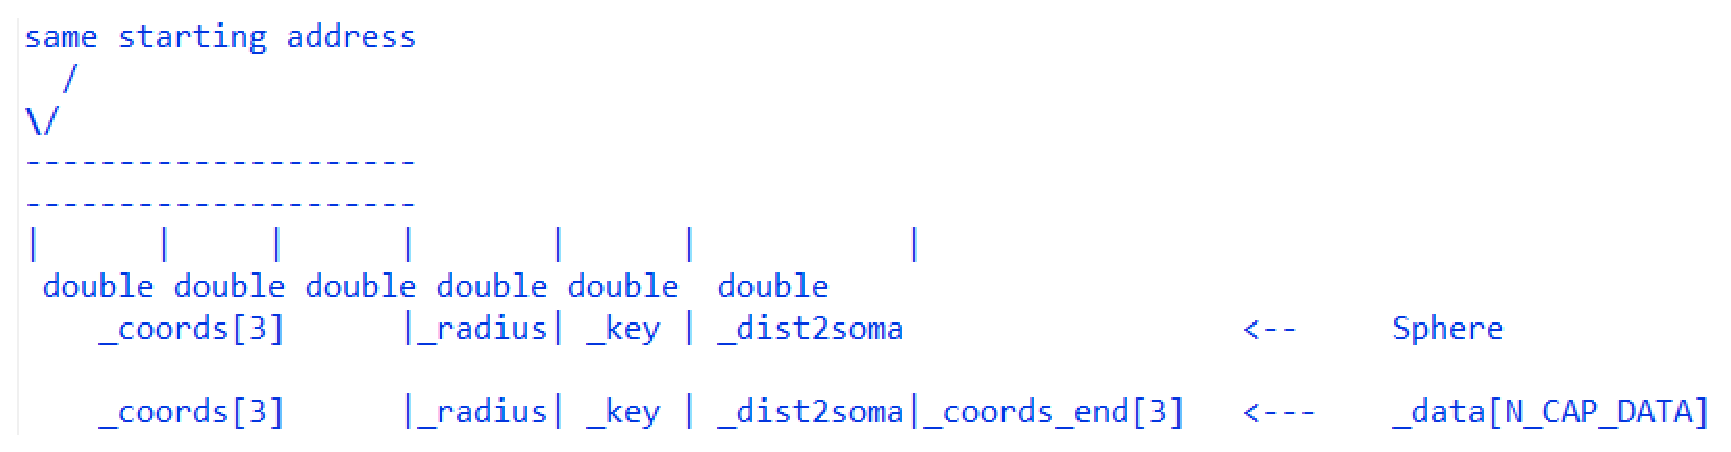
\includegraphics[height=2cm,
    angle=0]{./images/NTS_Capsule.eps}}
\caption{Capsule data structure}
\label{fig:NTS_Capsule}
\end{figure}


Code:
{\small
\begin{lstlisting}
#define N_SPHERE_DATA 6
#define N_CAP_DATA (N_SPHERE_DATA + 3)
#define CAP_END_COORD N_SPHERE_DATA

struct Sphere
{
  double _coords[3];
  double _radius;
  double _key;  //key_size_t
  double _dist2Soma;
};

class Capsule
{
public:
  void setKey(key_size_t key) {_capsuleData._sphere._key=key;}

private:
  union CapsuleData {
    Sphere _sphere;
    double _data[N_CAP_DATA];
  } _capsuleData;
 
  ComputeBranch* _branch;
  static SegmentDescriptor _segmentDescriptor;
  
}
\end{lstlisting}
}

\subsection{TissueSite}
\label{sec:TissueSite}

\begin{lstlisting}
class TissueSite: public Struct
{
public:

   double x;  // the coordinates
   double y;
   double z;
   double r; // and the radius
}
\end{lstlisting}

We use this to define a coordinate with a radius, i.e. forming a sphere, which
can be passed to the Probe TissueFunctor
(Sect.\ref{sec:TissueFunctor-as-probe-functor}) as a criteria for defining
which compartment get the current stimulus, i.e. for forming a current stimulus
to any compartments that have an intersection with this sphere.

The class is being used in files containing compartmental data
\verb!HodgkinHuxleyVoltage.C!, \verb!HodgkinHuxleyVoltageJunction.C!,
\verb!CaConcentration.C!, \verb!VoltageDisplay.C!, \verb!CalciumDisplay.C!, and
some generated files \verb!CG_...! related to the above files.




\subsection{TissueContext}
\label{sec:TissueContext}

A TissueContext holds all information required for the simulation of tissue in
an MPI environment (which is required to run TissueFunctor) via the
\verb!_neurons! data member and others. This information is generated during
TissueFunctor's constructor
(Sect.\ref{sec:TissueFunctor-how-it-works-underlying})
\begin{enumerate}
  \item ComputeBranch - Sect.\ref{sec:ComputeBranch}
  \item Capsule - Sect.\ref{sec:Capsule}:
  
  This Capsule* data is constructed from Segments* data in Tissue object
  (Sect.\ref{sec:Tissue})
\end{enumerate}
%{\small
\begin{lstlisting}
class TissueContext
{
  // VolumeDecomposition or other methods
  Decomposition* _decomposition; 

  int _nCapsules;
  Capsule* _capsules;  
  Capsule* _origin;
  TouchVector _touchVector;

  NeuronPartitioner* _neuronPartitioner; //created inside 
                              // TissueConnector:neuroDev()
                              
  Tissue* _tissue; //created inside TissueConnector:neuroDev()
        // = new Tissue(_size, _rank)
  
  RNG _touchSampler, _localSynapseGenerator;
  long _boundarySynapseGeneratorSeed, _localSynapseGeneratorSeed;

  // keeps track of all neuron in this computing node
  // neuron is uniquely identified via its index - an integer
  //    index is defined based on the order in tissue.txt file
  // each neuron has a list of branches (ComputeBranch)
  std::map<	unsigned int, std::vector<ComputeBranch*> > _neurons;

  // define the mapping from a branch (represented by ComputeBranch)
  //    to the vector of all centroid-points in that branch
  // a centroid-point is the representation of a number of Capsules
  //    that has the same value of the compartmental variable in the solver
  // a centroid-point is represented by CG_CompartmentDimension class
  //            which is (x,y,z,r,dist2soma)
  std::map<ComputeBranch*, std::vector<CG_CompartmentDimension*> >
      _branchDimensionsMap;
  
  // define the mapping from a branch
  //    to the data uniquely identified the branch (CG_BranchData*)
  //              which is (key,size)
  //      key  = a key formed by multiple fields that uniquely identify that
  //      branch
  //      size = # of compartments in that branch
  std::map<ComputeBranch*, CG_BranchData*> _branchBranchDataMap;
  
  // define the linkage between a single compartment (as a junction point)
  //         (from which the branching occurs)
  //    to a list of other compartments (that joint to the the same junction
  //    point)
  std::map<Capsule*, CG_CompartmentDimension*> _junctionDimensionMap;
  
  // define the linkage between a single compartment (as a junction point)
  //    to the branch to which it belongs
  std::map<Capsule*, CG_BranchData*> _junctionBranchDataMap;
  // define the mapping from a key (representing a branch)
  //    to the index of a capsule
  std::map<key_size_t, int> _firstPassCapsuleMap,
      _secondPassCapsuleMap;  // key to capsule index

  NeuroDevCommandLine _commandLine;
  
private:
  SegmentDescriptor _segmentDescriptor;
  bool _seeded;
  int _rank, _mpiSize;
}
\end{lstlisting}
%}

\subsection{-- setUpCapsules}
\label{sec:TissueContext-setUpCapsules()}

This is the method that convert data points from .swc files
(or Segments data structure from neuron growth) into Capsules data structure
(Sect.\ref{sec:Capsule}).

\begin{verbatim}
int TissueContext::setUpCapsules(int nCapsules, DetectionPass detectionPass,
                                 int rank, int maxComputeOrder)
{
  Capsule* capsEnd = _capsules + nCapsules;
  resetBranches();  // clean-up all existing data
  std::sort(_capsules, capsEnd);
  capsEnd = std::unique(_capsules, capsEnd);
  _nCapsules = capsEnd - _capsules;
  if (detectionPass != NOT_SET)  // there is available Capsule data structure
  {
    for (int sid = 0; sid < _nCapsules; ++sid)
    {
      addToCapsuleMap(_capsules[sid].getKey(), sid, detectionPass);
    }
  }
  setUpBranches(rank, maxComputeOrder);
  return _nCapsules;
}
\end{verbatim}


\subsection{TouchSpace: SynapseTouchSpace, DendriteTouchSpace, AlInTouchSpace,
ORTouchSpace, NonautapticTouchSpace}
\label{sec:TouchSpace}

This is a similar concept to SegmentSpace (Sect.\ref{sec:SegmentSpace}).
To define if a touch if formed between two capsules, here, the class tells if
a capsule (or two Capsules), based upon their keys
(Sect.\ref{sec:SegmentDescriptor}), falls into the given touchspace or not.
\begin{enumerate}
  \item SynapseTouchSpace - Sect.\ref{sec:SynapseTouchSpace}
  \item DendriteTouchSpace - Sect\ref{sec:DendriteTouchSpace}
  \item NonautapticTouchSpace - Sect.\ref{sec:NonautapticTouchSpace}
  \item NonautapticAxoDendriticTouchSpace - Sect.\ref{sec:NonautapticAxodendriticTouchSpace}
  \item AllInTouchSpace - Sect.\ref{sec:AllInTouchSpace}
\end{enumerate}
and
\begin{enumerate}
%   \item NOTTouchSpace 
%   \item ANDTouchSpace
  \item ORTouchSpace  - Sect.\ref{sec:ORTouchSpace}
\end{enumerate}

 The abstract class
\begin{verbatim}
class TouchSpace
{
   virtual ~TouchSpace() {}
   virtual bool isInSpace(double segKey)=0;
   virtual bool areInSpace(double segKey1, double segKey2)=0;
}
\end{verbatim}


\subsection{-- SynapseTouchSpace}
\label{sec:SynapseTouchSpace}

A SynapseTouchSpace can be either ELECTRICAL (bidirectional) or CHEMICAL
(directional)


Check
\begin{verbatim}
class SynapseTouchSpace : public TouchSpace
{
   enum SynapseType {ELECTRICAL, CHEMICAL};
   SynapseTouchSpace(SynapseType type,
		     Params* params,
		     bool autapses);
   bool isInSpace(double key);
   bool areInSpace(double key1, double key2);
private:
   SynapseType _type;
   Params _params;
   bool _autapses;
  SegmentDescriptor _segmentDescriptor;
}


bool SynapseTouchSpace::isInSpace(key_size_t key)
{ 
  bool rval=false;
  if (_type==ELECTRICAL) rval=_params.isElectricalSynapseTarget(key);
  else if(_type==CHEMICAL) rval=_params.isChemicalSynapseTarget(key);
  return rval;
}
\end{verbatim}
Check Params - Sect.\ref{sec:Params.cxx}.

%  Ask James what is _autapses?
% ANSWER:  autapse is a touch form by the axon and dendrite of the same neuron

\subsection{-- DendriteTouchSpace}
\label{sec:DendriteTouchSpace}

The Capsules instance that is in soma, apical dendrite or basal
dendrite.

\begin{verbatim}
bool DendriteTouchSpace::isInSpace(key_size_t segKey1)
{
  return (_segmentDescriptor.getBranchType(segKey1) == 0 ||
	  _segmentDescriptor.getBranchType(segKey1) == 2 || 
	  _segmentDescriptor.getBranchType(segKey1) == 3 );
}
\end{verbatim}

\subsection{-- NonautapticTouchSpace}
\label{sec:NonautapticTouchSpace}

The two Capsules instances that are not from the same neuron.

\begin{verbatim}
bool NonautapticTouchSpace::areInSpace(key_size_t segKey1, key_size_t segKey2)
{
  return ( _segmentDescriptor.getNeuronIndex(segKey1)!= 
	   _segmentDescriptor.getNeuronIndex(segKey2) );
}
\end{verbatim}

\subsection{-- NonautapticAxodendriticTouchSpace}
\label{sec:NonautapticAxodendriticTouchSpace}

A Capsule instance that is part of the axon; or
Two Capsule instances not from the same neuron, one from the axon, and the other
two must be either apical dendrite or basal dendrite.

\begin{verbatim}
bool NonautapticAxodendriticTouchSpace::isInSpace(key_size_t segKey1)
{
  return (_segmentDescriptor.getBranchType(segKey1) == 1);
}

bool NonautapticAxodendriticTouchSpace::areInSpace(key_size_t segKey1,
                                                   key_size_t segKey2)
{
  return ((_segmentDescriptor.getNeuronIndex(segKey1) !=
           _segmentDescriptor.getNeuronIndex(segKey2)) &&

          (_segmentDescriptor.getBranchType(segKey1) == 1) &&

          (_segmentDescriptor.getBranchType(segKey2) == 2 ||
           _segmentDescriptor.getBranchType(segKey2) == 3));
}
\end{verbatim}

\subsection{-- ORTouchSpace}
\label{sec:ORTouchSpace}

\begin{verbatim}
class ORTouchSpace : public TouchSpace
{
 private:
   TouchSpace* _touchSpace1;
   TouchSpace* _touchSpace2;
}
\end{verbatim}

\subsection{-- AllInTouchSpace}
\label{sec:AllInTouchSpace}


\subsection{Touch}
\label{sec:Touch}

\begin{verbatim}
class Touch
{

private:
// 0 = key1  (key of capsule 1)
// 1 = key2  (key of capsule 2)
// 3 = prop1  (the ratio on capsule1 at which we can find the point of shorttest distance
// 4 = prop2 
// 5 = the value of the shortest distance between capsule1 and capsule2
 double _touch_data[N_TOUCH_DATA];
}
\end{verbatim}

\subsection{TouchVector}
\label{sec:TouchVector}

A TouchVector holds data as Touch instances (Sect.\ref{sec:Touch})
\begin{verbatim}
typedef BlockVector<Touch>::Index TouchIndex;

class TouchVector : public BlockVector<Touch> {
 private:
  std::map<int, std::list<TouchIndex> > _touchMap;
}
\end{verbatim}


Data in one block represents the data from one MPI-process (Check
Sect.\ref{sec:detectTouches()}).

\begin{verbatim}
  TouchVector& touchVector = _threadUserData->_touchVectors[threadID];
\end{verbatim}

\begin{lstlisting}
// a vector of 'Touch' is organized
// in the form of multiple blocks of 'Touch'
// data in one block is guaranteed to be contiguous

// a vector of pointer to different blocks of data
template<typename T> 
class BlockVector {
 private:
  int fieldDefaultBlockSize;
  std::vector<Block<T> *> fieldBlocks;
 public:
}

// a contiguous block of data of type 'T'
template<typename T> 
class Block {
 private:
  int fieldSize;
  int fieldCount;
  T *fieldValues;
 public:
}
\end{lstlisting}

\subsection{TouchAnalyzer}
\label{sec:TouchAnalyzer}


\begin{verbatim}
class TouchAnalyzer : public Sender, public Receiver
{
}
\end{verbatim}

\subsection{TouchAggregator}
\label{sec:TouchAggregator}

This class combines touches detected by the current MPI process, and touches
sent to it from other MPI processes - such touches are chosen by the
TouchDetectTissueSlicer (Sect.\ref{sec:TouchDetectTissueSlicer}).

\begin{verbatim}
class TouchAggregator : public Receiver
{

}
\end{verbatim}

\subsection{TouchDetector}
\label{sec:TouchDetector}

A TouchDetector object, once created needs a few information
\begin{enumerate}
  \item the 'rank' to know what capsules belong to that MPI process
  
  \item the 'nSlicers' to know
  
  \item the 'nTouchDetectors' to know
  
  \item the 'appositionRate' : the prob. for a touch is formed
  
  \item the 'decomposition' 
  
  \item the 'detectionTouchSpace': the  criteria for two capsules 
  to be able to form a touch
  
  \item the 'communicateTouchSpace': can be NULL (0)
  
  \item the 'neuronPartitioner' 
  
  \item the 'tissueContext'
  
  \item the 'params'
\end{enumerate}

{\tiny
\begin{verbatim}
class TouchDetector :  public Sender, public Receiver
{
     class TDSegment
     {
      public:
       double seg[N_TD_DATA];
       double* getBeginCoords() {return &seg[TD_BEGIN_COORDS];}
       double getRadius() {return seg[TD_RADIUS];}
       double getKey() const {return seg[TD_KEY];}
       double* getEndCoords() {return &seg[TD_END_COORDS];}
       bool operator<(const TDSegment& s1) const;
       bool operator==(const TDSegment& s1) const;
     };

   private:

     int _numberOfSenders;
     int _numberOfReceivers;
     int _rank;
     int _nSlicers;
     int _nTouchDetectors;
     int _maxComputeOrder;
     int _nThreads;
     ThreadUserData* _threadUserData;

     double _appositionRate;
     Decomposition** _decomposition;
     TouchSpace* _detectionTouchSpace;
     TouchSpace* _communicateTouchSpace;
     NeuronPartitioner* _neuronPartitioner;
     Params* _params;
     bool _writeToFile;
		 
     long long _connectionCount;
     TouchAnalyzer* _touchAnalyzer;

     // Receive Phase 0: ALLTOALL
     int *_segmentsPerSender; 		    // recvbuf
     int _numberOfInts;                     // recvcount
     MPI_Datatype _typeInt;                 // recvtype
        
     // Receive Phase 1: ALLTOALLW
     Capsule** _capsules;         // ptr to recvbuf array
     TouchVector* _touchVector;
     TouchVector _initialTouchVector;

     int* _segmentCounts;         // recvcount
     int* _segmentDispls;         // recvDispls
     MPI_Datatype* _typeSegments; // recvtype
     int _segmentDataSize;
     int _numberOfCapsules;
     int _previousPhase1RecvBufSize;
     
     // Send Phase 0: ALLTOALL
     int *_touchesPerReceiver;
     
     // Send Phase 1: ALLTOALLW
     Touch* _touchOrigin;
     int* _touchCounts;
     int* _touchDispls;
     MPI_Datatype* _typeTouches;
     double* _sendBuf;
     int _sendBufSize;
     int _maxNumTouches;
     int* _touchBlockLengths;
     MPI_Aint* _touchBlockDisplacements;

     bool _unique, _resetBufferSize, _receiveAtBufferOffset;
     TissueContext* _tissueContext;
     TissueContext::DetectionPass _detectionPass;
     std::string _experimentName;

}
\end{verbatim}
}

Once we have the object, we can perform touch detection
which goes through a set of passes
\begin{enumerate}
  \item \verb!TissueContext::FIRST_PASS!
  
  \item setUpCapsules(): convert Segments into Capsules (Sect.\ref{sec:setUpCapsules()})
  
  \item detectTouches(): detect touches between Capsules (Sect.\ref{sec:detectTouches()}) 

  \item write the data out:
  
\begin{verbatim}
outTouches_%s_%d.bin     (_experimentName, _rank)
\end{verbatim}
  
\end{enumerate}


C++ CODE:
\begin{lstlisting}
void TouchDetector::finalizeReceive(int receiveCycle, int receivePhase)
{
	assert(receiveCycle==0);
	switch (receivePhase) {
		case 1 :
			if (_tissueContext==0) {
				setUpCapsules();
				detectTouches();
			}
	}
}

\end{lstlisting}

\subsection{-- setUpCapsules()}
\label{sec:setUpCapsules()}

It indeeds use TissueContext's \verb!setUpCapsules()! method to do the job
(Sect.\ref{sec:TissueContext-setUpCapsules()})

\begin{verbatim}
// NOTE: _segmentDataSize = # of capsules (derived from # of segments)

void TouchDetector::setUpCapsules() {
  if (_tissueContext) {
    _numberOfCapsules = _segmentDataSize = _tissueContext->setUpCapsules(
        _segmentDataSize, _detectionPass, _rank, _maxComputeOrder);
  } else {
    Capsule* caps = *_capsules, *capsEnd = caps + _segmentDataSize;
    std::sort(caps, capsEnd);
    capsEnd = std::unique(caps, capsEnd);
    _segmentDataSize = _numberOfCapsules = capsEnd - caps;
  }
}
\end{verbatim}



\subsection{-- detectTouches()}
\label{sec:detectTouches()}

\verb!TouchDetector::detectTouches()! loops through the list of Capsules, and
call \verb!doWork()! to find another Capsule that 'touch' the given Capsule.
A touch is formed if all conditions satisfy
\begin{enumerate}
  \item Two capsules belong to the same space (Sect.\ref{sec:TouchSpace})
  
  \item The shortest distance between any two points on the two capsules falls
  within the given range, i.e. given radius $r$ ($\mum$)

NOTE: New strategy to avoid touch forming between one capsule A with 2 adjacent
capsules B and Bparent and Bchild on the one branch
\begin{itemize}
  \item Find the distance between A and Bparent; if the distance between
  (A,Bparent) is shorter than between (A,B) then let the touch to be formed
  between (A,Bparent)
  
  \item Find the distance between A and Bchild; if the distance between
  (A,Bchild) is shorter than between (A,B) then let the touch to be formed between (A,Bchild)
\end{itemize}

  \item The probability for a touch to form is met (by comparing a generated
  pseudo-random number with a given probability value)
\end{enumerate}


Each MPI process hold the all data via \verb!_threadUserData!
(Sect.\ref{sec:ThreadUserData}).

A Touch is created if 3 conditions meet:
\begin{enumerate}
  \item two Capsules fall into the same TouchSpace (Sect.\ref{sec:TouchSpace})
  \item the distance between thems falls into the range of distance
  \item generate a random value, and this value smaller than the probability
  of generating the touch
\end{enumerate}


\begin{verbatim}
for(int sid=0; sid<_numberOfCapsules; ++sid) {
    // here multi-threads is not used, i.e. each MPI process has 1 thread only
    doWork(0, sid, _threadUserData, 0);
}//for (; sid<_nCapsules...
\end{verbatim}

% which loops through every capsule, represented by \verb!sid! (index), and indeed
% calls \verb!TouchDetector::doWork()! 
% TODO: NTS multi-thread for touch detection	
% \begin{verbatim}
% for(int sid=0; sid<_numberOfCapsules; ++sid) {
%     for (int thread=0; thread< _numThreads;, ++thread)
%        doWork(thread, sid, _threadUserData, 0);
% }//for (; sid<_nCapsules...
% \end{verbatim}

C++ CODE: doWork()
{\small
\begin{lstlisting}
void TouchDetector::doWork ( ... ) 
{
// loop through all capsules
for(int sid2=0; sid2<_numberOfCapsules; ++sid2)
    // the rate of forming a capsule for a given branch (-a option)
   if ( _appositionRate>=1.0 || drandom(rng)<_appositionRate) 
{
 //
    double s1Key = caps[sid].getKey();
    double s2Key = caps[sid2].getKey();
    
    double* s1begin = caps[sid].getBeginCoordinates();
    double* s1end = caps[sid].getEndCoordinates();
    //original formula:   s1Ar =
    caps[sid].getRadius()+params->getRadius(s1Key);j //new
    s1Ar = (params->getRadius(s1Key)>=0) ? caps[sid].getRadius()+params->getRadius(s1Key) : 0;
   
    //check the keys of the two capsules
    // are in the samespace, i.e. the first condition for touch formation
    if (detectionTouchSpace->areInSpace(s1Key, s2Key)) {

      // the next condition would the distance (within a sphere of a given
      // radius
      // NOTE: We need to discritize the capsule into
      //       a series of points
      // i.e. we have two set of points
      //   and find the pair of points (p_set1, p_set2) 
      //   with the nearest distance 
      //   and finally check with the given radius above
      ...
      
    }
}
}
\end{lstlisting}
}



\subsection{GlomeruliDetector: InferiorOliveGlomeruliDetector}
\label{sec:GlomeruliDetector}
\label{sec:InferiorOliveGlomeruliDetector}




\section{New classes for kinetic/dynamic modeling a neuron}

The mdl file \verb!HodgkinHuxley.mdl! define commonly used interface
(Sect.\ref{sec:HodgkinHuxley.mdl}).

In order to help solving the compartment variable or variable
that has diffusion (e.g. Voltage, Calcium), we map them onto 
the neuron tree in the form of two types branches

First, understand a ComputeBranch concept (Sect.\ref{sec:ComputeBranch}). 
A ComputeBranch, depending its computeOrder, can connect to either
\begin{verbatim}
    distal-end                   proximal-end
BackwardSolverPoint      |    
               if the 0 <= computeOrder < MAX_COMPUTE_ORDER    
                         |    FordwardSolverPoint 
           --> if the 0 < computeOrder <= MAX_COMPUTE_ORDER
   EndPoint                    
   |
   Junction
   |
   JunctionPoint
   |
   CompartmentVar
         --> if computeOrder == MAX_COMPUTE_ORDER
                         |    
                                    EndPoint                    
                                    |
                                    Junction
                                    |
                                    JunctionPoint
                                    |
                                    CompartmentVar
         --> if computeOrder == 0
            
\end{verbatim}


% \begin{enumerate}
%   \item ComputeBranch that from branching-point to a cut-point:
%   
%   The distal-end faces the ForwardSolverPoint, and 
%   proximal-end faces the 
%   
%   regular
%   compartment at computeOrder
%   
%   
% \end{enumerate}

\begin{enumerate}
  \item regular branch, e.g. HodgkinHuxleyVoltage (Sect.\ref{sec:regular-branch-neuron})
  
  To support the solver, at each end, we needs 2 end-points, e.g.
  VoltageEndPoint - Sect\ref{sec:HodgkinHuxleyVoltage.mdl} maps to either ends
  depends on 'distalEnd' or 'proximalEnd' is used in setPointers() function.
  
  \item junction branch, e.g.  HodgkinHuxleyVoltageJunction
  (Sect.\ref{sec:junction-branch-neuron})

  To support the solver, at each end, we needs 2 end-points, e.g.
  VoltageJunctionPoint - Sect\ref{sec:HodgkinHuxleyVoltageJunction.mdl} maps to either
  ends depends on 'distalEnd' or 'proximalEnd' is used in setPointers()
  function. Here, there is only one input from proximal end, but many input from
  distal ends.

\end{enumerate}

\subsection{Understand branch solver}

The file \verb!BranchSolver.mdl! contains Interface and Node that will be used
to handle the solving of voltage diffusion (and any thing, e.g. calcium)
diffusion across one branch to another at the level of ComputeBranch
(Sect.\ref{sec:ComputeBranch})

\begin{verbatim}
if (br->_parent)
{  // check proximal-end
					   //if	it connects to a proximal-ComputeBranch
     if (computeOrder==0) 
     {  // start to have an explicit junction at proximal-end 
        // connect (1) compartment to endpoint 
		//         (2) endpoint to explicit junction
		//         (3) explicit junction to junction point,
		//         (4) junction point to compartment 
     }
     else
     {  // implicit junction at proximal-end
		// connect (1) compartment to forward solver 
     }
}


if (br->_daughters.size() > 0)
{//check distal-end 
			// if the ComputeBranch connects to other distal-ComputeBranch
            // get to all instances of the associated diffusible nodetype (e.g.
            //     Voltage, Calcium)
            //     at one ComputeBranch
    if (computeOrder==MAX_COMPUTE_ORDER-1)
     { //start to have an explicit junction on distal-end
						   // connect (1) compartment to endpoint 
						   //         (2) endpoint to explicit junction
						   //         (3) explicit junction to junction point,
						   //         (4) junction point to compartment 
    }
    else
    {  // implicit junction at distal-end
	   // connect (1) compartment to backward solver 
    }
}
\end{verbatim}

\subsection{-- regular branch}
\label{sec:regular-branch-neuron}

For each regular branch, there will be two associated endpoints that reference
to the proper voltage/dimension value from the compartment of \verb!distalEnd!
or \verb!proximalEnd!, accordingly.

Example: VoltageEndPoint
\begin{verbatim}
void VoltageEndPoint::setPointers(const String& CG_direction, const String& CG_component, 
        NodeDescriptor* CG_node, Edge* CG_edge, VariableDescriptor* CG_variable, 
        Constant* CG_constant, CG_VoltageEndPointInAttrPSet* CG_inAttrPset, 
        CG_VoltageEndPointOutAttrPSet* CG_outAttrPset) 
{
  if (CG_inAttrPset->identifier=="distalEnd") {
    assert(getSharedMembers().voltageConnect);
    assert(getSharedMembers().voltageConnect->size()>0);    
    voltage = &((*(getSharedMembers().voltageConnect))[0]);
    assert(getSharedMembers().dimensionsConnect);
    assert(getSharedMembers().dimensionsConnect->size()>0);    
    dimension = (*(getSharedMembers().dimensionsConnect))[0];    
  }
  else if (CG_inAttrPset->identifier=="proximalEnd") {
    assert(getSharedMembers().voltageConnect);
    assert(getSharedMembers().voltageConnect->size()>0);    
    voltage = &((*(getSharedMembers().voltageConnect))[getSharedMembers().voltageConnect->size()-1]);
    assert(getSharedMembers().dimensionsConnect);
    assert(getSharedMembers().dimensionsConnect->size()>0);    
    dimension = (*(getSharedMembers().dimensionsConnect))[getSharedMembers().dimensionsConnect->size()-1];
  }
  else {
    std::cerr<<"Warning! Unrecognized input identifier on VoltageEndPoint!"<<std::endl;
  }
}

\end{verbatim}

\subsection{-- junction branch}
\label{sec:junction-branch-neuron}

To treat every thing as branch, there are special cases that we categorize them
as junction branch:
\begin{itemize}
  \item a soma with multiple branches
  
  In terms of surface area:
  \begin{verbatim}
  surface area = soma-spherical-surface-area -
                 sum(cross-sectional-area-of-branches)
  \end{verbatim}
  
  \item a dendritic junction with multiple branches

  In terms of surface area:
  \begin{verbatim}
  surface area = sum(half-surface-area of all cylinder)
  \end{verbatim}
\end{itemize}


For each junction branch, they are assumed a isopotential, i.e. all compartments
in that junction branch references to the same voltage of the first compartment 
\begin{verbatim}
void VoltageJunctionPoint::setPointers(const String& CG_direction, 
         const String& CG_component, NodeDescriptor* CG_node, Edge* CG_edge,
         VariableDescriptor* CG_variable, Constant* CG_constant,
         CG_VoltageJunctionPointInAttrPSet* CG_inAttrPset,
         CG_VoltageJunctionPointOutAttrPSet* CG_outAttrPset)
{
  assert(getSharedMembers().voltageConnect);
  assert(getSharedMembers().voltageConnect->size()==1);    
  assert(getSharedMembers().dimensionsConnect);
  assert(getSharedMembers().dimensionsConnect->size()==1);    
  voltage = &((*(getSharedMembers().voltageConnect))[0]);
  dimension = (*(getSharedMembers().dimensionsConnect))[0];
}
\end{verbatim}


\textcolor{red}{Boundary condition}, e.g. Voltage initialize:
{\small
\begin{lstlisting}
#define isProximalCase0 (proximalDimension==0) // no flux boundary condition
#define isProximalCase1 (proximalJunction==0 && proximalDimension!=0) // connected to proximal cut 
                                 //or branch point for implicit solve
#define isProximalCase2 (proximalJunction) // connected to proximal junction

#define isDistalCase0 \
  (distalDimensions.size() == 0)  // no flux boundary condition
#define isDistalCase1 \
  (distalAiis.size() == 1)  // connected to distal cut point for implicit solve
#define isDistalCase2        \
  (distalAiis.size() == 0 && \
   distalInputs.size() == 1)  // connected to distal junction
#define isDistalCase3  \
  (distalAiis.size() > \
   1)  // connected to distal branch point for implicit solve

 if (isProximalCase2) assert(computeOrder == 0);
 if (isDistalCase2) assert(computeOrder == MAX_COMPUTE_ORDER);

\end{lstlisting}
}

\subsection{Supporting interfaces: HodgkinHuxley.mdl}
\label{sec:HodgkinHuxley.mdl}

NOTE: There are some inconsistence in naming
\begin{verbatim}
// in Interface with ...ArrayProducer{}
  - some use ..Array; as suffix in data member  
  - some use ..s;     as suffix in data member
\end{verbatim}

This file contains most interfaces we need for data exchange (data
communication). \textcolor{red}{IMPORTANT: Currently we use float, but it can be
mapped to 64-bit by using the compiler option}.

{\tiny
\begin{verbatim}
// For Variable injecting current into the cell for stimulus purpose
Interface CurrentProducer {  float * current;}
Interface CurrentArrayProducer { float[]* current;}

// For Node producing calcium current
Interface CaCurrentProducer { float * current;}
Interface CaCurrentArrayProducer { ...}

// This interface can be used for any Node as a channel that can has 
// a reversal potential component
//  NodeType NaTChannel
//  NodeType CahChannel 
Interface ReversialPotentialProducer { float * reversalPotential;}
Interface ReversialPotentialArrayProducer { ...}

// This interface can be used for any Node as a channel that can has a
// conductance component
Interface ConductanceProducer{ float * conductance;}
Interface ConductanceArrayProducer {...}

// This interface can be used for any Node as a membrane (e.g.
//  HodgkinHuxleyVoltage) that has a voltage component
Interface VoltageProducer {float * voltage;}
Interface VoltageArrayProducer { ...};

// This interface can be used for any Node as a component (e.g.
//  CaER, CaMyo)
// that has [Ca] component
Interface CaConcentrationProducer { float * Ca;}
Interface CaConcentrationArrayProducer { float[] * Ca;}

// This interface is used for Node 
//   as NMDAReceptor in which [Ketamine] affect the gating as a blocker
//   as ExtracellularMedium in which [Ketamine] changess
Interface KetamineConcentrationProducer { float * K;};


// Currently, Mg and Na are asssumed unchanged
Interface MgConcentrationProducer { float * Mg;}
Interface NaConcentrationProducer { float * Na;};
Interface KConcentrationProducer { float * K;};



// Interfaces for plasticity or weight of connections
Interface WeightProducer { float * W;}
Interface PlasticityProducer{ float * w;}

Interface PlasticityToggleProducer{ int* plasticityToggle;}

// Temperature 
// used by any Node that requires Temperature in the calculation, e.g. 
//  NodeType of channels
Interface TemperatureProducer{ float * T;}

//  not sure what it's for
Interface IndexProducer { int* index;}

// This interface is used for Node that make use of the 
// surface area of the branch in their calculation, e.g. 
//  total ionic current passing a surface area
Interface SurfaceAreaProducer { float* surfaceArea;}

// This interface is used for Node that make use of the 
// surface area between two adjacent branches of the same NodeType
// to calculate the diffusion 
Interface ConnectionSurfaceAreaProducer { float* surfaceArea;}


// This interface is used for Constant
// keeping data that are supposed to be fixed during the whole simulation
Constant ExtracellularMedium Implements NaConcentrationProducer, KConcentrationProducer, 
                                        CaConcentrationProducer,
                                        MgConcentrationProducer,
                                        TemperatureProducer, 
                                        KetamineProducer {
  float Na; // intracellular concetrations expressed by ion name alone
  float K;
  float Ca;
  float Mg;
  float T;
  float Ketamine;
  NaConcentrationProducer.Na << &Na;
  KConcentrationProducer.K << &K;
  CaConcentrationProducer.Ca << &Ca;
  MgConcentrationProducer.Mg << &Mg;
  TemperatureProducer.T << &T;
  KetamineProducer.Ketamine << &Ketamine;
}
\end{verbatim}
}


\subsection{ExtraCellular environment}
\label{sec:NTS-extracellular-environment}

In the original NTS, extracellular environment comprised certain ion
concentrations (Na, K, Ca, \ce{Mg2+}, Ketamine, and temperature), which is
defined in Sect.\ref{sec:HodgkinHuxley.mdl}.

To support more complicated scenario, e.g. interacting with vasculature, a
replacement is used


\subsection{Classes for a 'branching' calculation variable, e.g. Voltage}



% \begin{verbatim}
% HodgkinHuxleyVoltage.mdl
% HodgkinHuxleyVoltageJunction.mdl
% \end{verbatim}

\subsection{- Node: HodgkinHuxleyVoltage, VoltageEndPoint}
\label{sec:HodgkinHuxleyVoltage.mdl}
\label{sec:HodgkinHuxleyVoltage-mdl-code}

HodgkinHuxleyVoltage.mdl define \verb!HodgkinHuxleyVoltage! node, and another
node HodgkinHuxleyVoltageEndPoint that is important for solving the voltage.

defines (Sect.\ref{sec:MDL-generated-classes} discusses the generated C++
classes) 

{\small
\begin{lstlisting}
Node HodgkinHuxleyVoltage Implements 
        // a comma-separated list of Interfaces
        // defining the input data
        //          the output data
        VoltageArrayProducer,  // output for any other uses 
        
        NaConcentrationProducer, // input for calculating voltage
        KConcentrationProducer, // input for calculating voltage
        
        SolutionArrayProducer,  // these below are for solver purpose
        DimensionArrayProducer,
        BranchDataProducer,
        ForwardSolutionArrayProducer
        
{ 
 // then we define one or many internal data member
 // which is typically in the form of an array
 float [] Vcur; //current-value
 float [] Vnew; //next-value

 // then define shared data among the different instances of this Node
 // which is typically a scalar pointer
 Shared {
   float * deltaT;
   float * Na;
 }
 

 // output
 // the define which data member maps to which data member in which interface
 // use << to indicate that the Interface hold the output data
 VoltageArrayProducer.voltageArray << &Vnew;
 NaConcentrationProducer.Na << &Shared.Na;
 
 BranchDataProducer.branchData << branchData;
 ForwardSolutionArrayProducer.AiiArray << &Aii;  //NOTE: Aii is the pointer 
 ForwardSolutionArrayProducer.AipArray << &Aip;
 ForwardSolutionArrayProducer.RHSArray << &RHS;

 // The kernel to initialize the data member
 InitPhase initializeVoltage;

 // In order to update the data member, we need to choose the solver, which is 
 // implemented as a set of kernels in RuntimePhase
 // Here the method allows upto 7 order
 // the higher the order the more accurate ???
  #if MAX_COMPUTE_ORDER>0
  RuntimePhase forwardSolve1, backwardSolve1; 
  #endif
  #if MAX_COMPUTE_ORDER>1
  RuntimePhase forwardSolve2, backwardSolve2; 
  #endif
  #if MAX_COMPUTE_ORDER>2
  RuntimePhase forwardSolve3, backwardSolve3; 
  #endif
  #if MAX_COMPUTE_ORDER>3
  RuntimePhase forwardSolve4, backwardSolve4; 
  #endif
  #if MAX_COMPUTE_ORDER>4
  RuntimePhase forwardSolve5, backwardSolve5; 
  #endif
  #if MAX_COMPUTE_ORDER>5
  RuntimePhase forwardSolve6, backwardSolve6; 
  #endif
  #if MAX_COMPUTE_ORDER>6
  RuntimePhase forwardSolve7, backwardSolve7; 
  #endif
  // The minimum
  RuntimePhase solve, finish;
 
  // user-defined kernel, i.e. those will be called by the different
  // phases' kernels
  UserFunction setReceptorCurrent, setInjectedCurrent, setProximalJunction;
  
  // user-defined kernel, but is supposed to return 'bool' type
  PredicateFunction confirmUniqueDeltaT;
 
 
  InAttrPset {
     string      identifier;
     TissueSite  site;
     int         idx;
  }
  
  // input, i.e. read data from other Nodes/Constant/Variable
  // use >> to indicate that we read the data from Interface
  Connection Pre Constant (PSet.identifier == ``dimension'')
                          Expects DimensionProducer { 
     DimensionProducer.dimension >> dimensions;  // MDL: DimensionStruct* [] dimensions;
  }
}
\end{lstlisting}
}
NOTE: TissueSite (Sect.\ref{sec:TissueSite}).

% TODO: Ask James why branchData is being read-in and write-out in
% HodgkinHuxleyVoltage Node through the same Interface

NOTE: Two important data for a 'CompartmentalComponent' Node in TissueFunctor
requires
\begin{verbatim}
  DimensionStruct* [] dimensions;
  BranchDataStruct* branchData;

  DimensionArrayProducer.dimensionArray << &dimensions;
  BranchDataProducer.branchData << branchData;
\end{verbatim}
DimensionStruct - Sect.\ref{sec:DimensionStruct}, and BranchDataStruct
(Sect.\ref{sec:BranchDataStruct}).


% TODO: Ask James what is the purpose of some data in HodgkinHuxleyVoltage
%       Aii, Aip, Aim, RHS, Aij

% TODO: Ask James why some places in Shared data does not use pointer
%         - float * deltaT;
%           float Ra;

% TODO: Ask James if the higher the order, the more accurate of the sover?

% TODO: Ask James what is the purpose of PredicateFunction keyword in MDL
%    ANSWER: To define a boolean user-defined function


\subsection{- Node: HodgkinHuxleyVoltageJunction,
VoltageJunctionPoint}
\label{sec:HodgkinHuxleyVoltageJunction.mdl}

For each junction variable (touch between two different branches, one from one
neuron - one from another), we need ???
%HodgkinHuxleyVoltageJunction.mdl

defines
\begin{lstlisting}

\end{lstlisting}


% \subsection{Node: VoltageEndPoint}
% 
% HodgkinHuxleyVoltage.mdl


\subsection{- Node: BranchSolver.mdl}
\label{sec:BranchSolver.mdl}

The file \verb!BranchSolver.mdl! contains Interface and Node that will be used
to handle the solving of voltage diffusion (and any thing, e.g. calcium,
diffusion) across one branch to another.

% TODO: Ask James what is the meaning of 'size' here?

% TODO: Ask James - a pointer to an array of pointer - data may be scattered
\begin{enumerate}
  
  \item BranchDataStruct:  \label{sec:BranchDataStruct}
  
\end{enumerate}
\begin{lstlisting}

// 
Interface DimensionProducer { DimensionStruct* dimension;}
Interface DimensionArrayProducer{ DimensionStruct* []* dimensionArray;}

// each point (along the branch/compartment)
// is uniquely identified using these information
Struct DimensionStruct {
  float x; 
  float y;
  float z;
  float r;
  float dist2soma;
}
\end{lstlisting}
% TODO: Ask James what is the usage of 'dist2soma' here,
% as it may not convey much meaningful information if it is the Eucledian
% distance



\subsection{* BranchData (branch type)}
\label{sec:BranchDataStruct}


\begin{verbatim}
// A branch in the neuron tree is uniquely identified by its key
Struct BranchDataStruct {
  double key; 
  //key_size_t key; // bit-mask to uniquely identify the branch 
  int size;  // num. compartments on that branch
}
Interface BranchDataProducer{ BranchDataStruct* branchdata;}

//Struct BranchDataStruct {
//  unsigned size;
//}

Interface BranchDataProducer{ BranchDataStruct* }
Interface BranchDataArrayProducer{ BranchDataStruct*[] * }

Constant BranchData Implements BranchDataProducer {
  BranchDataStruct branchData;
  BranchDataProducer.branchData << &branchData; //pass reference
}
\end{verbatim}
%TODO: NTS GPU PORT - NOTE the data are not contiguous 

\subsection{*ForwardSolution + BackwardSolution}

\begin{verbatim}
Interface ForwardSolutionProducer {
   dyn_var_t* Aii;
              Aip;
              RHS; //right-hand side
}

Node ForwardSolverPoint1 Implements ForwardSolutionProducer, DimensionProducer
{

}

Node BackwardSolverPoint0 Implements SolutionProducer, DimensionProducer
{
   dyn_var_t * solution;
   DimensionStruct * dimension;
   Shared {
      dyn_var_t * 
   }
}
\end{verbatim}

We can have maximum 7 compute-order, i.e. the whole branching tree is divided
into groups of every 7 compute-order. The solving in these groups are
independent; and in each group, the solving order is given as
\begin{verbatim}
updateNMDAPlasticity
solveChannels
predictJunction
forwardSolve7 
forwardSolve6 
...
forwardSolve1
solve
backwardSolve1
...
backwardSolve7
correctJunction
finish
\end{verbatim}
The minimum is 
\begin{verbatim}
updateNMDAPlasticity
solveChannels
predictJunction
solve
correctJunction
finish
\end{verbatim}


\subsection{* DimensionStruct (compartment coordinate)}
\label{sec:DimensionStruct}

It is assumed that all calculation, e.g. voltage value, injected current,
receptor currents, are solved at each compartment at the central point of it.
A Compartment (Sect.\ref{sec:compartment-in-neuron}) is thus represened as a
DimensionStruct, i.e. a structure representing a single point along the
dendritic tree which include coordinate (x,y,z), the radius of the cable (r),
and the distance from that central point of the compartment to the soma along
the dendrite (dist2soma) path.


{\bf VERSION 1}:
\begin{itemize}
  \item regular compartment: (x,y,z) the averge between first capsule's first
  coord and last capsule's last coord - thus ignore the geometry of
  multiple-capsule compartment
  
  By using ceiling division - there is a chance that there are 5-capsule
  compartment, and only 1-capsule compartment -- giving large bias in size
  
  radius (r) = the average of radius of all capsules
  
  dist2soma = fiber-along distance to soma from the first capsule's first coord
  
  \item junction compartment: (x,y,z) the coord of the last capsule's second
  coord in the branch where junction start
  
  radius (r) = the radius of the capsule above
  
  dist2soma = fiber-along distance to soma from the capsule above's first coord
  
\end{itemize}

{\bf VERSION 2}:
\begin{itemize}
  \item regular compartment: (x,y,z) removed
  
  radius (r) = the average of radius of all capsules
  
  dist2soma = fiber-along distance to soma from the first capsule's first coord
  (subtract the area taken by the explicit junction)
  
  surface-area = take into accounts compartment facing junction and soma
  
  \item junction compartment: (x,y,z) removed
  
  radius (r) = the radius of the capsule on the branch starting junction
  
  dist2soma = fiber-along distance to soma from the capsule above's first coord
  
  surface-area = take sum of half of surface area from all capsules of junction
   
\end{itemize}

\begin{verbatim}
Struct DimensionStruct {
  float x;
        y;
        z;
        r;
        dist2soma;
}

Interface DimensionProducer { DimensionStruct*}
Interface DimensionArrayProducer { DimensionStruct* [] * };

// become CG_CompartmentDimension class
Constant CompartmentDimension Implements DimensionProducer {
  DimensionStruct dimension;
  DimensionProducer.dimension << &dimension;
}
\end{verbatim}
%TODO: NTS GPU PORT - NOTE the data are not contiguous 


\subsection{* DiffusionSolver: Voltage}

We need to create 2 node types: \verb!HodgkinHuxleyVoltage! and 
\verb!VoltageEndPoint!. 
\begin{itemize}
  \item HodgkinHuxleyVoltage: 
  \item The VoltageEndPoint is the class that is used to reference to the last
  endpoint
\end{itemize} 



\subsection{Class for an ion channel, e.g. NaChannel}
\label{sec:NaChannel.mdl}

For each receptor variable, we need ???


{\small
\begin{verbatim}
Node NaChannel Implements
                 ConductanceArrayProducer,
                 ReversalPotentialArrayProducer,
                 BranchDataProducer
{
   float [] m;
   float [] h;
   float [] g;
   float [] gbar; // can be assumed the same everywhere, and thus can put in
                  //   Shared
   float [] *V;   // this data reference to somewhere else, so we use pointer
   
   Shared{
     float * Na_IC; // [Na+]_intracellular
     float * Na_EC; // [Na+]_extracellular
     float * T;     // Temperature
     float [] E_Na; // WHY vector here??? should be a simple value
     
     InitPhase computeE_Na;  // a kernel in Shared can be in one of the three
                             //   phases
   }
   
   RuntimePhase  update;
   InitPhase     initializeChannels;
   
   
   // output
   ConductanceArrayProducer.conductanceArray << &g;
   
   
   // what is this for???
   InAttrPset {
     string identifier;
     int    idx;
   }
   
   
   // input, i.e. read data from other Nodes
   Connection Pre Node (PSet.identifier == ``compartment[Voltage]'')
                        Expect  VoltageArrayProducer, 
                                BranchDataProducer {
      VoltageArrayProducer.voltageArray >> V;
   }
   
   
 }
\end{verbatim}
}



\subsection{Class for a connecting a spine-head to a bouton: PreSynapticPoint}

\begin{verbatim}
Node PreSynapticPoint Implements VoltageProducer, BranchDataProducer, IndexProducer
{
  float* voltage;
  int index;
  Shared {
    float []* voltageConnect;
  }

  BranchDataStruct* branchDataConnect;
  BranchDataStruct branchData;

  VoltageProducer.voltage << voltage;
  BranchDataProducer.branchData << &branchData;
  IndexProducer.index << &index;

  InAttrPSet {
    string identifier;
    int idx;
  }

  UserFunction setPointers;

  Connection Pre Node (PSet.identifier=="compartment[Voltage]") Expects VoltageArrayProducer, BranchDataProducer {
    VoltageArrayProducer.voltage >> Shared.voltageConnect;
    BranchDataProducer.branchData >> branchDataConnect;
    setPointers();
  }
  InitPhase produceInitialState(voltage, branchData, index);
  RuntimePhase produceState(voltage);
}
\end{verbatim}

\subsection{CurrentPulseGenerator}
\label{sec:CurrentPulseGenerator}

It supports
\begin{enumerate}
  \item pattern = ``periodic''
  
  \item pattern = ``poisson''
  
  \item pattern = ``dualexp''
  
  \item pattern = ``periodic\_train''
  
  \item pattern = ``ramp''
\end{enumerate}


\begin{lstlisting}
 if (pattern=="periodic") nextPulse=delay;
 else if (pattern=="poisson") nextPulse=delay-log(drandom(rng))*period;
 
 peakInc = peak;
\end{lstlisting}

\section{Iteration}

To know the iteration index, it is stored in the Simulation object
\begin{verbatim}
// LensContext* lc;

lc->sim->getIteration();
\end{verbatim}
Sect.\ref{sec:LensContext}.

Another approach: In C++ code, we can do
\begin{verbatim}
getSimulation().getIteration()
\end{verbatim}

To know the current time, from a given NodeType that has \verb!deltaT!
pointint to the time-step, we can do
\begin{verbatim}
getSimulation().getIteration() * (*deltaT)
\end{verbatim}


\section{LaboratoryTools.mdl}
\label{sec:LaboratoryTools.mdl}

To identify a location at which we want to get the data, and or to put current
injection, we can define the location via TissueSite at which the event
occur (any thing falls within that sphere is affected by the event we define) -
the event is a variable that (1) pass current injection.
\begin{verbatim}
Struct TissueSite {
  float x;
  float y;
  float z;
  float r;
}
\end{verbatim}

\subsection{Stimulus}

A \verb!CurrentPulseGenerator! has been defined that enables us to inject a
current to any location on the
neuron tree (Sect.\ref{sec:TissueFunctor-as-probe-functor}). The current to be
injected is defined with properties
\begin{enumerate}
  \item \verb!pattern! (periodic, poisson): of the pulse
  
\begin{verbatim}
peakInc = peak;
if (pattern = 'periodic') nextPulse = delay;
else
if (pattern = 'poisson') nextPulse = delay - log(drandom(rng))*period;
\end{verbatim}
  
  \item \verb!peak! (a numeric value in pA)
  
  \item \verb!duration! (a numeric value in milisecond)
  
  \item \verb!delay! (a numeric value in milisecond, the time at which the
  stim start, a delay counting from the time 0):  
  
  \item \verb!period! (a numeric value in milisecond): 
  
  
  \item \verb!last! (a numeric value in milisecond, the time at which the stim
  should end, counting from the time 0)
  
  \item \verb!inc! (a numeric value in pA): if the next pulse is an increment of
  that value to the previous pulse
\end{enumerate}

GSL:
\begin{verbatim}
  //here define the variable
VariableType CurrentPulseGenerator { initialize->initialize1, update->solveChannels };
CurrentPulseGenerator currentStimInj0<pattern="periodic", peak=2000, duration=3, period=620, delay=1785, last=3600, inc=0>; 


TissueSite currentStimSite0( 0, 0, 0, 1.0 );
  // here define the connection to the variable defined above (i.e. currentStimInj0)
  //  and to help MGS framework to establish the connection, provide InAttrPset
  //  information to that variable (see the last NDPairList argument to
  //        connector-functor)
  
polyConnect(currentStimInj0, 
            tissueFunctor("Probe", <CATEGORY="JUNCTION", TYPE="Voltage", NEURON_INDEX=0>), 
            <>, 
            <identifier="stimulation", site=currentStimSite0>);
\end{verbatim}
Sect.\ref{sec:connector-functor} to know the syntax of a connector functor. In
the MDL, we need to tell the name of different attributes (e.g. identifier,
site), and what datatype of its possible value (e.g. string, TissueSite). We can
pass values to all the attributes or only a few of them, it is the job of the
programmer to decide which one is present and how to use it.

MDL:
\begin{verbatim}
  // name of different attributes, and datatype it can get
  InAttrPSet {
    string identifier;
    TissueSite site;
    int idx;
  }

PredicateFunction checkSite;
  //it can connect with a 'variable' whose 'identifier' attribute get
  //              'stimulation' value
  
Connection Pre Variable (PSet.identifier=="stimulation" && checkSite()) Expects CurrentProducer {
    CurrentProducer.current >> injectedCurrents.current;
    setInjectedCurrent();
}
\end{verbatim}

C++ code: Sect.\ref{sec:UserFunction}
\begin{lstlisting}
void CG_HodgkinHuxleyVoltage::setInjectedCurrent(
  ...
     VariableDescriptor* CG_variable, 
)
{
  // CurrentProducer = the name of the interface
  //             through which data is exchanged between 2 MDL's components
  CurrentProducer * CG_CurrentProducerPtr =
  dynamic_cast<CurrentProducer*>(CG_variable);
  
}
\end{lstlisting}

\subsection{Data I/O}
\subsection{-- CalciumDisplay}
\label{sec:CalciumDisplay}

This nodetype is used for recording Calcium concentration at a particular region

The precision is decided by modifying \verb!decimal_places! in CalciumDisplay.C
file

\begin{verbatim}
#define decimal_places 5
\end{verbatim}

\subsection{-- ConductanceDisplay}
\label{sec:ConductanceDisplay}

This nodetype is used for recording conductance at a particular region
The precision is decided by modifying \verb!decimal_places! in
ConductanceDisplay.C file

\begin{verbatim}
#define decimal_places 8
\end{verbatim}

\section{GSL solvers}
\label{sec:GSL-solvers}

The type of solver to use can be preselected at the time of compiling

Example: in *.gsl file, describing RuntimePhase
\begin{verbatim}
RuntimePhase = {
#if MAX_COMPUTE_ORDER>6
                  forwardSolveBranch7,
#endif
#if MAX_COMPUTE_ORDER>5  
                  forwardSolveBranch6,
#endif
#if MAX_COMPUTE_ORDER>4
                  forwardSolveBranch5,
#endif
#if MAX_COMPUTE_ORDER>3
                  forwardSolveBranch4,
#endif
#if MAX_COMPUTE_ORDER>2
                  forwardSolveBranch3,
#endif
#if MAX_COMPUTE_ORDER>1
                  forwardSolveBranch2,
#endif
#if MAX_COMPUTE_ORDER>0 
                  forwardSolveBranch1,
#endif
                  solveBranch, 
#if MAX_COMPUTE_ORDER>0 
                  backwardSolveBranch1,
#endif
#if MAX_COMPUTE_ORDER>1
                  backwardSolveBranch2,
#endif  
#if MAX_COMPUTE_ORDER>2
                  backwardSolveBranch3,
#endif
#if MAX_COMPUTE_ORDER>3
                  backwardSolveBranch4,
#endif
#if MAX_COMPUTE_ORDER>4
                  backwardSolveBranch5,
#endif
#if MAX_COMPUTE_ORDER>5
                  backwardSolveBranch6,
#endif
#if MAX_COMPUTE_ORDER>6
                  backwardSolveBranch7,
#endif
}
\end{verbatim}

\section{Touch }


\subsection{ChemicalSynapse formation}

We have a map that keep all the touch 
\begin{verbatim}
_generatedSynapticClefts < Touch* , list < pair <indexChemicalSynapeLayer,
                                                 indexSynapseNameAsGivenInSynparam>>
                                                 
\end{verbatim}



To determine if a Touch can form a chemical synapse
\begin{itemize}
  \item strategy 1: ensure if we add to the map, it is the real touch. Once we
  add, there is no change, i.e. neither of the two capsules of the touch
  cannot involve in another ChemicalSynapse touch.	
  
  \item strategy 2: simply add to the map, once a new touch is found, and one of
  the capsule belong to the touch in the map, and is considered as a better
  touch to fit the criteria for 'ChemicalSynapse', then remove the old touch and
  add the new one.
\end{itemize}

\subsection{-- strategy 1}

\begin{enumerate}
  \item first, it is not in the map
  
  \item if the touch is part of 
  
  \begin{itemize}
    \item 'spineless' synapse

\begin{enumerate}
  \item a
\end{enumerate}


   \item 'spinness' synapse 

\begin{enumerate}
  \item a
\end{enumerate}

  \end{itemize}
  
\end{enumerate}


\subsection{-- strategy 2}

if correct, i.e. there is an existing touch A is removed, and a new touch B is
added
\begin{itemize}
  \item check if 
 \begin{verbatim}
 indexPre(touch A) == _rank || indexPost(touch A) == _rank
   rval[indexPre]--
   rval[indexPost]--
      
 \end{verbatim}
 
  \item 
\end{itemize}

\subsection{SpineAttachment formation}

We have a map that keep all the touch 

\section{C++ generated code for NodeType mapping to }

\subsection{an ion channel}

We need to follows the step
\begin{enumerate}
  \item remove .gen from the header and source file ({\it NodeType}.C,
  {\it NodeType}CompCategory.C)
  
  \item implements methods in {\it NodeType}.C
  
  \item modify class in {\it NodeType}CompCategory.C to (1) derive from
  CountableModel class, (2) implement count() method, and (3) implement any
  phases methods defined in MDL Shared region.
  
Here, a data member \verb!_nodes! keeps track of all instances allocated for the
given NodeType.

  \item add
\begin{verbatim}
#include "../../nti/include/MaxComputeOrder.h"
\end{verbatim}
  
\end{enumerate}

\subsection{HodgkinHuxleyCompCategory}



%\section{Solver MDL: BranchSolver.mdl}



\section{Check if a capsule in a Touch belong to a junction}

Remember that the neurons are sliced into different MPI processes, based on
certain criteria defined by the TissueSlicer (Sect.\ref{sec:TissueSlicer}).


Here, a capsule \verb!preCapsule! is configured to belong to a (implicit or
explicit) junction if
\begin{verbatim}
// iter = iterator of a Touch vector

if (_segmentDescriptor.getFlag(key1) &&
   _tissueContext->isTouchToEnd(*preCapsule, *titer)
   )
{
  preJunction = true;
  indexPre = _tissueContext->getRankOfEndPoint(preCapsule->getBranch());
}
\end{verbatim}

NOTE: The flag field in the key is by default set to 0. It is set to 1 only if 
\begin{verbatim}
//SegmentDescriptor.cxx
// Segment * segment;
value = segment->isJunctionSegment() ? 1 : 0;
sid.key.flag = value;
\end{verbatim}
Check Segment (Sect.\ref{sec:Segment}).

In the TouchDetectTissueSlicer (Sect.\ref{sec:TouchDetectTissueSlicer}), the
method \verb!sliceAllNeurons()! will determine if a capsule belong to the end of
the ComputeBranch or not; if it belong to the end, then configure it to be the
JunctionSegment, i.e. flag = 1.


\section{NTI}
\label{sec:NTI}

NTI is a set of 3 binaries that can be used to 
\begin{enumerate}
  \item \verb!neurogen!: generate a single neuron - Sect.\ref{sec:neuroGen}
  
  \item \verb!neurodev!: generate a tissue, i.e. by putting multiple
  neurons together in a force field, then by rotating and/or growing the neurons
  to create random arrangement between them - Sect.\ref{sec:neuroDev}
  
  \item \verb!touchdetect!: detect touch between neurons, i.e. to help
  generating synapse in the model - Sect.\ref{sec:touchdetect}
\end{enumerate}

\subsection{neuroGen}
\label{sec:neuroGen}

\verb!TissueFunctor::neuroGen()! (or the binary file neuroGen) does the job of
growing neurons - which processes by Neurogenesis (Sect.\ref{sec:Neurogenesis})
- The \verb!NG.run()! method detects the number of neurons to be growth, if it's
zero, then it does nothing.

For each line (i.e. each neuron) of tissue.txt, if all the values of
\verb!AXON_PAR!, \verb!BASAL_PAR!, and/or \verb!APICAL_PAR! in the tissue.txt
file are NULL; then the neuron growth is ignored for that neuron. 
\begin{verbatim}
	//TUAN: important: perform neuron genesis
    Neurogenesis NG(_rank, _size, nthreads, statsFileName, 
                    parsFileName, stdout,
                    fout, branchType + 2, boundingSurfaceMap);
	//TUAN: IMPORTANT read to understand this NG.run()
    NG.run(neuronBegin, nNeuronsGenerated, ng_params, 
           fileNames, somaGenerated);
\end{verbatim}

NOTE:
\begin{verbatim}
_rank = MPI rank
_size = MPI size
nthreads = # threads per process (passed via -t argument)
statsFileName = minicolumns.out
parsFileName = minicolumns.pars
stdout       = 
\end{verbatim}

If new neurons are generated (grown), then two files will be output
\begin{itemize}
  \item \verb!<tissueFile>!.out = contains the statistics from that we can use
  to compare with the statistics available for different neuron type in the
  NeuroMorph.org website.
  
  \item \verb!<tissueFile>!.par = contains the parameter that it uses to growth
  into these neurons
  
  \item \verb!compositeSWC.swc! = the .SWC file containing information from all
  neurons
\end{itemize}

\begin{verbatim}
nthreads = #-threads-per-process 
tissueFileName = file-containing-list-of-neurons
\end{verbatim}


\subsection{neuroDev}
\label{sec:neuroDev}


\begin{verbatim}
neuroDev/TouchDetect input-file <options> <switches>
\end{verbatim}
with options defined in Sect.\ref{sec:parser-NeuroDevCommandLine}

Code:
\begin{verbatim}
neuroDev.cxx
NeuroDevParser.cxx
NeuroDevCommandLine.cxx
NeuroDevTissueSlicer.cxx
\end{verbatim}

IT DOES:
\begin{enumerate}
  \item Resample neuron (if asked) using NeuronPartitioner -
  Sect.\ref{sec:NeuronPartitioner}, and then setup Branch orders and Segment
  IDs.

\begin{verbatim}
// rank = MPI rank of current process
// inputFilename = tissue.txt file
// resample = 'true' of -g option is used
// dumpResampleNeuron = 'true' if -u option is used with 't' or 'bt'
// last-arg = the value passed to -g option 
NeuronPartitioner* neuronPartitioner =
      new NeuronPartitioner(rank, inputFilename, resample, 
                            dumpResampledNeurons,
                            commandLine.getPointSpacing());
// or TissueFunctor
  _tissueContext->_neuronPartitioner->partitionTextNeurons(
        nSlicers, nSegmentForceDetectors, _tissueContext->_tissue);
\end{verbatim}  

which
\begin{verbatim}
// Tissue::loadText()

  if (resample)
    resampleNeurons(neuronArraySize, segments, pointSpacing);
  else
    resetBranchRoots(neuronArraySize, segments);

  setBranchOrders();
  setUpSegmentIDs();
\end{verbatim}
  

  \item VolumeDecomposition: Sect.\ref{sec:VolumeDecomposition}
  
\begin{verbatim}
Decomposition * decomposition;
VolumeDecomposition  volumeDecomposition = new VolumeDecomposition(
      rank, NULL, nSegmentForceDetectors, tissue, X, Y, Z);
decomposition = volumeDecomposition;

// or TissueFunctor
 _tissueContext->_decomposition = volumeDecomposition =
      new VolumeDecomposition(_rank, NULL, _size, _tissueContext->_tissue, X, Y,
                              Z);
\end{verbatim} 

  \item TissueGrowthSimulator -
  Sect.\ref{sec:TissueGrowthSimulator}:
  which uses SegmentForceAggregator - Sect.\ref{sec:SegmentForceAggregator}, 
  and SegmentForceDetector - Sect.\ref{sec:SegmentForceDetector}
  
  For each segment, it has an associated Force, Velocity, and Mass that control
  the direction of growth, length of segment, and stopping condition.
  There is a director (instance of Director class -
  Sect.\ref{sec:Director-MPI}) that look over the MPI communication
  
\begin{verbatim}
  // a wrapper of MPI-based communication APIs
 Communicator* communicator = new Communicator();
 
 // which handles the set of CommunicationCouple (Sender/Receiver)
  Director* director = new Director(communicator);

  SegmentForceAggregator* segmentForceAggregator = new SegmentForceAggregator(
      _rank, nSlicers, _size, _tissueContext->_tissue);

  AllInTouchSpace detectionTouchSpace;  // OBJECT CHOICE : PARAMETERIZABLE
  SegmentForceDetector* segmentForceDetector = new SegmentForceDetector(
      _rank, nSlicers, _size, commandLine.getNumberOfThreads(),
      &_tissueContext->_decomposition, &detectionTouchSpace,
      _tissueContext->_neuronPartitioner, params);

  int maxIterations = commandLine.getMaxIterations();
  if (maxIterations < 0)
  {
    std::cerr << "max-iterations must be >= 0!" << std::endl;
    MPI_Finalize();
    exit(0);
  }

  double Econ = commandLine.getEnergyCon();
  double dT = commandLine.getTimeStep();
  double E = 0, dE = 0, En = 0;

  // _size, _rank : typical 2 args in an MPI apps
  //commandLine.getInitialFront()  = value from -f option
  TissueGrowthSimulator TissueSim(
      _size, _rank, _tissueContext->_tissue, 
      director,         // MPI-based communication handler 
      segmentForceDetector, // detect forces 
      segmentForceAggregator,  // merge forces to determine the growth
      params,    //set of all input parameters 
      commandLine.getInitialFront()
      );

\end{verbatim}

  \item NeuroDevTissueSlicer - Sect.\ref{sec:NeuroDevTissueSlicer}
  
  
\begin{verbatim}
 #define TRAJECTORY_TYPE 3
 
  AllInSegmentSpace allInSegmentSpace;

  FrontSegmentSpace frontSegmentSpace(
      TissueSim);  // OBJECT CHOICE : PARAMETERIZABLE
  FrontLimitedSegmentSpace frontLimitedSegmentSpace(
      TissueSim);  // OBJECT CHOICE : PARAMETERIZABLE

  std::vector<std::pair<std::string, unsigned int> > probeKey;
  probeKey.push_back(std::pair<std::string, unsigned int>(
      std::string("BRANCHTYPE"), TRAJECTORY_TYPE));
  SegmentKeySegmentSpace gliaSegmentSpace(probeKey);
 
  NOTSegmentSpace notGliaSegmentSpace(&gliaSegmentSpace);

  ANDSegmentSpace coveredSegmentSpace(&frontLimitedSegmentSpace,
                                      &notGliaSegmentSpace);
  ANDSegmentSpace gliaOnFrontSegmentSpace(&frontSegmentSpace,
                                          &gliaSegmentSpace);
  ORSegmentSpace gliaOnFrontFrontLimitedSegmentSpace(&coveredSegmentSpace,
                                                     &gliaOnFrontSegmentSpace);

  NeuroDevTissueSlicer* neuroDevTissueSlicer = new NeuroDevTissueSlicer(
      _rank, nSlicers, _size, _tissueContext->_tissue,
      &_tissueContext->_decomposition, &frontSegmentSpace, params,
      segmentForceDetector->getEnergy());
\end{verbatim}

  \item Neuro-growth
  
\begin{verbatim}
  while (grow)
  {
#ifdef VERBOSE
    if (_rank == 0) printf("Front level %d", TissueSim.getFrontNumber());
    if (!grow && _rank == 0) printf(" <FINAL> ");
    if (_rank == 0) printf("\n");
#endif
    En = 0;
    iteration = 0;
    do
    {
#ifdef USING_CVC
      if (clientConnect)
      {
        _tissueContext->_tissue->getVisualizationSpheres(
            vizSpace, nspheres, positions, radii, types);
        cvc(nspheres, positions, radii, types, attemptConnect);
        attemptConnect = false;
      }
#endif
      /* computeForces is inside this front simulation step, which is equivalent
         to an entire step through the Director's CommunicationCouple list */
      TissueSim.FrontSimulationStep(iteration, dT, E);
      dE = E - En;
      En = E;
      now = MPI_Wtime();
      if (_rank == 0 && iteration < maxIterations)
        std::cout << "front = " << TissueSim.getFrontNumber()
                  << ", begin = " << iteration << ", E = " << E
                  << ", dE = " << dE << ", T = " << now
                  << ", dT = " << now - then << "." << std::endl;
      then = now;
    } while (fabs(dE) > Econ && iteration < maxIterations);
    if (_rank == 0)
      std::cout << "front = " << TissueSim.getFrontNumber()
                << ", end = " << iteration << ", E = " << E << ", dE = " << dE
                << "." << std::endl;
#ifdef USING_CVC
    attemptConnect = true;
#endif
    director->clearCommunicationCouples();
    director->addCommunicationCouple(neuroDevTissueSlicer,
                                     segmentForceDetector);
    volumeDecomposition->resetCriteria(&gliaOnFrontFrontLimitedSegmentSpace);
    neuroDevTissueSlicer->resetSegmentSpace(&coveredSegmentSpace);
    segmentForceDetector->updateCoveredSegments(true);
    director->iterate();
    segmentForceDetector->updateCoveredSegments(false);
    director->clearCommunicationCouples();
    director->addCommunicationCouple(neuroDevTissueSlicer,
                                     segmentForceDetector);
    director->addCommunicationCouple(segmentForceDetector,
                                     segmentForceAggregator);
    _tissueContext->_tissue->clearSegmentForces();
    grow = TissueSim.AdvanceFront();
    neuroDevTissueSlicer->resetSegmentSpace(&frontSegmentSpace);
  }
\end{verbatim}  


  \item output file
\begin{verbatim}
//<tissueFile>.developed
// outExtension = '.developed'
// tissueOutFile = FILE*
// globalOffset  = offset in tissueOutFile
segmentsWritten = _tissueContext->_tissue->outputTextNeurons(
           outExtension, tissueOutFile, globalOffset);

\end{verbatim}
\end{enumerate}


\subsection{touchDetect}
\label{sec:touchdetect}

{\small
\begin{verbatim}
Usage: neuroDev/touchDetect input-file <options> <switches>

\end{verbatim}
}
For options, check Sect.\ref{sec:NeuroDevCommandLine}.

Requirements: \verb!SynParams.par! in the same folder.

Example:
\begin{verbatim}
./touchDetect neurons.txt -p params/DetParams.par -m 2
\end{verbatim}

%     -a : apposition-sampling-rate : Prior to synapse creation sampling, 
%                                 touch sampling rate.
%     -b : binary-input-file : Binary structural input file name.
%     -c : client-connect : Connect to visualization environment.
% 
%     -d : n-detectors : Number of processors used for touch and force detection. 
%                  Cardinal value 0 yields MPI_Comm_size. 
%                  Must be power of 3 or product of slicing geometry.
%     -e : energy-conv-crit : Energy convergence criterion. MD concept used in force field iteration.
%     -f : initial-front : Initial front from which growth begins. Must be >= 0.
%     -g : geometric-resampling-factor : Tangent sphere spacing, multiple of [r(n)+r(n+1)].
%          REQUIREMENT: _pointSpacing >= 1.0 
%          
%     -h : help
%     -i : text-input-file : Input tissue specification file name.
%     -j : threads : Number of threads used for touch and force detection inner loop.
% 
%     -k : cell-body-migration : Initial position of cell bodies determined by tissue interactions.
% 
%     -m : max-iterations : Maximum number of iterations. Must be >= 1.
%     -n : decomposition : Computational decomposition : volume (default), neuron (experimental).
%     -o : output-file : Output file name (text or binary).
%     -p : param-file : Parameter file name.
%     -r : compartment-resampling-factor : Number of capsules per 
%                    physiological compartment, resampled following touch
%                    detection.
%     
%     -s : n-slicers : Number of processors used for column slicing. 
%                      Cardinal value 0 yields MPI_Comm_size. 
%                      Must be <= number of neurons.
%     -t : time-step : Time step. MD concept usesd in force field iteration.
%     -u : dump-all-output : output file format : 
%                    text 't' (default) | binary 'b' | text and binary 'bt'.
%     -x : slicing-geom-x : X dimension of slicing geometry.
%     -y : slicing-geom-y : Y dimension of slicing geometry.
%     -z : slicing-geom-z : Z dimension of slicing geometry.
\begin{verbatim}
touchDetect.cxx
Touch.cxx
TouchTable.cxx
TouchVector.cxx
TouchSpace.cxx
TouchFilter.cxx
TouchAnalyzer.cxx
TouchDetector.cxx
TouchAggregator.cxx
\end{verbatim}

First, all segments of neurons are decomposed into different rectangular
volumes.
There are three different strategies, specified by the \verb!-n <method>! option
\begin{enumerate}
  \item \verb!''volume''!: neurons are splitted into segments, and assuming each
  segment has the same computational cost, then the grid are splitted into
  different rectangular volumes in which each volume is assigned to a
  single computing processor to handle a number of segments so that the load of
  computation are balanced

\textcolor{red}{DEFAULT is 'volume' decomposition approach.}
  
  \item \verb!''cost-volume''!: like \verb!''volume''!, yet it takes into
  account the different computing costs for different segments (whose
  information about cost is passed to the program via \verb!-p! parameter file)
  when dividing the grid into rectangular volumes.
  
  \item \verb!''neuron''!:  the whole of each neuron, regardless of the
  neuron's size of computation, are put into a single computing processor. This
  is the approach being used in NEURON, GENESIS and the BlueBrain project.
  \textcolor{red}{  This is the testing code, may not work.}
\end{enumerate}

The detection goes through a number of phases
\begin{verbatim}
class TisueContext
{
  typedef enum {
    NOT_SET = 0,  // no available Capsule data structure
    FIRST_PASS,   // Capsule data structure has been generated
    SECOND_PASS,
    ADDITIONAL_PASS
  } DetectionPass;
}
\end{verbatim}
% TODO: Use C++11 to move to a separate enum class


The class that handle touch detection (Sect.\ref{sec:TouchDetector}), and
analyzer
\begin{enumerate}
  \item  TouchAnalyzer - Sect.\ref{sec:TouchAnalyzer}
  \item TouchAggregator - Sect.\ref{sec:TouchAggregator}
  \item TissueSlicer - Sect.\ref{sec:TissueSlicer}
  \item SynapseTouchSpace - Sect.\ref{sec:SynapseTouchSpace}
  \item TouchDetector - Sect.\ref{sec:TouchDetector}
\end{enumerate}


% \begin{lstlisting}
% class TouchDetector: public Sender, public Receiver 
% {
% private:
%    Params* _params;
% }
% \end{lstlisting}


\subsection{resampling}
\label{sec:resampling-NTS}

The resampling of the original morphological points allows add more points, or
reduce points (i.e. subsampling).

Given that the original data are highly nonuniform, the objective of the
resampling is to eliminate redundant vertices while adding vertices at branching
points where there are abrupt transitions from the parent to the child sections.
Upsampling is also necessary when the diameter of one end point from a segment
is significantly larger than the other end.

The resample handles three conditions: branch junctions, redundant points, and
sudden diameter changes between the end points of a segment (i.e. upsampling).
\citep{lasserre2012} proposed a method to do this. 
\begin{enumerate}
  \item branch junction: three points are necessary to accurately define the
  branch condition.
  
  The original branch point is replaced by two points (placed on either side of
  the original branch point separated by the
diameter of the parent branch) and one third point is added to the child branch
at a distance computed (based on branch diameters and angle) to ensure that it
is not in the parent branch.
  
  \item remove redundant points: 
  subsampling algorithm checks the alignment and the diameter variation to
  delete redundant intermediate points.
  
  \item  Upsampling is also necessary when the diameter of one end point from a
segment is significantly larger than the other end
\end{enumerate}

Here, we mention the method
used by Kozloski et al.
\begin{itemize}
  \item soma: a capsule with two points of the same coordinates and same radius
  capBegin(x0,y0,z0,r) and capBegin(x0,y0,z0,r)
  
  \item For any dendrite/axon stemming from the soma:
  
  The first capsule connected to the Soma:
  capBegin(x0,y0,z0,r) and capEnd(x1,y1,z1,r1)
  
  and subsequence capsules on that branch of the dendrite/axon:
  capBegin(xi1,yi1,zi1,ri1) and capEnd(xi2,yi2,zi2,ri2),
  with i1 starts from 1, and i2=i1+1.
  
  A full branch with all the sections it comprises is first processed before
  proceeding to its children branches.

\end{itemize}

\begin{verbatim}
Tissue::resample()
  for each neuron 
     Neuron::resample()
        for each Branch
           Branch::resample()
\end{verbatim}

NOTE: 
\verb!Branch::resample()! method 
\begin{verbatim}
void Branch::resample(std::vector<Segment>& segments, double pointSpacing)
{
}
\end{verbatim}

% is essential to generate
% accurate meshes with a minimum number of vertices.



\section{NTI code structure}


\subsection{NeuroDevCommandLine}
\label{sec:parser-NeuroDevCommandLine}
\label{sec:NeuroDevCommandLine}

\verb!./nti/NeuroDevCommandLine! class
provides method \verb!.parse()! to parse the command-line for neuroDev purpose,
which indeed calls \verb!NeuroDevParser::parser()! to do the real job.

% TODO: Ask James about CVC visualization program


Options
\begin{verbatim}
-a    apposition-sampling rate [default: 1.0]
      prob. for forming a touch, 
      (for a given touch is formed, there is another prob. for
      it to be a synapse (electrical or chemical))
      Check TouchDetector::_appositionRate;

-b    binary structural input filename

-c    client-connect (connect to visualization environment) CVC macro
      Here it's the DX client tool (Data eXplorer).

-d    #-detectors, i.e. # of processors used for touch and force detection 
                 Cardinal value 0 yields MPI_Comm_size. 
                 Must be power of 3 or product of slicing geometry.
      if (nSegmentForceDetectors == 0 || nSegmentForceDetectors > _size)
             nSegmentForceDetectors = _size;
        
-e    energy convergence criterion (a MD concept in force-field iteration)

-f    a numerical value (>= 0) 
      to indicate the initial front from which growth
      begins
      
-g    geometric-resampling factor
      Tangent sphere spacing, multiple of [r(n)+r(n+1)].
         REQUIREMENT: _pointSpacing >= 1.0 
      The convex hull defined by two end-points, represented in NTS by a series of balls, and semi-hemisphere on each end
      Geometric sampling takes every capsule and fill with balls
      The tangent sphere is placed at multiple of the distance between two adjacent spheres.
      A g=1, then we multiply with 1 [i.e. no sampling, i.e. the next ball is put right next to the previous ball]
      [resample .swc files]
                 
-h     HELP
-i     (text) file name for input tissue specification, e.g. tissue.txt
      (if we don't pass '-i' as an indicator, the value is considered as
      filename)
      
-j     # threads (used for touch and force detection inner loop)

-k     cell body migration 
       Initial position of cell bodies determined by tissue interactions.

-m     # max-iterations (during neuron-growth)
          REQUIREMENT: >= 1
          
-n     decomposition method: with 3 possible values
       this refers to how we decompose the multiples neurons into different
       computing units
         - 'neuron' = put each neuron as a whole into a single CPU core
         - 'volume' = equally divide the grid into granule, each granule can cut 
                      the neurons; and those segments within a granule is solved 
                      by a single CPU core
         - 'cost-volume' = similar to 'volume', but considered the cost factor
                      which refers to the complexity of calculating each
                      different segments in dividing the work-load into granules
       
       "volume"            [default]
       "cost-volume"
       "neuron"
       
-o     name-output-file (text or binary depend -u option)

-p     name-param-file  (used for touch-detection)

-q     seed number
-r     compartment-resampling-factor
       Number of capsules per 
                   physiological compartment, resampled following touch
                   detection.
       [once -g is done, we can combines multiple capsules into 1 compartment]

-s     #-of-slicers, i.e. #-processes-used as slicers
                     Cardinal value 0 yields MPI_Comm_size. 
                     Must be <= number of MPI processes.
       [1...#MPI_process]
       if (nSlicers == 0 || nSlicers > _size) nSlicers = _size;
       
-t     time-step
       For neuron-growth loops - MD concept usesd in force field iteration.

-u     output-format 
           text 't' (default) | binary 'b' | text and binary 'bt'.
 
-v     experiment-name
-x     slicing-geometry-x
-y     slicing-geometry-y
-z     slicing-geometry-z
  
\end{verbatim}

% ANSWER - TODO: Ask James about -n (decomposition)
%      what is the meaning of this
% in gslparser, we use
%  -n cost-volume

\subsection{Branch}
\label{sec:Branch-NTI}

\begin{lstlisting}
class Branch
{
   private:
      int _branchType;
      int _branchOrder;
      double _dist2Soma;//along-fiber distance to soma from the first segment's
                        // first coord
      int _numberOfSegments;
      int _numberOfResampledSegments;
      int _branchIndex;
      
      Segment* _segments;
      Neuron* _neuron;
      Segment* _rootSegment;
      int _resampledTerminalIndex;
      double _displacedTerminalCoords[3];
};
\end{lstlisting}

\subsection{SegmentDescriptor: the key for a segment (capsule)}
\label{sec:SegmentDescriptor}

The SegmentDescriptor is a class that help organizing and identifying
different field components of a key.

This key is part of Capsule's data (Sect.\ref{sec:Capsule}) and helps to
uniquely identify the Capsule (in NTS) or Segment's data (Sect.\ref{sec:Segment}) (in NTI). 

\begin{verbatim}
MTYPE               (help to identiffy neuron)
ETYPE               (help to identify neuron)
BRANCHTYPE          (help to identify branch based on 
                    (soma,den,apical,...) on any neuron)
                    
BRANCHORDER         (help to identify branch based on
                    its order from the soma on any neuron)
COMPUTEORDER        (help to identify branch based on compute order any neuron)
SEGMENT_INDEX        (refers to capsule index in a branch) 
NEURON_INDEX        (help to identify the neuron based on the index)
BRANCH_INDEX        the index of the branch in a neuron 
FLAG                bit 1 means the capsule is part of a junction in another
                    MPI process
\end{verbatim}
% , such
% as 
% \begin{verbatim}
% MTYPE               (help to identify neuron)
% ETYPE               (help to identify neuron)
% BRANCHTYPE          (help to identify branch based on 
%                     (soma,den,apical,...) on any neuron)
%                     
% BRANCHORDER         (help to identify branch based on
%                     its order from the soma on any neuron)
% COMPUTEORDER        (help to identify branch based on compute order any neuron)
% SEGMENT_INDEX        (refers to capsule index in a branch) 
% NEURON_INDEX        (help to identify the neuron based on the index)
% BRANCH_INDEX        (... not much useful) 
% FLAG                (... not much useful)
% \end{verbatim}

A key is composed of multiple fields (currently 9 fields), organized in the
form of bit-mask pattern.
\begin{verbatim}
key = bit masking (long int)
  | 
  ...
  bits-field telling which neuron number (index)
  bits-field telling neuron type
  ...
\end{verbatim}

Code:
{\small
\begin{lstlisting}[language=C++]
#define N_FIELDS 9

#define FIELD_0 MTYPE
#define FIELD_1 ETYPE
#define FIELD_2 BRANCHTYPE
#define FIELD_3 BRANCHORDER
#define FIELD_4 COMPUTEORDER
#define FIELD_5 SEGMENT_INDEX
#define FIELD_6 NEURON_INDEX
#define FIELD_7 BRANCH_INDEX
#define FIELD_8 FLAG

#define USER_FIELD_0_BITS 4    // < 8 morphological types (MTYPE)
#define USER_FIELD_1_BITS 4    // < 8 electrophysiological types (ETYPE)
#define BRANCH_TYPE_BITS 2     // 4 types (soma, axon, dend, apic)
#define BRANCH_ORDER_BITS 7    // < 128 branch order
#define COMPUTE_ORDER_BITS 3   // 0-7 compute order
#define SEGMENT_INDEX_BITS 12  // < 4,096 segments/branch
#define NEURON_INDEX_BITS 19   // < 524,288 neurons
#define BRANCH_INDEX_BITS 12   // < 4,096 branches/neuron
#define FLAG_BITS 1            // transient volatile boolean

  enum SegmentKeyData {
    uf0 = 0,
    uf1,
    branchType,
    branchOrder,
    computeOrder,
    segmentIndex,
    neuronIndex,
    branchIndex,
    flag
  };

 struct segmentKeyBitPattern {
    unsigned int userField0 : USER_FIELD_0_BITS;
    unsigned int userField1 : USER_FIELD_1_BITS;
    unsigned int branchType : BRANCH_TYPE_BITS;
    unsigned int branchOrder : BRANCH_ORDER_BITS;
    unsigned int computeOrder : COMPUTE_ORDER_BITS;
    unsigned int segmentIndex : SEGMENT_INDEX_BITS;
    unsigned int neuronIndex : NEURON_INDEX_BITS;
    unsigned int branchIndex : BRANCH_INDEX_BITS;
    unsigned int flag : FLAG_BITS;
  };
  //here it is
  union SegmentID {
    unsigned long long idLong;
    segmentKeyBitPattern key;
    double collapsed;
  };
  
  unsigned long long _mask[N_FIELDS];
  SegmentID sid;
  int _maxField[N_FIELDS];
  
  // keep all the name to be used in param-files (ChanParams.par, SynParams.par)
  // e.g. 'MTYPE', 'ETYPE', ...  
  std::vector<std::string> _fields;
  // map the name to the correct bits-field index
  std::map<std::string, SegmentKeyData> _fieldMap;
  
  //supporting methods to do key comparison
  //using bit-masking
\end{lstlisting}
}


\subsection{-- vector mask ()}
\label{sec:SegmentDescriptor-vector-mask}

In the parameter files, we can define the criteria of assigning channels, for
example, to capsules whose keys match to the given vector mask
(Sect.\ref{sec:NTS-parameter-files}).

\begin{verbatim}
CHANNEL_PARAMS 1
Nat 1
BRANCHTYPE     MTYPE
1              0      <gbar={10.4}>

COMPARTMENT_SPINE_NECK 1
MTYPE    BRANCHTYPE
[2,3]    3                
\end{verbatim}

The information above (at the line holding BRANCHTYPE MTYPE) is read in as
\begin{verbatim}
std::vector<SegmentDescriptor::SegmentKeyData>   maskVector;  
mymask[Nat]     = resetMask(file, maskVector); //update 'maskVector' as well
       // which holds the indices of used fields: MTYPE, BRANCHTYPE
    NOTE: resetMask returns 'unsigned long long' value
\end{verbatim}


To compare a complete key \verb!key1! from a capsule if it matches the given
criteria; we compare via the abstract key
\begin{verbatim}
unsigned longl long mask = 0;
  //maskVector = vector holding information that can tell which fields are used
  
mask = _segmentDescriptor.getMask(maskVector);

 //get abstract key for the given key fields
 // key_size_t targetKey
targetKey = _segmentDescriptor.getSegmentKey(maskVector, ids); // 
  // unsigned int ids[numUsedFields]; holding value passed to each field
  
  //get abstract key for the capsule of key 'key1
if (_segmentDescriptor.getSegmentKey(key1, mask) == targetKey)
{
 //capsule belong to the group
}  
  
\end{verbatim}

\subsection{Segment}
\label{sec:Segment}

Remeber that a neuron is broken down into Capsule (in the context of NTS) or
Segment level (in the context of NTI)

\begin{verbatim}
1 neuron has many branches
1 branch has a few compartments
1 compartment has a few capsules (defined by _compartmentSize)
      NOTE: TissueFunctor uses the concept 'Capsule' instead of Segment
\end{verbatim}

Segment is used during neuron-growth stage (or in NTI code) or during the first
phase of reading in .SWC files (Sect.\ref{sec:SWC-format}). Such data is
required for neuron growth, if needed. Once a neuron is growth, or there is no
growth needed; then in NTS, such Segment datas will be convertted into a new
data structure called Capsule (Sect.\ref{sec:Capsule}).

Using Capsule data is required for touch detection (Sect.\ref{sec:touchdetect})
and then is used for Hodgkin-Huxley-like simulation purpose (i.e. help building
Compartment in NTS).

\begin{mdframed}
The main difference between a Segment vs. a Capsule is that a Segment is used to
represent the 'unit-length' concept of a neuron during growth
(Sect.\ref{sec:neuroDev}) (which include 2 points, radius, dist2soma, and
additionally velocity, mass, force components); while a Capsule is used to
represent a 'unit-length' concept to represent the neuron structure (simply with
2 points, a radius, and a dist2soma).
\end{mdframed}


Each semgent is uniquely identified using its key, as given below 
via \verb!SegmentDescriptor! class - Sect.\ref{sec:SegmentDescriptor}.
Segment use Sphere (Sect.\ref{sec:Sphere})
{\small
\begin{lstlisting}
#define N_SEG_DATA (N_SPHERE_DATA+3)
#define SEG_ORIG_COORDS N_SPHERE_DATA

class Segment
{

private:
  double _velocity[3];
  double _force[3];
  double _mass;
  int _segmentIndex;
  long int _segmentArrayIndex;
  Branch* _branch;
  bool _isJunctionSegment; // if the capsule belong to the end of 
              // the ComputeBranch which can form a (implicit or explicit) 
              //  junction with a capsule in another ComputeBranch 
  int _frontLevel;
  int _computeOrder;
  union SegmentData {
    Sphere _sphere;
    double _data[N_SEG_DATA];
  } _segmentData;
  std::list<Touch*> _touches;
  static SegmentDescriptor _segmentDescriptor;
};

\end{lstlisting}
}


\subsection{BoundingVolume, BoundingSurfaceMesh}
\label{sec:BoundingVolume-NTI}
\label{sec:BoundingSurfacemesh-NTI}

The class provide method to check if a Segment (Sect.\ref{sec:Segment}) is
outside a bounding volume or not.

\begin{verbatim}
BoundingVolume
    {virtual void isOutsideVolume(NeurogenSegment*)=0;}
   |
   BoundingSurfaceMesh class
\end{verbatim}

C++ code
\begin{verbatim}
class BoundingSurfaceMesh
{
  double* _hx;
  double* _hy;
  double* _hz;
  int _npts;

 private:
  int _ntriangles;
  int* _A;
  int* _B;
  int* _C;
  double* _norms;
  double* _distPtsSqrd;
  double* _distTrgSqrd;
  double _meanX;
  double _meanY;
  double _meanZ;
  double _minDistSqrd;
  bool boundless;

}
\end{verbatim}

\subsection{Decomposition: NeuronPartitioner, VolumeDecomposition}
\label{sec:Decomposition}
%\subsection{Decomposition: VolumeDecomposition}
%\label{sec:VolumeDecomposition}

A Decomposition represents a something-'space' handled by the current MPI
process.

\begin{lstlisting}
class Decomposition
{
  virtual void decompose() = 0;
  virtual int getRank(Sphere& sphere) = 0;

  virtual bool isCoordinatesBased() = 0;

  virtual void resetCriteria(SegmentSpace*) = 0;
  virtual void resetCriteria(TouchSpace*) = 0;

  virtual void writeToFile(FILE*) = 0;
  virtual void readFromFile(FILE*) = 0;

}
\end{lstlisting}


A Decomposition is a class that determine how the whole data is divided into
into parts, each part is handled by an associated MPI process.

There are two implementation of Decomposition:
\begin{enumerate}
  \item NeuronPartitioner (Sect.\ref{sec:NeuronPartitioner}): the data are .swc
  files, and each MPI process handle a group of whole neuron files.
  
  \item VolumeDecomposition (Sect.\ref{sec:VolumeDecomposition}): the data are
  organized into Segments, and each MPI process handles a group of Segments.
  
\end{enumerate}

\subsection{-- VolumeDecomposition}
\label{sec:VolumeDecomposition}

 A VolumeDecomposition represents a space - Decomposition
 (Sect.\ref{sec:Decomposition}) - a volume-'space' handled by the current MPI
 process. In such volume, it may hold the whole neuron, or only a portion of the
 neuron, whose's capsules's physical location falls within the border defined by
 the volume.
 
 IMPORTANT: If a capsule (Sect.\ref{sec:Capsule}) cross the border, the capsule
 is put into the volume that hold the proximal sphere.
 
Also, each volume represent the space to be handled by a single computing node,
i.e. the number of volumes is equal to the MPI-size.
%  The world as a grid which is divided into a number
%  of 'volume', s
 
These volumes are oranized as X-Y-Z dimension 'volumes'
\begin{lstlisting}
class VolumeDecomposition : public Decomposition
{
private:
  void setMapping();
  void setUpSlices();
  void computeCutPoints(double* coords1, double* coords2, 
              ShallowArray<double, MAXRETURNRANKS, 100>& cutPoints);
  void addVolumeIndices(double* coords, double radius, 
              ShallowArray<int, MAXRETURNRANKS, 100>& indices);
  int getSliceNumber(double coord, int dim);
  int getVolumeIndex(int sliceIndices[3]);
  int getIndex(int sliceIndices[3]);
  void getVolumeCoords(double* pointCooords, double*& volumeCoords);
    
  int _rank;
  int _numVolumes;             //number of volumes requested
  Tissue* _tissue;
  bool _readHistFromFile;

  int _total;                // total histogram
  double* _columnSizeXYZ;    //the column dimensions  (starting point in each dimension)
  double* _binwidth;         //width of bins in xyz   (width of each dimension)
  int* _nbinsXYZ;	     //the total number of bins in the histogram for each dimension
  int** _histogramXYZ;       //the histogram values for each dimension
  double* _maxXYZ;
  double* _minXYZ;

  int _nSlicesXYZ[3];	       //the number of slices per dimension (depends on nDims, and nVolumes)
  double *_slicePointsXYZ[3];  //the actual computed slice points for each dimension

  int* _mapping;

  static RunTimeTopology _topology;
}
\end{lstlisting}

\subsection{-- NeuronPartitioner}
\label{sec:NeuronPartitioner}

A NeuronPartitioner represents a neuron-space, i.e. a Decomposition
(Sect.\ref{sec:Decomposition}) handled by the current MPI process, i.e. the set
of neurons to be handled.
Here it is assumed that a single process always the whole neuron; which is in
opposite to VolumeDecomposition (Sect.\ref{sec:VolumeDecomposition}).


It doesn't hold the Segment* or Capsule* data; which are hold by the Tissue
object (Sect.\ref{sec:Tissue})

\begin{lstlisting}
class NeuronPartitioner : public Decomposition {

private:
  std::string _inputFilename;  // file name, e.g. tissues.txt
  int _nSlicers;   // # MPI processes being used as slicers
  int _size;//number of MPI processes
  int _rank;//current MPI process index
      
  int _neuronsPerLayer[6];
  int _totalNeurons;
  int _totalSegmentsRead; // note: the number of segments 
                   // changes after resampling
  int* _neuronSegments;

  bool _logTranslationHistory;
  bool _logRotationHistory;
  int* _endNeurons;
  int _neuronGroupNeuronCount;
  int _neuronGroupSegCount;
  int _neuronGroupStartNeuron;
  bool _resample;
  bool _dumpOutput;
  double _pointSpacing;
  SegmentDescriptor _segmentDescriptor;
};
\end{lstlisting}

It parses the 
\begin{verbatim}
void partitionTextNeurons(int& nSlicers, const int nTouchDetectors, Tissue* tissue);
\end{verbatim}



\section{Tissue}
\label{sec:Tissue}

This class holds the data read in by the Neuronpartitioner
(Sect.\ref{sec:NeuronPartitioner}) for the given MPI process.

\begin{lstlisting}
class Tissue
{

private:
   Neuron* _neurons;
   Segment* _segments;
   int _maxBranchOrder;
   int _totalBranches;
   int _totalSegments;
}
\end{lstlisting}

\subsection{loadText}
\label{sec:Tissue-loadText}

The tissue's data can be read via binary file (loadBinary) or tissue file
(loadText - Sect.\ref{sec:tissue-file})

\begin{verbatim}
//Assuming tissue.txt has 3 lines
  // neurons/sscptmsn.swc
  // neurons/sscptmsn.swc
  // neurons/neuron.swc
Tissue::loadText(   
       const std::string&  inputFilenames, //tissue.txt
       const int neuronArraySize,  // number of .swc files
       const int segmentArraySize,  //
       const int startNeuron,      // index of the starting .swc file to be
                        //handled by this MPI process
       bool dumpOutput,
       double pointSpacing, // minimum distance between 2 points (for
                        // resampling)                       
{

  std::map<std::string, int> filenameMap;
      filenameMap[<swc_filename_as_key>] =
                 number_of_occurence_of_that_swc_file;
      
  //NOTE: a single .swc file, but if repeated, represent different neurons
  // in space, e.g. they have different offset
  // so the list of output file names (if request to extract output file, upon resampling can be)
  // neurons/sscptmsn_0.developed
  // neurons/sscptmsn_1.developed
  // neurons/neuron_0.developed
   
  
  for (int i = 0; i < _neuronArraysize; ++i)
  {
    //read each non-commented line 
    //   from 'tissue.txt' file
    // NOTE: commented line
    //    1. first character is #
    //    2. blank-line (no character on the line)
  
    segmentPtr = _neurons[i].loadText(inputDataFile, 
                         segmentPtr,
                         this,
                         i,
                         _neuronTranslationFile,
                         _neuronRotationFile,
                         layer,
                         morphtype,
                         electrotype,
                         x, y, z,
                         offsetType);
  }   
}                        
\end{verbatim}
Check neurons.loadText (Sect.\ref{sec:Neuron-loadText}).

\subsection{Neuron}
\label{sec:Neuron}

Each Neuron is composed of a set of \verb!Branch!es (Sect.\ref{sec:Branch})
\begin{verbatim}
class Neuron
{

private:
  Branch* _branch;
  Tissue* _neuronGroup;
  int _layer;
  Segment* _segmentBegin;
  Segment* _segmentEnd;
  
  int _numberOfBranches;
  int _morphologicalType;
  int _electrophysiologicalType;
  int _neuronIndex;  //unique for 1 group (i.e. Tissue*)
  int _globalNeuronIndex;
  
  double _center[4]; //(x,y,z, rotation y-axis)
  
}
\end{verbatim}

NOTE: A neuron with a soma point and axon point is considered with 2 branches,
as the soma form a single independent branch
\begin{verbatim}
// Swc file
1 1  x y z r -1
1 2  x2 y2 z2 r2 1
\end{verbatim}

We use \verb!Neuron::resetBranchRoots()! to increase the number of Segment* to
two times, for adding them to the Capsule data structure.
This needs to go through every branches (Sect.\ref{sec:Branch}) and call
\verb!Branch::resetBranchRoots()!.

\subsection{loadText}
\label{sec:Neuron-loadText}




\subsection{Branch}
\label{sec:Branch}

\begin{verbatim}
class Branch
{

private:
  Segment* _segments;
  Neuron* _neuron;
  Segment* _rootSegment; // the soma of the neuron to which this branch belongs
}
\end{verbatim}

We use \verb!resetBranchRoots()! to increase the number of Segment* to two
times, for adding them to the Capsule data structure.

\subsection{NeurogenParams}
\label{sec:NeurogenParams}


This class contains all parameters being used during neuro-generation
(growthing) - Sect.\ref{sec:tissue-file}

\begin{verbatim}
class NeurogenParams
{
  // Starting Parameters
  double startX;
  double startY;
  double startZ;
  int nrStems;
  double somaSurface;
  double genZ;
  int somaSegments;

  // Growth and branching parameters
  double startRadius;
  double umnPerFront;
  double nexpPerFront;
  double radiusRate;
  double minRadius;
  double RallsRatio;
  double branchDiameterAsymmetry;
  double branchProb;
  double minBifurcationAngle;
  double maxBifurcationAngle;
  double minInitialStemAngle;
  double somaRepulsion;
  double somaDistanceExp;
  double homotypicRepulsion;
  double homotypicDistanceExp;
  double boundaryRepulsion;
  double boundaryDistanceExp;
  double intolerance;
  double forwardBias;
  
  std::string waypointGenerator;
  double waypointAttraction;
  double waypointDistanceExp;
  double waypointExtent;


  /// Global
  double maxFiberLength;
  double width;
  double height;
  double depth;
  int maxBifurcations;
  unsigned int maxSegments;

  // Number
  long RandSeed;
  double gaussSD;
  double maxResamples;
  std::string boundingSurface;
  std::string terminalField;

  int _rank;
  RNG _rng;

 private:
  void convertDegreesToRadians();

}
\end{verbatim}

\subsection{Neurogenesis}
\label{sec:Neurogenesis}

\verb!Neurogenesis! class, inside of which we have \verb!ThreadData! class, and
the main method \verb!run()! to .

\begin{verbatim}
class Neurogenesis
{
public:
    void run(int neuronBegin, int nNeurons, NeurogenParams** params_p,
          std::vector<std::string>& fileNames, bool* somaGenerated);
   
    void doWork(int threadID, int i, ThreadData* data, Mutex* mutex);

    void generateArbors(int threadID, int nid, int& nrStems);
    void readSoma(int threadID, int nid, int& count, NeurogenParams* params_p);
    void generateSoma(int threadID, NeurogenParams* params_p, int& count);
    void generateStems(int threadID, NeurogenParams* params_p, int nid, int& nrStems);
    void extendNeurites(int threadID, NeurogenParams* params_p);
    void applyForces(int threadID, NeurogenSegment* newSeg, ShallowArray<NeurogenSegment*>& SegTouchVec, NeurogenParams* params_p);
    void resampleAfterForces(NeurogenSegment* newSeg);
    void setSegmentIDs(int threadID, NeurogenParams* params_p, int& count);

//I-O purpose
    // output SWC.
    void writeSWC(int threadID, int nid, const char* fileName);
    void writeSWCbySeg(int threadID, const char* fileName); // Debug purposes only
    void printStats(int threadID, int nid, NeurogenParams* params_p, std::ostream& os,
                    int nrStemSegments, bool names, bool values,
                    const char* namesSeparator, const char* valuesSeparator);


private:
    BoundingVolume* NeuronBoundary;
    int totalBifurcations;
    int _neuronBegin;
    NeurogenParams** _neurogenParams;
    std::vector<std::string> _neurogenFileNames;
    std::string _statsFileName, _parsFileName;
    bool _stdout, _fout;
    bool* _somaGenerated;
    std::ostringstream _opars, _ostats;
    int _branchType;
    std::map<std::string, BoundingSurfaceMesh*>& _boundingSurfaceMap;
    std::map<std::string, WaypointGenerator*> WaypointGeneratorMap;

    int _rank;
    int _size;
    int _nThreads;
    ThreadData* _threadData;

private:
    class ThreadData {
    public:
        ThreadData();
        void reset(int n, int id, Mutex* mutex);
        NeurogenSegment* allocSegment(NeurogenSegment& seg);
        NeurogenSegment* allocSegment(NeurogenParams* params);
        NeurogenSegment* allocSegment(int id, int type, double x, double y, double z, double r, int p, NeurogenParams* params);
        NeurogenSegment* allocSegment(int type, double x, double y, double z, double r, NeurogenParams* params);
        NeurogenBranch* allocBranch();
        void deleteSegment();
        void deleteBranch();
        ~ThreadData();

        NeurogenSegment* Segments;
        NeurogenBranch* Branches;
        int nrSegments, nrBranches;
        int segmentsSize, branchesSize;
        int nrStemSegments;
        int nid;
    };

}
\end{verbatim}

\subsection{NeurogenSegment}
\label{sec:NeurogenSegment}

\begin{verbatim}
class NeurogenSegment
{
 private:
  int ID;
  int Type;
  double X;
  double Y;
  double Z;
  double Radius;
  int Parent;

  //auxiliary members
  NeurogenParams* params_p;
  NeurogenSegment* parent_p;
  NeurogenBranch* branch_p;
  double biasX;
  double biasY;
  double biasZ;
  bool neuriteOrigin;
}
\end{verbatim}

\subsection{WaypointGenerator: OlivoCerebellarWayPointGenerator}


The abstract class \verb!WaypointGenerator!

\begin{verbatim}
class WaypointGenerator
{
    virtual void next(ShallowArray<ShallowArray<double> >& waypointCoords, 
                     int nid) = 0;

    virtual void readWaypoints(std::vector<std::string>& fileNames, int nrNeurons) = 0;
    virtual void reset() = 0;
}
\end{verbatim}


\subsection{ThreadUserData}
\label{sec:ThreadUserData}

This class represents the structure that hold all data accessible by the current
MPI process

\begin{lstlisting}
class ThreadUserData
{
public:
	Params** _parms; // all input parameter and its value
	FILE* _file; 
	double* _E; //energy
	TouchVector* _touchVectors;
	RNG* _rangens;
	Decomposition** _decompositions;
	TouchSpace** _touchSpaces;
	int _nThreads;
}
\end{lstlisting}
TouchVector - Sect.\ref{sec:TouchVector}.



\section{HodgkinHuxleyVoltage}
\label{sec:HodgkinHuxleyVoltage}

Voltage is represented in two forms:
\begin{enumerate}
  \item a junction (e.g. a soma, or an explicit junction)
  
  \item a compute branch (i.e. a multi-compartment branch)
\end{enumerate}
The MDL is given in Sect.\ref{sec:HodgkinHuxleyVoltage.mdl}, and 
Sect.\ref{sec:HodgkinHuxleyVoltageJunction.mdl}.

It receives ionic currents in a number of forms

\begin{enumerate}
  \item conductance density $g$ (nS/$\mum^2$) and reversial potential $E_\rev$
  (mV)
  
  \item ionic current density $i$ (pA/$\mum^2$), and the change in conductance
  density:
  di/dv (nS/$\mum^2$)
  
  \item injected current $I_\inj$ (pA)

The injected current can be 
\begin{itemize}
  \item compensated current (to help maintain proper clamping voltage) in
  'VClamp' protocol.
  
  
  \item the current in a 'stimulation' (IClamp) protocol.
  
  
  \item the current via gap junction 'electricalSynapse[Voltage]'  
  
  \item the current via spine attachment 'spineAttachment[Voltage]'
  (if we don't use any of \verb!CONSIDER_MANYSPINE_EFFECT_OPTION2! or
  \verb!CONSIDER_MANYSPINE_EFFECT_OPTION2_revised!)
  
NOTE: If an \verb!OPTION2! is used, then the spine attachment is treated as a
Hodgkin-Huxley linear current with g, Erev (Sect.\ref{sec:SpineAttachment}).

  
\end{itemize}
\end{enumerate}




\section{Channels}
\label{sec:NTS-Channels}

An ion channel can produce
\begin{itemize}
  \item {\bf conductance(t+dt/2) + reversal potential(?)}:  if using
  Hodgkin-Huxley formula, e.g. Na+ channel
  
  
  \item Ca2+ channel
  \begin{itemize}
    \item {\bf conductance(t+dt/2) + reversal potential(?)}: if using
    Hodgkin-Huxley formula
  
    \item {\bf current(t), di/dv} : if using GHK formula, and to be used by Vm
    compartment

    \item {\bf Ca2+ current(t+dt/2)}: if using Hodgkin-Huxley formula, and to be
    observed by Ca2+ compartment

    \item \textcolor{red}{(NOT IMPLEMENTED)} {\bf Ca2+ current(t), di/d[ca]}: if
    using GHK formula, and to be observed by Ca2+ compartment
    
  \end{itemize}
  
\end{itemize}

\section{Receptors}
\label{sec:NTS-Receptors}

\subsection{NMDAR}
\label{sec:NTS-Receptors-NMDAR}

It uses Hodgkin-Huxley type of equation, with $\Mg$ block is modeled as a
multiple to the existing NMDAR current using one of the below formula
\begin{enumerate}
  \item Behabadi et al. (2012)
  \item Jahr-Stevens (1990)
  \item Jadi et al. (2012)
  \item Modified Jadi et al. (2012) to get calcium transient at -60mV
\end{enumerate}



\subsection{CurrentProducer functor}

This functor serves as the generic ion channel's producer
\begin{verbatim}
CurrentProducer
   |
   NaCurrentProducer
   CaCurrentProducer
   ChlorideCurrentProducer
\end{verbatim}


\subsection{Chemical synapse}



\subsection{HodgkinHuxley.mdl : define Interface + Constants}

This is an important file to look at when building new NodeType using MDL, as
this serves as an interface for data exchange.

Current quantities are considered constants
\begin{verbatim}
Constant ExtracellularMedium Implements NaConcentrationProducer, KConcentrationProducer, CaConcentrationProducer, MgConcentrationProducer, TemperatureProducer, KetamineProducer {
  float Na; // intracellular concetrations expressed by ion name alone
  float K;
  float Ca;
  float Mg;
  float T;
  float Ketamine;
  NaConcentrationProducer.Na << &Na;
  KConcentrationProducer.K << &K;
  CaConcentrationProducer.Ca << &Ca;
  MgConcentrationProducer.Mg << &Mg;
  TemperatureProducer.T << &T;
  KetamineProducer.Ketamine << &Ketamine;
}
\end{verbatim}

%TODO: 


\section{Build NTS: make\_nts}


\begin{verbatim}
./make_nts [LINUX | BGQ | BGL | BGP] [-MCO <N>]
\end{verbatim}
with \verb!<N>! represents the max-computer-order (MCO) used by the solver
(Sect.\ref{sec:BranchSolver.mdl}).

\section{Simulation design}
\label{sec:NTS_simulation}

Developing a simulation system follows the Sect.\ref{sec:GSL-script-structure}.
However, in neural tissue simulator, we need to use an important functor called
TissueFunctor (Sect.\ref{sec:TissueFunctor-how-to-create}).

Once it is created, it reads all input files passed to it during creation, and
performs a number of important tasks
\begin{itemize}
  \item tissue development
  \item touch detection
  \item physiological initialization
  
  Physiological initialization requires iterating through branch
segments and touches, and identifying which segments require
connections to local instantiations of the neural tissue models, and which must
connect to model proxies.

Making this distinction involves multiple searches of multiple \verb!map!s that
relate the various models to each other, and to the tissue volume
decomposition. STL \verb!map! data type enabls O(log N) complexity/
\end{itemize}

There are two core components
\begin{enumerate}
  \item model of a neuron branch: solve implicitly at 
  forward Gaussian elimination and back-substitution phases.
  
\begin{verbatim}
HodgkinHuxleyVoltage
VoltageEndPoint
\end{verbatim}

  \item two models of a junction between neuron branches (incuding soma): 
  \begin{itemize}
    \item   one solved explicitly at (in the order) predictor phase - Gaussian elimination
  phase - and corrector phase.
    \item one solved implicitly as part of its proximal branch
  \end{itemize}
   
\begin{verbatim}
HodgkinHuxleyVoltageJunction
VoltageJunctionEndPoint
\end{verbatim}
\end{enumerate}

\section{Tutorial}

\subsection{Requirements}

\textcolor{red}{Units}: 


\textcolor{red}{Names}:
\begin{enumerate}
  \item \verb!Calcium! : to refer to cytosolic calcium concentration
  \item \verb!Voltage! : to refer to transmembrane voltagek
  \item \verb!CalciumER!: to refer to ER calcium concentration
  
  \item \verb!IP3! : to refer to cytosolic IP3 concentration 
\end{enumerate}

\textcolor{red}{Constraints}
\begin{enumerate}
  \item a channel can sense either Ca2+ microdomain; or Ca2+ well-mixed
  cytosol; but not both
  
  \item a channel can sense only no more than one Ca2+ microdomain

This is invalid:
\begin{verbatim}
BK [Calcium(domain1), Calcium(domain2), Voltage] [Voltage]
\end{verbatim}


  \item 
\end{enumerate}

\textcolor{red}{Features}:
\begin{enumerate}

  \item simulate single-soma only neuron; morphological-based neuron
  with/without spines.
  
  \item simulate tissue-based neurons with electrical synapses and/or chemical
  synapses
  
  \item simulate different protocols: current square-pulse injection 
  
\textcolor{red}{TODO}: current ramp protocol, voltage-clamp protocol. 
  
  \item simulate Voltage, Calcium (cyto), CalciumER as diffusional variable
  
  \item Global/Unique variable
\begin{verbatim}
- speclang.y: Extend the grammar to add a new construct for 'VariableType'
      VariableType declarator(name) { phase_mapping_list }
      Here, we accept 'name' as 'global', and when such value is used, the system ensures
      such an instance is created
      indepenently from each other in each MPI process, e.g. SimulationInfo )

\end{verbatim}
Example: we use

\begin{verbatim}
SimulationInfo(global)
\end{verbatim}
This ensures each MPI process has its own single copy of \verb!SimulationInfo!.

NOTE: This add
\begin{verbatim}
./gsl/framework/C_definition_variabletype.h/.C: support the new syntax
VariableType.h/.C : new data member '_instanceAtEachMPIProcess
\end{verbatim}

  \item Support DYNAMIC-CAST:

ORIGINAL DESIGN: There is only one acceptable interface (i.e. predicate) for a
connection to be established from node-A to node-B. It means that either node-A
connect to node-B if the predicate is met; or not.

NEW DESIGN: 
\begin{itemize}
  \item REQUIREMENT: In NTS, two channels can provides different output to
Calcium-concentration, e.g. current-density or flux-density; but
Calcium-concentration should be abled to handle it, and convert to the
$\Ca$ concentration in Calcium-concentration node.

  \item DESIGN: node-A can connect to node-B in one or more way; for
example node-A (of type CHANNEL) can connect to node-B via  set-1 of interface;
while another instance of node-C (also of type CHANNEL) connect to node-B via
set-2 of interface.  

  \item By default: this is an unusual use, so a warning is printed out
\begin{verbatim}
std::cerr << "Dynamic Cast of CaCurrentArrayProducer failed in CaConcentration" << std::endl;
\end{verbatim}
To suppress this warning when compiling the code, add/enable the macro 
\verb!NOWARNING_DYNAMICCAST! in (MaxComputeOrder.h) file.

 \item 

\end{itemize}


Example: With HH-model channel-A connects to Calcium compartment using
interface-1 (CurrentDensity); but with GHK-model channel-A connects to Calcium
compartment using interface-2 (CurrentFluxDensity)

Current support: MDL component to accept two different sets of interfaces for
'\verb!pre Node!' connections
\begin{verbatim}
commit: 528bd2131da39abf582d9001d44560458f804c3a

mdl/src/Connection.h
mdl/src/RegularConnection.h
\end{verbatim}

\end{enumerate}


\subsection{Compartmental folder}

This folder has 3 *.gsl files, each was created at different time with the
latter is more organized than the previous one
\begin{enumerate}
  \item Tissue1.gsl 
  
\verb!VoltageDisplay! is used to define a NodeType for recording voltage
\begin{verbatim}
NodeType VoltageDisplay ()

VoltageDisplay voltageDisplay1<fileName=DAT1, indices={0}>;
VoltageDisplay voltageDisplay2<fileName=DAT2, indices={0}>;

voltageDisplay1.dataCollection(<>) on recOn;
\end{verbatim}  
  
  \item Tissue2.gsl: the purpose is to run two different solvers for the
  voltages, by defining two layers of HodgkinHuxleyVoltage

\begin{verbatim}

   Layer(branches, HodgkinHuxleyVoltage, tissueFunctor("Layout", <nodekind="CompartmentVariables[Voltage]">), <nodekind="CompartmentVariables[Voltage]">, tissueGM);
   Layer(branches_2, HodgkinHuxleyVoltage, tissueFunctor("Layout", <nodekind="CompartmentVariables[Voltage2]">), <nodekind="CompartmentVariables[Voltage2]">, tissueGM);

  InitNodes ( .[].Layer(branches), tissueFunctor("NodeInit", <
									compartmentalize = {"Vnew", 
											    "Vcur", 
											    "Aii", 
											    "Aim", 
											    "Aip", 
											    "RHS", 
											   },
									Vnew = {-20.00}//-64.1235}
								      > ) );

   InitNodes ( .[].Layer(branches_2), tissueFunctor("NodeInit", <
									compartmentalize = {"Vnew", 
											    "Vcur", 
											    "Aii", 
											    "Aim", 
											    "Aip", 
											    "RHS", 
											   },
									Vnew = {-20.00}//-64.1235}
								      > ) );
   polyConnect(timeStep, .[].Layer(branches, voltageJunctions, NaChannels, KDRChannels), <>, <identifier="dt">);
   polyConnect(timeStep, .[].Layer(branches_2, voltageJunctions_2, NaChannels, KDRChannels), <>, <identifier="dt">);

\end{verbatim}  
  
Also,  add more recording 
\begin{verbatim}
#define DAT10 "rec10.dat"
...
#define DAT19 "rec19.dat"
\end{verbatim}
use \verb!-a 0.06! option.

Move \verb!Cm! and \verb!gLeak! to CptParams.par
file. Also, \verb!cmt! in HodgkinHuxleyJunction is moved to CptParams.par file
as well (???). Because of that, they become the private data member for each
branch.
\begin{verbatim}
   // here we may consider the fact that different branch has 
   // different gLeak, capacitance Cm, cmt
  dyn_var_t Cm;
  dyn_var_t cmt; // what is this
  dyn_var_t gLeak;
\end{verbatim}

  
  \item Ca-tissue.gsl: an extension of Tissue1.gsl
  
  put re-use constant values into a macro name, e.g.
  assign 0.01 to \verb!V_CM! as the specific membrane capacitance

Add new channels K(Ca), HCN, Cal (low-voltage activated Calcium-channel), Cah
(high-voltage \ldots)

Add recording $[\Ca]_i$ (Sect.\ref{sec:CalciumDisplay})
\begin{verbatim}
NodeType CalciumDisplay ()

CalciumDisplay calciumDisplay13<fileName=DAT13, indices={0}>;
CalciumDisplay calciumDisplay14<fileName=DAT14, indices={19}>;

calciumeDisplay13.dataCollection(<>) on recOn;
\end{verbatim}



\end{enumerate}

\subsection{Tissue}

\begin{verbatim}
20 .SWC files
many neurons
2 channels
\end{verbatim}


\subsection{HayModel}
\label{sec:HayModel-NTS}

This is the implementation of Hay et al. paper in Sect.\ref{sec:Hay-2011}.
\begin{verbatim}
spines added
1 neuron
many channels
\end{verbatim}

The model.gsl is the combination of Tissue2.gsl (for moving some data members
(Cm, gLeaks) to the CptParams.par file) + Ca-Tissue.gsl (for using macro for
common constant values, and new ion channels). In addition, the extension is the
modeling spine as a simple neuron with two compartments. 


Here, we need
\begin{enumerate}
  \item one or more .SWC files, can be inside \verb!./HayModel/neurons/! folder.
  
  \item a single text file, list all .SWC files to use, and the relevant
  information (Sect.\ref{sec:tissue-file})

{\tiny
\begin{verbatim}
#FILENAME                   LAYER MTYPE ETYPE XOFFSET YOFFSET ZOFFSET OFFSET_TYPE AXON_PAR BASAL_PAR APICAL_PAR
neurons/C050896A-P3.CNG.swc 5     1     0     0       0       0       A           NULL     NULL      NULL
neurons/C261296A-P1.CNG.swc 5     1     0     0       25      0       A           NULL     NULL      NULL
neurons/C261296A-P2.CNG.swc 5     1     0     0       50      0       A           NULL     NULL      NULL
neurons/C261296A-P3.CNG.swc 5     1     0     0       75      0       A           NULL     NULL      NULL
neurons/C040896A-P3.CNG.swc 5     1     0     0       100     0       A           NULL     NULL      NULL
neurons/C120398A-P3.CNG.swc 4     0     0     0       125     0       A           NULL     NULL      NULL
neurons/C010600A2.CNG.swc   4     0     1     0       150     0       A           NULL     NULL      NULL
neurons/C050800E2.CNG.swc   4     0     0     0       175     0       A           NULL     NULL      NULL
neurons/C200897C-I1.CNG.swc 4     0     1     0       200     0       A           NULL     NULL      NULL
neurons/C120398A-P2.CNG.swc 4     0     0     0       225     0       A           NULL     NULL      NULL
neurons/C010600B1.CNG.swc   4     0     1     0       250     0       A           NULL     NULL      NULL
neurons/C120398A-P1.CNG.swc 4     0     0     0       275     0       A           NULL     NULL      NULL
neurons/C190898A-P2.CNG.swc 3     1     0     0       300     0       A           NULL     NULL      NULL
neurons/C190898A-P3.CNG.swc 3     1     0     0       325     0       A           NULL     NULL      NULL
neurons/C250500A-I4.CNG.swc 3     0     1     0       350     0       A           NULL     NULL      NULL
neurons/C180298A-P2.CNG.swc 3     1     0     0       375     0       A           NULL     NULL      NULL
neurons/C040600A2.CNG.swc   3     0     1     0       400     0       A           NULL     NULL      NULL
neurons/C240797B-P3.CNG.swc 3     1     0     0       425     0       A           NULL     NULL      NULL
neurons/C050600B1.CNG.swc   3     0     1     0       450     0       A           NULL     NULL      NULL
neurons/C280199C-P1.CNG.swc 3     1     0     0       475     0       A           NULL     NULL      NULL
\end{verbatim}
}
which will be passed to \verb!TissueFunctor! (Sect.\ref{sec:TissueFunctor}).


  
\end{enumerate}

\subsection{* Grid}

A grid in a neuron tissue simulator has many 
layers, each match to a different variables in the simulation system, e.g.
Voltage, [Calcium-internal], [Na-internal], Voltage-end-point,
Voltage-start-point, Solver-for-Ca, Solver-for-Na, juntions, junctionsPoints,
junctions-Ca, junctionsPoints-Ca.

Define a Grid type
\begin{verbatim}
Grid Tissue {
  
  Layers(branches, HodgkinHuxleyVoltage, ...)
  Layers(branchs_Ca, CaConcentration, ...)
}
\end{verbatim}
and then create an instance for the simulation
\begin{verbatim}
Tissue mytissue;
\end{verbatim}

% TODO: ask James when to have junctions, juntionsPoint for a variable
% TODO: ask James when to have Solver for a variable, and what types
%       of solver to use


\subsection{* HodgkinHuxley model}

\begin{verbatim}
Constant ExtracellularMedium Implements NaConcentrationProducer, KConcentrationProducer, 
          CaConcentrationProducer, MgConcentrationProducer,
          TemperatureProducer, KetamineProducer { 
  float Na; // intracellular concetrations expressed by ion name alone
  float K;
  float Ca;
  float Mg;
  float T;
  float Ketamine;
  NaConcentrationProducer.Na << &Na;
  KConcentrationProducer.K << &K;
  CaConcentrationProducer.Ca << &Ca;
  MgConcentrationProducer.Mg << &Mg;
  TemperatureProducer.T << &T;
  KetamineProducer.Ketamine << &Ketamine;
}
\end{verbatim}

with
{\tiny
\begin{verbatim}
Interface CurrentProducer {
  float* current;
}

Interface CurrentArrayProducer {
  float []* currents;
}

Interface CaCurrentProducer {
  float* CaCurrent;
}

Interface CaCurrentArrayProducer {
  float []* CaCurrents;
}

Interface ReversalPotentialProducer {
  float* reversalPotential;
}

Interface ReversalPotentialArrayProducer {
  float []* reversalPotentials;
}

Interface ConductanceProducer {
  float* conductance;
}

Interface ConductanceArrayProducer {
  float []* conductanceArray;
}

Interface MaximumConductanceArrayProducer {
  float []* maximumConductanceArray;
}

Interface MaximumConductanceProducer {
  float* maximumConductance;
}

Interface VoltageProducer {
   float* voltage;
}

Interface VoltageArrayProducer {
   float []* voltageArray;
}

Interface CaConcentrationProducer {
   float* Ca;
}

Interface MgConcentrationProducer {
   float* Mg;
}

Interface CaConcentrationArrayProducer {
   float []* CaConcentrations;
}

Interface NaConcentrationProducer {
   float* Na;
}

Interface KConcentrationProducer {
   float* K;
}

Interface WeightProducer {
   float* w;
}

Interface PlasticityProducer {
   float* w;
}

Interface PlasticityToggleProducer {
   int* plasticityToggle;
}

Interface TemperatureProducer {
   float* T;
}

Interface KetamineProducer {
   float* Ketamine;
}

Interface SurfaceAreaProducer {
   float* surfaceArea;
}

Interface ConnectionSurfaceAreaProducer {
   float* surfaceArea;
}

Interface IndexProducer {
   int* index;
}

Interface IndexArrayProducer {
   int* []* indexArray;
}
\end{verbatim}
}

\subsection{* output}

Output in \verb!./out! folder
\begin{verbatim}
somaCa.dat<process-rank>
somaV.dat<process-rank>
\end{verbatim}
NOTE: \verb!<process-rank>! starts from zero. 

Example: two processes, each record one particular variable from one compartment 
\begin{verbatim}
somaCa.dat
somaV.dat2
\end{verbatim}



\begin{figure}[hbt]
  \centerline{
  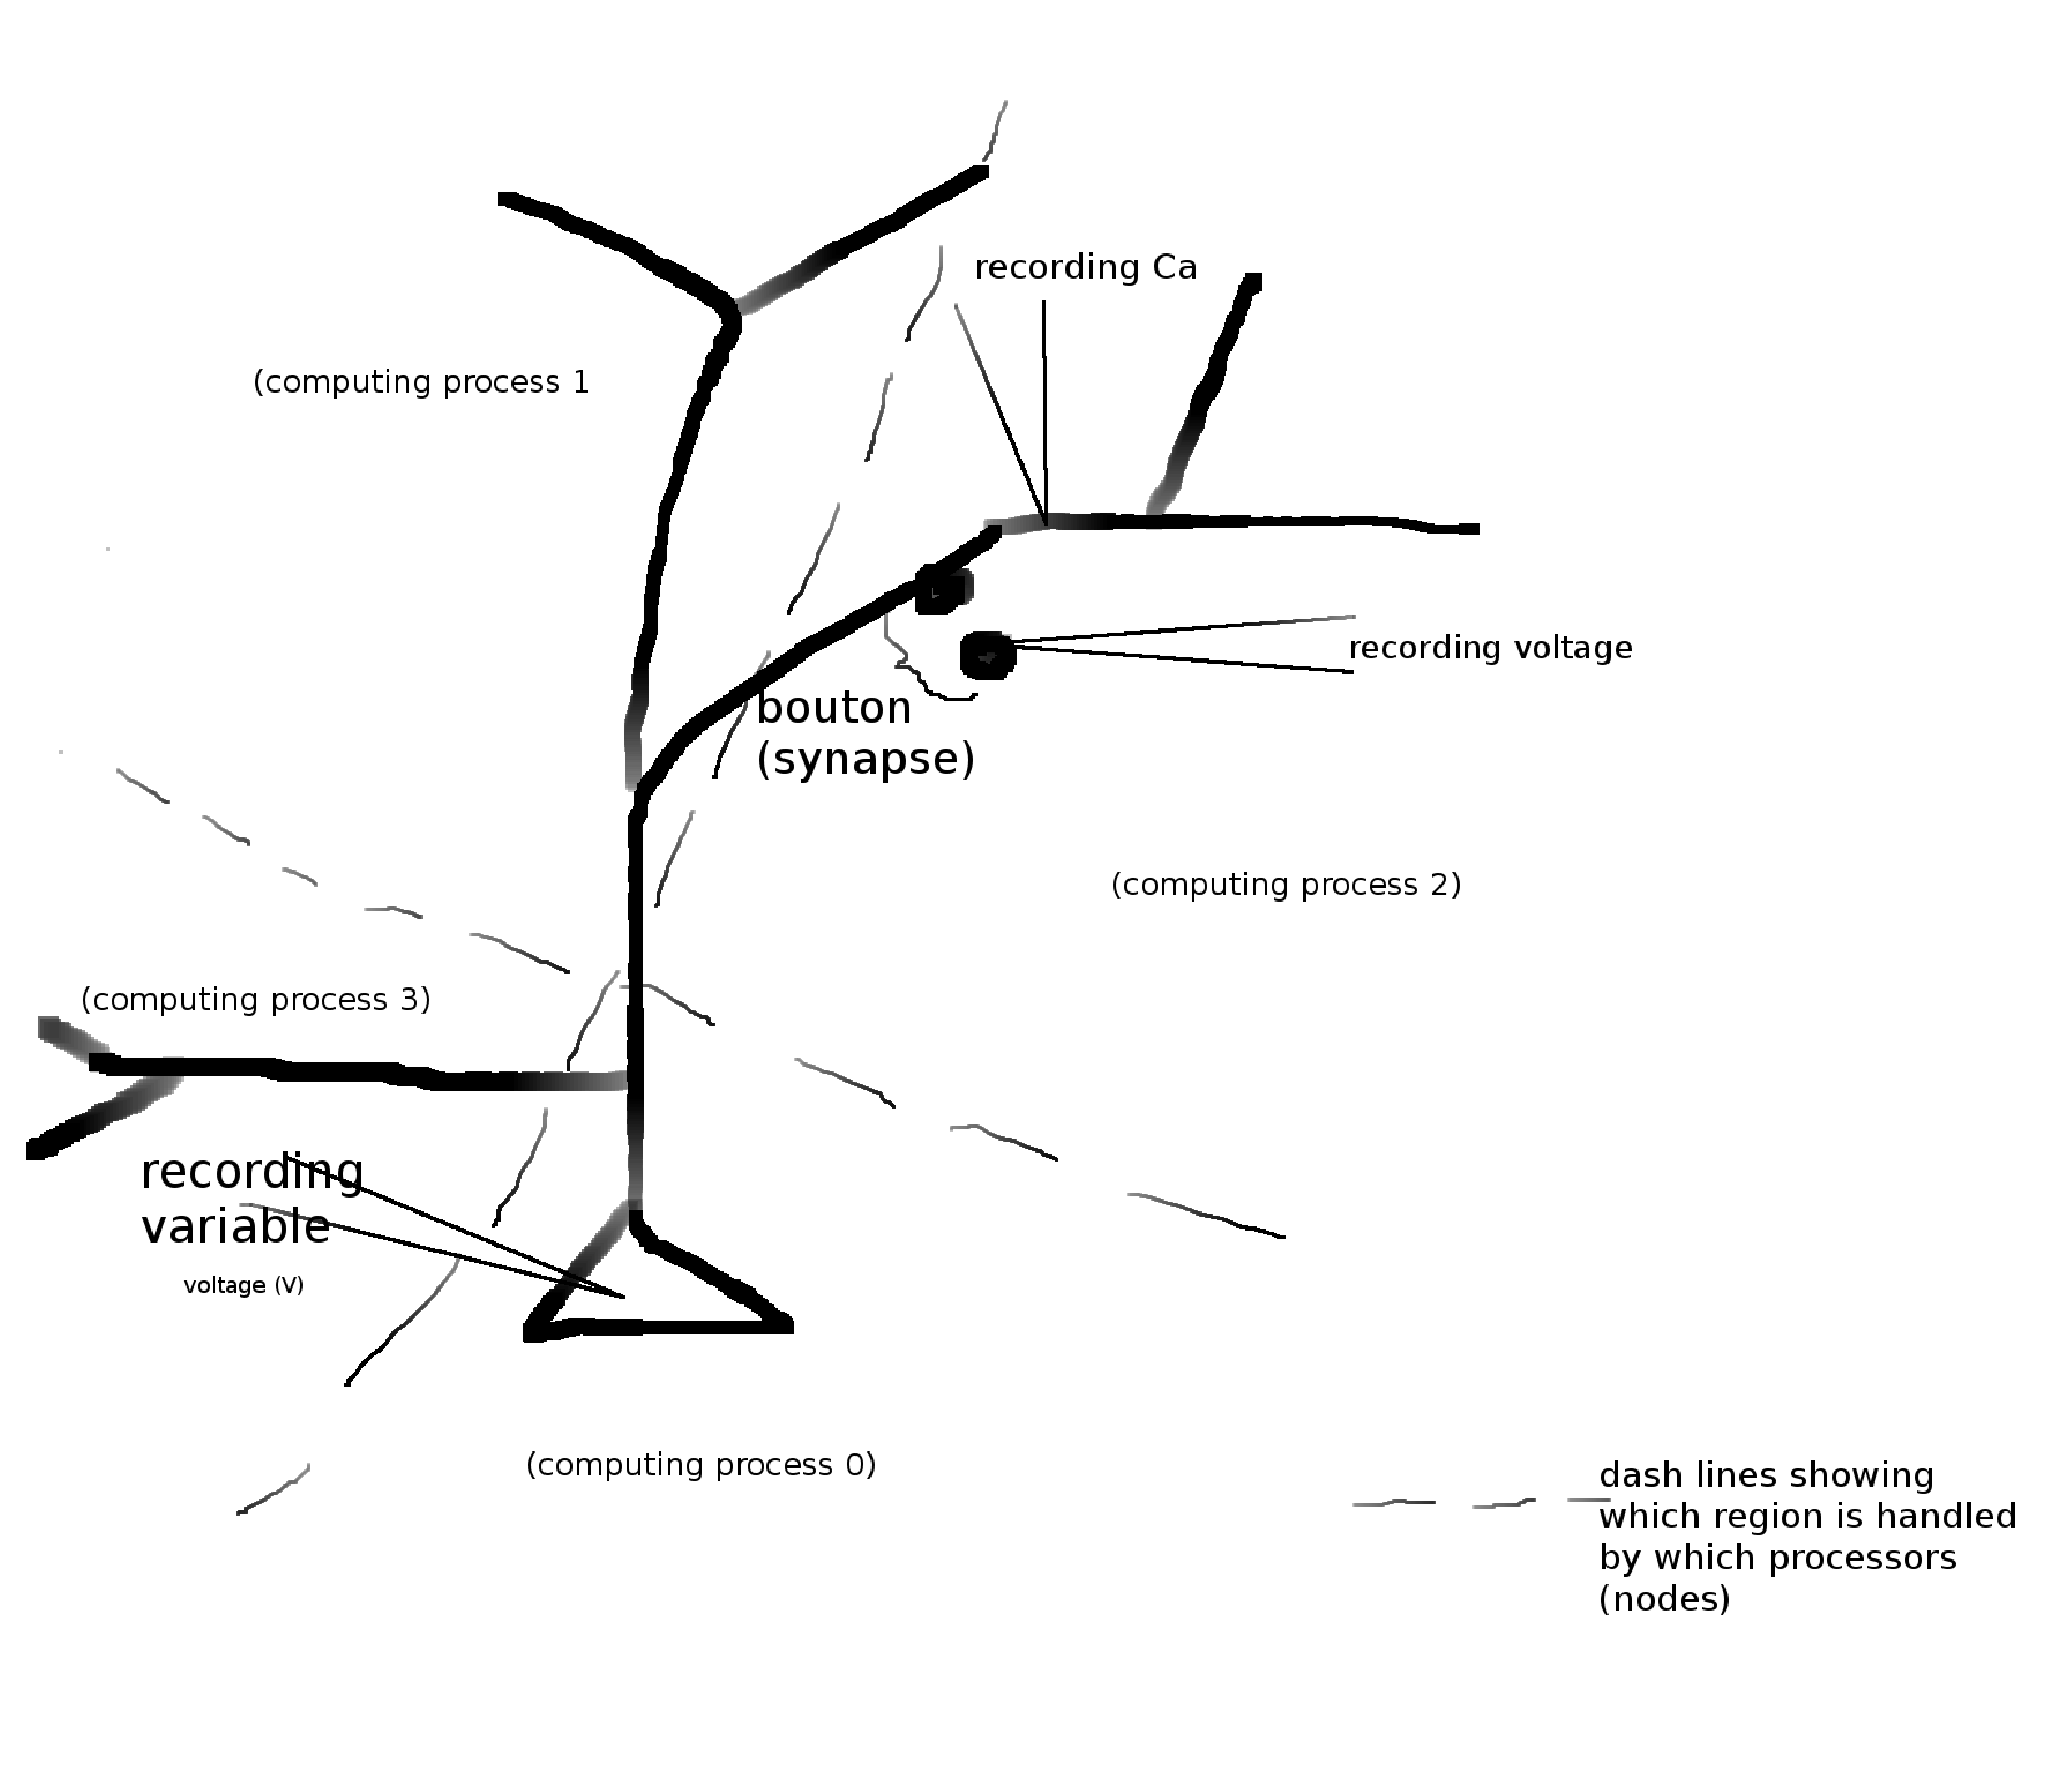
\includegraphics[height=8cm,
    angle=0]{./images/NTS_job-distribution-concept.eps}}
\caption{A schematic diagram showing how the jobs of simulating the neuron's
activity at different regions is distributed to different processes}
\label{fig:NTS_job-distribution-concept}
\end{figure}

\section{GPU port strategy}


For each Node declared in MDL (Sect.\ref{sec:MDL-component}), the data members
are defined as \verb!ShallowArray< type >! in the \verb!CG_<NodeName>! class
\begin{verbatim}
//e.g. CG_HodgkinHuxleyVoltage.h

class CG_HodgkinHuxleyVoltage
{
protected:
     ShallowArray< DimensionStruct* > dimensions;
      BranchDataStruct* branchData;
      ShallowArray< float > Aii;
      ShallowArray< float > Aip;
      ShallowArray< float > Aim;
      ShallowArray< float > RHS;
      ShallowArray< float > Aij;
      float* proximalVoltage;
      ShallowArray< float* > distalAiis;
      ShallowArray< float* > distalAips;
      ShallowArray< float* > distalInputs;
      ShallowArray< float >* valCur;
      ShallowArray< float >* valNew;
      ShallowArray< DimensionStruct* > distalDimensions;
      DimensionStruct* proximalDimension;
      bool proximalJunction;
      int computeOrder;
      ShallowArray< float > Vcur;
      ShallowArray< float > Vnew;
      float Cm;
      float cmt;
      float gLeak;
      ShallowArray< ChannelCurrents > channelCurrents;
      ShallowArray< ReceptorCurrent > receptorCurrents;
      ShallowArray< InjectedCurrent > injectedCurrents;

}

\end{verbatim}

(1) These data needs to be allocated inside GPU. The methods of ShallowArray
needs to be reimplemented to support CUDA memory allocation/resize.

\section{Macros}

\begin{verbatim}
#ifdef POLARIZED_NEURON   // Neurogenesis.cxx
#endif


\end{verbatim}

\section{Zipper}
\label{sec:NTS-Zipper}
\label{sec:Zipper-NTS}


The idea of Zipper is that
\begin{itemize}
  \item Create a special-layer: 

Example: 2 layers of 'Connexon' instances: they both have the same size; each 
\begin{verbatim}
layer-Connexon-1 --> compartment[Voltage]_neuron_1
layer-Connexon-2 --> compartment[Voltage]_neuron_2

layer-Connexon-1 <--> layer-Connexon-2

\end{verbatim}   

GOAL: We want to extract 'N' compartments from all the branches of one or
some given neuron, in this case only 1 neuron. 

CONTEXT: As the neurons can spread across MPI ranks, the number of compartments
to be extracted from that neuron on each rank is reflected through the density
vector
\begin{verbatim}
ShallowArray<int> rval;
\end{verbatim}
with the size equal to the size of the grid (X*Y*Z).

Here, the density depends on (1) the number of ComputeBranch on each
grid-point, and (2) the ComputeBranch's size, e.g.
surfaceArea.
 
In a typical layer, the number of node-instances is exactly the same as the
size of the layer, i.e. each instance occurs once.
  
This special layer is different; it can hold a vector of nodes
\begin{verbatim}
std::vector<NodeDescriptor*>
\end{verbatim}
at which a single instance can be considered multiple times.

As each instance represent the data at one compute branch, which may have
multiple compartments, the reason to have multiple occurences is that, each
occurence represent the connection to be established at a given compartment
index.

Connexon (Sect.\ref{sec:Connexon-Layer}) instances has been
allocated - just returns me a subset of such instances; and put into a new
layer.

An extension has been added to support saving the mapping order to the
associated 'Voltage' nodes as given in PRMASK0
\begin{verbatim}
#define PRMASK0 CATEGORY="BRANCH", TYPE="Voltage", BRANCHTYPE=3, MTYPE=0, NEURON_INDEX=0

Layer(DendroDendriticGapJunctionConnexons0, Connexon, tissueFunctor
    ("Layout", <PROBED="pr0", N=6, PRMASK0>), <>, tissueGM);
\end{verbatim}
What it does is
\begin{enumerate}
  \item create an implicit Layer with name 'pr0', and store all nodes matching
  the given criteria PRMASK0 into that layer.

This implicit layer is an element of this map
\begin{verbatim}
_probedNodesMap
  map< "probed-name:string, e.g. pr0",
     map< pair < "category:string, e.g. BRANCH",
                 "type:string, e.g. Voltage"
               >,
          pair<Grid*,
               std::vector<NodeDescriptor*>  // a node can be selected 
                        //more than one time
                        //as we selected compartment in that branch-node
                        //as more than one compartment can be selected
                        //in that branch 
              >
          >
       >
  >
\end{verbatim}  

This layer will be used to extract such Voltage node for establishing
connection with the Connexon later.
\begin{verbatim}
zipper(.[].Layer(DendroDendriticGapJunctionConnexons0), 
       tissueFunctor("Probe", <PROBED="pr0", PRMASK0>), outAttrDef, Mcnnxn2cpt,
       "ids0");
\end{verbatim}
Here, when it probe, it will check if the layer named 'pr0' exist, if yes
(which of course), then extract the nodes in that implicit layer. 

Here, the instance 'zipper' keeps track of the 
\end{enumerate}
  
  \item Zipper Connector: once a zipper is called, it needs to calculate the
  compartment index from each Branch/Junction to get the exact location. 
  Such locations/indices can be reused later, so they need to be stored, thus
  the last argument is the name for 'key'. Any call to the zipper, with the
  existing name, the locations/indices are reused.

A typical connector (Sect.\ref{sec:Connector}) accepts 4 parameters
\begin{verbatim}
1 = source nodeset
2 = dest   nodeset
3 = functor that operates on each node (either source-side or dest-side),
    checking it if it is a candidate for making the connection

4 = outAttrPset
5 = inAttrPset
\end{verbatim}
Example of functor in 3-rd position: EachDstFunctor (Sect.\ref{sec:EachDstFunctor})

A Zipper connector here only accepts 4 parameters; with no functor at 3-rd
position. Here, it assumes two sets have the same sizes; and performs connection
1-by-1 along the indices. 

NOTE: A \verb!NodeDescriptor*! in a Grid will be converted to a \verb!Node! in a
NodeSet.

However, as by design, only one occurrence of a given node is allowed in one
nodeset. So, the Zipper overcome this by performing a loop; each time return a
subset of non-overlap nodes. As the TissueFunctor's Probe is called to return
the vector of NodeDescriptor*, it needs a mechanism to return a subset of
non-overlapped NodeDescriptor* until it has nothing to return; and at that time;
reset the 'flag' so that next call, it will returns the whole vector again.

\end{itemize}
% //IMPORTANT: no new instances of any NodeType is created; 
% // jut new layers, each holding a subset of node instances from a given NodeType

{\tiny
\begin{verbatim}
//IMPORTANT: create new instances of a given NodeType; 
//    then manually perform all necessary connections for that NodeType

Grid Adaptor{

#define PRMASK0 CATEGORY="BRANCH", TYPE="Voltage", BRANCHTYPE=2, MTYPE=0, NEURON_INDEX=0
#define PRMASK1 CATEGORY="BRANCH", TYPE="Voltage", BRANCHTYPE=2, MTYPE=0, NEURON_INDEX=1
//{{{
   Dimension( _X_ , _Y_ , _Z_ );

//Create node instances
/* Obsolete design: no need to have ``ProbedLayout''
   Layer(DendroDendriticGapJunctionConnexons0, Connexon,
     tissueFunctor("ProbedLayout", <PROBED="pr0", N=6, PRMASK0>), <>, tissueGM); 
   Layer(DendroDendriticGapJunctionConnexons1, Connexon, tissueFunctor("ProbedLayout", <PROBED="pr1", N=6, PRMASK1>), <>, tissueGM);
*/   
   Layer(DendroDendriticGapJunctionConnexons0, Connexon, 
       tissueFunctor("Layout", <PROBED="pr0", N=6, PRMASK0>), <>, tissueGM);
   Layer(DendroDendriticGapJunctionConnexons1, Connexon, 
       tissueFunctor("Layout", <PROBED="pr1", N=6, PRMASK1>), <>, tissueGM);

//Init
   BindName cnnxn ("I", 0, "g", 0.5);
   NdplNodeInit Mcnnxn(cnnxn);

   InitNodes ( .[].Layer(DendroDendriticGapJunctionConnexons0), Mcnnxn );
   InitNodes ( .[].Layer(DendroDendriticGapJunctionConnexons1), Mcnnxn );


// Binding (connecting)
   BindName cpt2cnnxn("idx", -1,
   	 	      "identifier", "compartment[Voltage]");
   NdplInAttrInit Mcpt2cnnxn(cpt2cnnxn);

   zipper(tissueFunctor("Probe", <PROBED="pr0", PRMASK0>), .[].Layer(DendroDendriticGapJunctionConnexons0), outAttrDef, Mcpt2cnnxn, "ids0");
   zipper(tissueFunctor("Probe", <PROBED="pr1", PRMASK1>), .[].Layer(DendroDendriticGapJunctionConnexons1), outAttrDef, Mcpt2cnnxn, "ids1");

//Continue Binding
   BindName cnnxn2cpt("idx", -1,
   	 	      "identifier", "electricalSynapse[Voltage]");
   NdplInAttrInit Mcnnxn2cpt(cnnxn2cpt);
   zipper(.[].Layer(DendroDendriticGapJunctionConnexons0), tissueFunctor("Probe", <PROBED="pr0", PRMASK0>), outAttrDef, Mcnnxn2cpt, "ids0");
   zipper(.[].Layer(DendroDendriticGapJunctionConnexons1), tissueFunctor("Probe", <PROBED="pr1", PRMASK1>), outAttrDef, Mcnnxn2cpt, "ids1");
  
//}}}
}
\end{verbatim}
}

\section{Design changes}

